%%%%%%%%%%%%%%%%%%%%%%%%%%%%%%%%%%%%%%%%%
% Masters/Doctoral Thesis 
% LaTeX Template
% Version 2.5 (27/8/17)
%
% This template was downloaded from:
% http://www.LaTeXTemplates.com
%
% Version 2.x major modifications by:
% Vel (vel@latextemplates.com)
%
% This template is based on a template by:
% Steve Gunn (http://users.ecs.soton.ac.uk/srg/softwaretools/document/templates/)
% Sunil Patel (http://www.sunilpatel.co.uk/thesis-template/)
%
% Template license:
% CC BY-NC-SA 3.0 (http://creativecommons.org/licenses/by-nc-sa/3.0/)
%
%%%%%%%%%%%%%%%%%%%%%%%%%%%%%%%%%%%%%%%%%

%----------------------------------------------------------------------------------------
%	PACKAGES AND OTHER DOCUMENT CONFIGURATIONS
%----------------------------------------------------------------------------------------

\documentclass[
11pt, % The default document font size, options: 10pt, 11pt, 12pt
oneside, % Two side (alternating margins) for binding by default, uncomment to switch to one side
english, % ngerman for German
% singlespacing, % Single line spacing, alternatives: onehalfspacing or doublespacing
% TODO - something is overrulling our doublespacing, need to find out what
onehalfspacing,
%draft, % Uncomment to enable draft mode (no pictures, no links, overfull hboxes indicated)
%nolistspacing, % If the document is onehalfspacing or doublespacing, uncomment this to set spacing in lists to single
%liststotoc, % Uncomment to add the list of figures/tables/etc to the table of contents
%toctotoc, % Uncomment to add the main table of contents to the table of contents
%parskip, % Uncomment to add space between paragraphs
%nohyperref, % Uncomment to not load the hyperref package
headsepline, % Uncomment to get a line under the header
%chapterinoneline, % Uncomment to place the chapter title next to the number on one line
consistentlayout, % Uncomment to change the layout of the declaration, abstract and acknowledgements pages to match the default layout
reqno, % align equation numbers to right
]{MastersDoctoralThesis} % The class file specifying the document structure

% This goes with setspace package
% \onehalfspacing

\usepackage[utf8]{inputenc} % Required for inputting international characters
\usepackage[T1]{fontenc} % Output font encoding for international characters

\usepackage{mathpazo} % Use the Palatino font by default - Lara Chammas used this one
% Looks time TNR so let's go with that
% \usepackage{newtxmath,newtxtext} % Times New Roman - the required type
% filler to get idea of formatting
\usepackage{lipsum}
% pdf pages for appending original project proposal
\usepackage{pdfpages}

\usepackage[backend=bibtex,style=authoryear,natbib=true]{biblatex} % Use the bibtex backend with the authoryear citation style (which resembles APA)

\addbibresource{dissertation.bib} % The filename of the bibliography

\usepackage[autostyle=true]{csquotes} % Required to generate language-dependent quotes in the bibliography

\usepackage{mathtools} % for floor symbol
%----------------------------------------------------------------------------------------
%	MARGIN SETTINGS
%----------------------------------------------------------------------------------------

\geometry{
	paper=a4paper, % Change to letterpaper for US letter
	inner=2.5cm, % Inner margin
	outer=2.5cm, % Outer margin
	% bindingoffset=.5cm, % Binding offset
	top=1.5cm, % Top margin
	bottom=1.5cm, % Bottom margin
	%showframe, % Uncomment to show how the type block is set on the page
}

%----------------------------------------------------------------------------------------
%	THESIS INFORMATION
%----------------------------------------------------------------------------------------

\thesistitle{Evaluation of self-driving cars using \\ CNNs in the rain} % Your thesis title, this is used in the title and abstract, print it elsewhere with \ttitle
\supervisor{Artur Garcez} % Your supervisor's name, this is used in the title page, print it elsewhere with \supname
\examiner{} % Your examiner's name, this is not currently used anywhere in the template, print it elsewhere with \examname
\degree{Doctor of Philosophy} % Your degree name, this is used in the title page and abstract, print it elsewhere with \degreename
\author{Daniel Sikar} % Your name, this is used in the title page and abstract, print it elsewhere with \authorname
\addresses{} % Your address, this is not currently used anywhere in the template, print it elsewhere with \addressname

\subject{Biological Sciences} % Your subject area, this is not currently used anywhere in the template, print it elsewhere with \subjectname
\keywords{Autonomous Vehicles, Convolutional Neural Networks} % Keywords for your thesis, this is not currently used anywhere in the template, print it elsewhere with \keywordnames
\university{City, University of London} % Your university's name and URL, this is used in the title page and abstract, print it elsewhere with \univname
\department{\href{http://department.university.com}{Department or School Name}} % Your department's name and URL, this is used in the title page and abstract, print it elsewhere with \deptname
\group{\href{http://researchgroup.university.com}{Research Group Name}} % Your research group's name and URL, this is used in the title page, print it elsewhere with \groupname
\faculty{\href{http://faculty.university.com}{Faculty Name}} % Your faculty's name and URL, this is used in the title page and abstract, print it elsewhere with \facname

\AtBeginDocument{
\hypersetup{pdftitle=\ttitle} % Set the PDF's title to your title
\hypersetup{pdfauthor=\authorname} % Set the PDF's author to your name
\hypersetup{pdfkeywords=\keywordnames} % Set the PDF's keywords to your keywords
\hypersetup{hidelinks}
}

% do not indent paragraphs
\setlength\parindent{0pt}
% Add 
\setlength{\parskip}{0.5em} % changes vertical space between paragraphs, alternatively use pt unit e.g. {10pt} %
% Appendix
\usepackage{appendix}

\begin{document}

\frontmatter % Use roman page numbering style (i, ii, iii, iv...) for the pre-content pages

\pagestyle{plain} % Default to the plain heading style until the thesis style is called for the body content

%----------------------------------------------------------------------------------------
%	TITLE PAGE
%----------------------------------------------------------------------------------------

\begin{titlepage}
\begin{center}

\vspace*{.06\textheight}
{\scshape\LARGE \univname\par}\vspace{1.5cm} % University name
\textsc{\Large MSc in Data Science}\\[0.5cm] % Thesis type
\textsc{\Large Project Report}\\[0.5cm]
\textsc{\Large 2020}\\[0.5cm]

\HRule \\[0.4cm] % Horizontal line
{\huge \bfseries \ttitle\par}\vspace{0.4cm} % Thesis title
\HRule \\[3.5cm] % Horizontal line
 
% \begin{minipage}[t]{0.4\textwidth}
\begin{flushleft} \large
% \emph{Author:}\\
\authorname \\ [1cm]
%\href{http://www.johnsmith.com}{\authorname} % Author name - remove the \href bracket to remove the link
% \end{flushleft}
% \end{minipage}
% \begin{minipage}[t]{0.4\textwidth}
% \begin{flushright} \large

\emph{Supervised by:} 
\supname \\ [3.5cm] % Supervisor name - remove the \href bracket to remove the link  
\end{flushleft}
% \end{flushright}
%\end{minipage}\\[3cm]
 

%\large \textit{A thesis submitted in fulfillment of the requirements\\ for the degree of %\degreename}\\[0.3cm] % University requirement text
%\textit{in the}\\[0.4cm]
%\groupname\\\deptname\\[2cm] % Research group name and department name
 

{\large \today}\\[4cm] % Date
%\includegraphics{Logo} % University/department logo - uncomment to place it
 
%vfill
\end{center}
\end{titlepage}

%----------------------------------------------------------------------------------------
%	DECLARATION PAGE
%----------------------------------------------------------------------------------------

\begin{declaration}
\addchaptertocentry{\authorshipname} % Add the declaration to the table of contents
\noindent By submitting this work, I declare that this work is entirely my own except those parts duly identified and referenced in my submission. It complies with any specified word limits and the requirements and regulations detailed in the assessment instructions and any other relevant programme and module documentation. In submitting this work I acknowledge that I have read and understood the regulations and code regarding academic misconduct, including that relating to plagiarism, as specified in the Programme Handbook. I also acknowledge that this work will be subject to a variety of checks for academic misconduct. \\[1cm]
 
\noindent Signed:\\[1cm]
\authorname 
%Daniel Sikar
%\rule[0.5em]{25em}{0.5pt} % This prints a line for the signature
 
%\noindent Date:\\
%\rule[0.5em]{25em}{0.5pt} % This prints a line to write the date
\end{declaration}

\cleardoublepage

% \begin{declaration}
% \addchaptertocentry{\authorshipname} % Add the declaration to the table of contents
%\noindent By submitting this work, I declare that this work is entirely my own except those parts duly identified and referenced in my submission. It complies with any specified word limits and the requirements and regulations detailed in the assessment instructions and any other relevant programme and module documentation. In submitting this work I acknowledge that I have read and understood the regulations and code regarding academic misconduct, including that relating to plagiarism, as specified in the Programme Handbook. I also acknowledge that this work will be subject to a variety of checks for academic misconduct. \\[1cm]
 
%\noindent Signed:\\[1cm]
%Daniel Sikar
%\rule[0.5em]{25em}{0.5pt} % This prints a line for the signature
 
%\noindent Date:\\
%\rule[0.5em]{25em}{0.5pt} % This prints a line to write the date
%\end{declaration}

\cleardoublepage

%----------------------------------------------------------------------------------------
%	QUOTATION PAGE
%----------------------------------------------------------------------------------------

%\vspace*{0.2\textheight}

%\noindent\enquote{\itshape Thanks to my solid academic training, today I can write hundreds of words on virtually any topic without possessing a shred of information, which is how I got a good job in journalism.}\bigbreak

%\hfill Dave Barry

%----------------------------------------------------------------------------------------
%	ABSTRACT PAGE
%----------------------------------------------------------------------------------------

%----------------------------------------------------------------------------------------
%	ABSTRACT PAGE
%----------------------------------------------------------------------------------------

\begin{abstract}
% LC - 181 words - https://wordcounter.net/
\addchaptertocentry{\abstractname} % Add the abstract to the table of contents

%%% APPLICATION AND SUCCESS STORY OF CONVNETS 
%%% ConvNets has found success in diverse areas.
%%% Deep learning has found successful application in diverse areas
%%% including end-to-end self-driving cars, where a trained model is given an image and outputs values such as steering and throttle.

%%% THE PROBLEM WE ARE DEALING WITH - cONVNETS LACKING ROBUSTNESS E.G. ONE-PIXEL-ATTACKS, RANDOM LABELS (BENGIO ET AL)
% However, there is a problem - noisy images

%%% WHAT WE DID - maybe leave the nitty gritty for later e.g. Unity 3D ?
This project investigates the effect of rainy images on the performance of end to end convolutional neural networks (CNNs) applied to self-driving cars, using public domain real-world datasets, as well as data synthetically generated by the Unity 3D gaming engine. 
%%% WHAT WE FOUND

% we need an angle here on the bigger picture of end-to-end learning of which self-driving cars training with behavioural learning are a specific case.
% Like a survey on end-to-end applications

% TODO end-to-end applications, one or two paragraphs, maybe in the intro or context.


%%% Results suggest that random noise does have a detrimental effect on network performance which may be mitigated by 

CNNs have become state-of-the-art in supervised image classification tasks, used in both \textit{pipelined} and \textit{end-to-end} architectures. the former relying on a fusion of image and sensor data the latter on images alone, to determine steering and movement output.  
However, CNNs applied to image classification have been shown to lack robustness when, given noisy images, in some cases a single pixel change, are known to output incorrect results that for humans would have been obviously the same as the denoised versions.
As deep learning models, be it CNNs, Recurrent Neural Networks or Deep Reinforcement Learning Networks rely increasingly on computer vision for robotics in general, and for self-driving cars in particular, it is important to evaluate the effect of noise, such as images containing rain, used by such models.
This study provides a novel testing environment that is able to subject self-driving CNN architectures to different rain levels, which may inform design decisions relating to safety.
% WHAT WE FOUND
% Results suggest that image pre-processing may be used to neutralise the effect of noise such as rainy images.

% This study is to the best of my knowledge the first of its kind.

%%% By training and testing resulting models with the Unity 3D game engine, we provide
  
\vspace{25mm} %5mm vertical space
  
  
\textbf{Keywords:} autonomous vehicles, convolutional neural networks, rain noise

\end{abstract}

%----------------------
%	ACKNOWLEDGEMENTS
%----------------------

%\begin{acknowledgements}
%\addchaptertocentry{\acknowledgementname} % Add the acknowledgements to the table of contents
%The acknowledgments and the people to thank go here, don't forget to include your project %advisor\ldots
%\end{acknowledgements}

%----------------------------------------------------------------------------------------
%	LIST OF CONTENTS/FIGURES/TABLES PAGES
%----------------------------------------------------------------------------------------

\tableofcontents % Prints the main table of contents

% \listoffigures % Prints the list of figures

% \listoftables % Prints the list of tables

%----------------------------------------------------------------------------------------
%	ABBREVIATIONS
%----------------------------------------------------------------------------------------

%\begin{abbreviations}{ll} % Include a list of abbreviations (a table of two columns)

%\textbf{LAH} & \textbf{L}ist \textbf{A}bbreviations \textbf{H}ere\\
%\textbf{WSF} & \textbf{W}hat (it) \textbf{S}tands \textbf{F}or\\

%\end{abbreviations}

%----------------------------------------------------------------------------------------
%	PHYSICAL CONSTANTS/OTHER DEFINITIONS
%----------------------------------------------------------------------------------------

%\begin{constants}{lr@{${}={}$}l} % The list of physical constants is a three column table

% The \SI{}{} command is provided by the siunitx package, see its documentation for instructions on how to use it

%Speed of Light & $c_{0}$ & \SI{2.99792458e8}{\meter\per\second} (exact)\\
%Constant Name & $Symbol$ & $Constant Value$ with units\\

%\end{constants}

%----------------------------------------------------------------------------------------
%	SYMBOLS
%----------------------------------------------------------------------------------------

%\begin{symbols}{lll} % Include a list of Symbols (a three column table)

%$a$ & distance & \si{\meter} \\
%$P$ & power & \si{\watt} (\si{\joule\per\second}) \\
%Symbol & Name & Unit \\

%\addlinespace % Gap to separate the Roman symbols from the Greek

%$\omega$ & angular frequency & \si{\radian} \\

%\end{symbols}

%----------------------------------------------------------------------------------------
%	DEDICATION
%----------------------------------------------------------------------------------------

% \dedicatory{For/Dedicated to/To my\ldots} 

%----------------------------------------------------------------------------------------
%	THESIS CONTENT - CHAPTERS
%----------------------------------------------------------------------------------------

\mainmatter % Begin numeric (1,2,3...) page numbering

\pagestyle{thesis} % Return the page headers back to the "thesis" style

% Include the chapters of the thesis as separate files from the Chapters folder
% Uncomment the lines as you write the chapters

%% Chapter 1

\chapter{Chapter Title Here} % Main chapter title

\label{Chapter1} % For referencing the chapter elsewhere, use \ref{Chapter1} 

%----------------------------------------------------------------------------------------

% Define some commands to keep the formatting separated from the content 
\newcommand{\keyword}[1]{\textbf{#1}}
\newcommand{\tabhead}[1]{\textbf{#1}}
\newcommand{\code}[1]{\texttt{#1}}
\newcommand{\file}[1]{\texttt{\bfseries#1}}
\newcommand{\option}[1]{\texttt{\itshape#1}}

%----------------------------------------------------------------------------------------

\section{Welcome and Thank You}
Welcome to this \LaTeX{} Thesis Template, a beautiful and easy to use template for writing a thesis using the \LaTeX{} typesetting system.

If you are writing a thesis (or will be in the future) and its subject is technical or mathematical (though it doesn't have to be), then creating it in \LaTeX{} is highly recommended as a way to make sure you can just get down to the essential writing without having to worry over formatting or wasting time arguing with your word processor.

\LaTeX{} is easily able to professionally typeset documents that run to hundreds or thousands of pages long. With simple mark-up commands, it automatically sets out the table of contents, margins, page headers and footers and keeps the formatting consistent and beautiful. One of its main strengths is the way it can easily typeset mathematics, even \emph{heavy} mathematics. Even if those equations are the most horribly twisted and most difficult mathematical problems that can only be solved on a super-computer, you can at least count on \LaTeX{} to make them look stunning.

%----------------------------------------------------------------------------------------

\section{Learning \LaTeX{}}

\LaTeX{} is not a \textsc{wysiwyg} (What You See is What You Get) program, unlike word processors such as Microsoft Word or Apple's Pages. Instead, a document written for \LaTeX{} is actually a simple, plain text file that contains \emph{no formatting}. You tell \LaTeX{} how you want the formatting in the finished document by writing in simple commands amongst the text, for example, if I want to use \emph{italic text for emphasis}, I write the \verb|\emph{text}| command and put the text I want in italics in between the curly braces. This means that \LaTeX{} is a \enquote{mark-up} language, very much like HTML.

\subsection{A (not so short) Introduction to \LaTeX{}}

If you are new to \LaTeX{}, there is a very good eBook -- freely available online as a PDF file -- called, \enquote{The Not So Short Introduction to \LaTeX{}}. The book's title is typically shortened to just \emph{lshort}. You can download the latest version (as it is occasionally updated) from here:
\url{http://www.ctan.org/tex-archive/info/lshort/english/lshort.pdf}

It is also available in several other languages. Find yours from the list on this page: \url{http://www.ctan.org/tex-archive/info/lshort/}

It is recommended to take a little time out to learn how to use \LaTeX{} by creating several, small `test' documents, or having a close look at several templates on:\\ 
\url{http://www.LaTeXTemplates.com}\\ 
Making the effort now means you're not stuck learning the system when what you \emph{really} need to be doing is writing your thesis.

\subsection{A Short Math Guide for \LaTeX{}}

If you are writing a technical or mathematical thesis, then you may want to read the document by the AMS (American Mathematical Society) called, \enquote{A Short Math Guide for \LaTeX{}}. It can be found online here:
\url{http://www.ams.org/tex/amslatex.html}
under the \enquote{Additional Documentation} section towards the bottom of the page.

\subsection{Common \LaTeX{} Math Symbols}
There are a multitude of mathematical symbols available for \LaTeX{} and it would take a great effort to learn the commands for them all. The most common ones you are likely to use are shown on this page:
\url{http://www.sunilpatel.co.uk/latex-type/latex-math-symbols/}

You can use this page as a reference or crib sheet, the symbols are rendered as large, high quality images so you can quickly find the \LaTeX{} command for the symbol you need.

\subsection{\LaTeX{} on a Mac}
 
The \LaTeX{} distribution is available for many systems including Windows, Linux and Mac OS X. The package for OS X is called MacTeX and it contains all the applications you need -- bundled together and pre-customized -- for a fully working \LaTeX{} environment and work flow.
 
MacTeX includes a custom dedicated \LaTeX{} editor called TeXShop for writing your `\file{.tex}' files and BibDesk: a program to manage your references and create your bibliography section just as easily as managing songs and creating playlists in iTunes.

%----------------------------------------------------------------------------------------

\section{Getting Started with this Template}

If you are familiar with \LaTeX{}, then you should explore the directory structure of the template and then proceed to place your own information into the \emph{THESIS INFORMATION} block of the \file{main.tex} file. You can then modify the rest of this file to your unique specifications based on your degree/university. Section \ref{FillingFile} on page \pageref{FillingFile} will help you do this. Make sure you also read section \ref{ThesisConventions} about thesis conventions to get the most out of this template.

If you are new to \LaTeX{} it is recommended that you carry on reading through the rest of the information in this document.

Before you begin using this template you should ensure that its style complies with the thesis style guidelines imposed by your institution. In most cases this template style and layout will be suitable. If it is not, it may only require a small change to bring the template in line with your institution's recommendations. These modifications will need to be done on the \file{MastersDoctoralThesis.cls} file.

\subsection{About this Template}

This \LaTeX{} Thesis Template is originally based and created around a \LaTeX{} style file created by Steve R.\ Gunn from the University of Southampton (UK), department of Electronics and Computer Science. You can find his original thesis style file at his site, here:
\url{http://www.ecs.soton.ac.uk/~srg/softwaretools/document/templates/}

Steve's \file{ecsthesis.cls} was then taken by Sunil Patel who modified it by creating a skeleton framework and folder structure to place the thesis files in. The resulting template can be found on Sunil's site here:
\url{http://www.sunilpatel.co.uk/thesis-template}

Sunil's template was made available through \url{http://www.LaTeXTemplates.com} where it was modified many times based on user requests and questions. Version 2.0 and onwards of this template represents a major modification to Sunil's template and is, in fact, hardly recognisable. The work to make version 2.0 possible was carried out by \href{mailto:vel@latextemplates.com}{Vel} and Johannes Böttcher.

%----------------------------------------------------------------------------------------

\section{What this Template Includes}

\subsection{Folders}

This template comes as a single zip file that expands out to several files and folders. The folder names are mostly self-explanatory:

\keyword{Appendices} -- this is the folder where you put the appendices. Each appendix should go into its own separate \file{.tex} file. An example and template are included in the directory.

\keyword{Chapters} -- this is the folder where you put the thesis chapters. A thesis usually has about six chapters, though there is no hard rule on this. Each chapter should go in its own separate \file{.tex} file and they can be split as:
\begin{itemize}
\item Chapter 1: Introduction to the thesis topic
\item Chapter 2: Background information and theory
\item Chapter 3: (Laboratory) experimental setup
\item Chapter 4: Details of experiment 1
\item Chapter 5: Details of experiment 2
\item Chapter 6: Discussion of the experimental results
\item Chapter 7: Conclusion and future directions
\end{itemize}
This chapter layout is specialised for the experimental sciences, your discipline may be different.

\keyword{Figures} -- this folder contains all figures for the thesis. These are the final images that will go into the thesis document.

\subsection{Files}

Included are also several files, most of them are plain text and you can see their contents in a text editor. After initial compilation, you will see that more auxiliary files are created by \LaTeX{} or BibTeX and which you don't need to delete or worry about:

\keyword{example.bib} -- this is an important file that contains all the bibliographic information and references that you will be citing in the thesis for use with BibTeX. You can write it manually, but there are reference manager programs available that will create and manage it for you. Bibliographies in \LaTeX{} are a large subject and you may need to read about BibTeX before starting with this. Many modern reference managers will allow you to export your references in BibTeX format which greatly eases the amount of work you have to do.

\keyword{MastersDoctoralThesis.cls} -- this is an important file. It is the class file that tells \LaTeX{} how to format the thesis. 

\keyword{main.pdf} -- this is your beautifully typeset thesis (in the PDF file format) created by \LaTeX{}. It is supplied in the PDF with the template and after you compile the template you should get an identical version.

\keyword{main.tex} -- this is an important file. This is the file that you tell \LaTeX{} to compile to produce your thesis as a PDF file. It contains the framework and constructs that tell \LaTeX{} how to layout the thesis. It is heavily commented so you can read exactly what each line of code does and why it is there. After you put your own information into the \emph{THESIS INFORMATION} block -- you have now started your thesis!

Files that are \emph{not} included, but are created by \LaTeX{} as auxiliary files include:

\keyword{main.aux} -- this is an auxiliary file generated by \LaTeX{}, if it is deleted \LaTeX{} simply regenerates it when you run the main \file{.tex} file.

\keyword{main.bbl} -- this is an auxiliary file generated by BibTeX, if it is deleted, BibTeX simply regenerates it when you run the \file{main.aux} file. Whereas the \file{.bib} file contains all the references you have, this \file{.bbl} file contains the references you have actually cited in the thesis and is used to build the bibliography section of the thesis.

\keyword{main.blg} -- this is an auxiliary file generated by BibTeX, if it is deleted BibTeX simply regenerates it when you run the main \file{.aux} file.

\keyword{main.lof} -- this is an auxiliary file generated by \LaTeX{}, if it is deleted \LaTeX{} simply regenerates it when you run the main \file{.tex} file. It tells \LaTeX{} how to build the \emph{List of Figures} section.

\keyword{main.log} -- this is an auxiliary file generated by \LaTeX{}, if it is deleted \LaTeX{} simply regenerates it when you run the main \file{.tex} file. It contains messages from \LaTeX{}, if you receive errors and warnings from \LaTeX{}, they will be in this \file{.log} file.

\keyword{main.lot} -- this is an auxiliary file generated by \LaTeX{}, if it is deleted \LaTeX{} simply regenerates it when you run the main \file{.tex} file. It tells \LaTeX{} how to build the \emph{List of Tables} section.

\keyword{main.out} -- this is an auxiliary file generated by \LaTeX{}, if it is deleted \LaTeX{} simply regenerates it when you run the main \file{.tex} file.

So from this long list, only the files with the \file{.bib}, \file{.cls} and \file{.tex} extensions are the most important ones. The other auxiliary files can be ignored or deleted as \LaTeX{} and BibTeX will regenerate them.

%----------------------------------------------------------------------------------------

\section{Filling in Your Information in the \file{main.tex} File}\label{FillingFile}

You will need to personalise the thesis template and make it your own by filling in your own information. This is done by editing the \file{main.tex} file in a text editor or your favourite LaTeX environment.

Open the file and scroll down to the third large block titled \emph{THESIS INFORMATION} where you can see the entries for \emph{University Name}, \emph{Department Name}, etc \ldots

Fill out the information about yourself, your group and institution. You can also insert web links, if you do, make sure you use the full URL, including the \code{http://} for this. If you don't want these to be linked, simply remove the \verb|\href{url}{name}| and only leave the name.

When you have done this, save the file and recompile \code{main.tex}. All the information you filled in should now be in the PDF, complete with web links. You can now begin your thesis proper!

%----------------------------------------------------------------------------------------

\section{The \code{main.tex} File Explained}

The \file{main.tex} file contains the structure of the thesis. There are plenty of written comments that explain what pages, sections and formatting the \LaTeX{} code is creating. Each major document element is divided into commented blocks with titles in all capitals to make it obvious what the following bit of code is doing. Initially there seems to be a lot of \LaTeX{} code, but this is all formatting, and it has all been taken care of so you don't have to do it.

Begin by checking that your information on the title page is correct. For the thesis declaration, your institution may insist on something different than the text given. If this is the case, just replace what you see with what is required in the \emph{DECLARATION PAGE} block.

Then comes a page which contains a funny quote. You can put your own, or quote your favourite scientist, author, person, and so on. Make sure to put the name of the person who you took the quote from.

Following this is the abstract page which summarises your work in a condensed way and can almost be used as a standalone document to describe what you have done. The text you write will cause the heading to move up so don't worry about running out of space.

Next come the acknowledgements. On this page, write about all the people who you wish to thank (not forgetting parents, partners and your advisor/supervisor).

The contents pages, list of figures and tables are all taken care of for you and do not need to be manually created or edited. The next set of pages are more likely to be optional and can be deleted since they are for a more technical thesis: insert a list of abbreviations you have used in the thesis, then a list of the physical constants and numbers you refer to and finally, a list of mathematical symbols used in any formulae. Making the effort to fill these tables means the reader has a one-stop place to refer to instead of searching the internet and references to try and find out what you meant by certain abbreviations or symbols.

The list of symbols is split into the Roman and Greek alphabets. Whereas the abbreviations and symbols ought to be listed in alphabetical order (and this is \emph{not} done automatically for you) the list of physical constants should be grouped into similar themes.

The next page contains a one line dedication. Who will you dedicate your thesis to?

Finally, there is the block where the chapters are included. Uncomment the lines (delete the \code{\%} character) as you write the chapters. Each chapter should be written in its own file and put into the \emph{Chapters} folder and named \file{Chapter1}, \file{Chapter2}, etc\ldots Similarly for the appendices, uncomment the lines as you need them. Each appendix should go into its own file and placed in the \emph{Appendices} folder.

After the preamble, chapters and appendices finally comes the bibliography. The bibliography style (called \option{authoryear}) is used for the bibliography and is a fully featured style that will even include links to where the referenced paper can be found online. Do not underestimate how grateful your reader will be to find that a reference to a paper is just a click away. Of course, this relies on you putting the URL information into the BibTeX file in the first place.

%----------------------------------------------------------------------------------------

\section{Thesis Features and Conventions}\label{ThesisConventions}

To get the best out of this template, there are a few conventions that you may want to follow.

One of the most important (and most difficult) things to keep track of in such a long document as a thesis is consistency. Using certain conventions and ways of doing things (such as using a Todo list) makes the job easier. Of course, all of these are optional and you can adopt your own method.

\subsection{Printing Format}

This thesis template is designed for double sided printing (i.e. content on the front and back of pages) as most theses are printed and bound this way. Switching to one sided printing is as simple as uncommenting the \option{oneside} option of the \code{documentclass} command at the top of the \file{main.tex} file. You may then wish to adjust the margins to suit specifications from your institution.

The headers for the pages contain the page number on the outer side (so it is easy to flick through to the page you want) and the chapter name on the inner side.

The text is set to 11 point by default with single line spacing, again, you can tune the text size and spacing should you want or need to using the options at the very start of \file{main.tex}. The spacing can be changed similarly by replacing the \option{singlespacing} with \option{onehalfspacing} or \option{doublespacing}.

\subsection{Using US Letter Paper}

The paper size used in the template is A4, which is the standard size in Europe. If you are using this thesis template elsewhere and particularly in the United States, then you may have to change the A4 paper size to the US Letter size. This can be done in the margins settings section in \file{main.tex}.

Due to the differences in the paper size, the resulting margins may be different to what you like or require (as it is common for institutions to dictate certain margin sizes). If this is the case, then the margin sizes can be tweaked by modifying the values in the same block as where you set the paper size. Now your document should be set up for US Letter paper size with suitable margins.

\subsection{References}

The \code{biblatex} package is used to format the bibliography and inserts references such as this one \parencite{Reference1}. The options used in the \file{main.tex} file mean that the in-text citations of references are formatted with the author(s) listed with the date of the publication. Multiple references are separated by semicolons (e.g. \parencite{Reference2, Reference1}) and references with more than three authors only show the first author with \emph{et al.} indicating there are more authors (e.g. \parencite{Reference3}). This is done automatically for you. To see how you use references, have a look at the \file{Chapter1.tex} source file. Many reference managers allow you to simply drag the reference into the document as you type.

Scientific references should come \emph{before} the punctuation mark if there is one (such as a comma or period). The same goes for footnotes\footnote{Such as this footnote, here down at the bottom of the page.}. You can change this but the most important thing is to keep the convention consistent throughout the thesis. Footnotes themselves should be full, descriptive sentences (beginning with a capital letter and ending with a full stop). The APA6 states: \enquote{Footnote numbers should be superscripted, [...], following any punctuation mark except a dash.} The Chicago manual of style states: \enquote{A note number should be placed at the end of a sentence or clause. The number follows any punctuation mark except the dash, which it precedes. It follows a closing parenthesis.}

The bibliography is typeset with references listed in alphabetical order by the first author's last name. This is similar to the APA referencing style. To see how \LaTeX{} typesets the bibliography, have a look at the very end of this document (or just click on the reference number links in in-text citations).

\subsubsection{A Note on bibtex}

The bibtex backend used in the template by default does not correctly handle unicode character encoding (i.e. "international" characters). You may see a warning about this in the compilation log and, if your references contain unicode characters, they may not show up correctly or at all. The solution to this is to use the biber backend instead of the outdated bibtex backend. This is done by finding this in \file{main.tex}: \option{backend=bibtex} and changing it to \option{backend=biber}. You will then need to delete all auxiliary BibTeX files and navigate to the template directory in your terminal (command prompt). Once there, simply type \code{biber main} and biber will compile your bibliography. You can then compile \file{main.tex} as normal and your bibliography will be updated. An alternative is to set up your LaTeX editor to compile with biber instead of bibtex, see \href{http://tex.stackexchange.com/questions/154751/biblatex-with-biber-configuring-my-editor-to-avoid-undefined-citations/}{here} for how to do this for various editors.

\subsection{Tables}

Tables are an important way of displaying your results, below is an example table which was generated with this code:

{\small
\begin{verbatim}
\begin{table}
\caption{The effects of treatments X and Y on the four groups studied.}
\label{tab:treatments}
\centering
\begin{tabular}{l l l}
\toprule
\tabhead{Groups} & \tabhead{Treatment X} & \tabhead{Treatment Y} \\
\midrule
1 & 0.2 & 0.8\\
2 & 0.17 & 0.7\\
3 & 0.24 & 0.75\\
4 & 0.68 & 0.3\\
\bottomrule\\
\end{tabular}
\end{table}
\end{verbatim}
}

\begin{table}
\caption{The effects of treatments X and Y on the four groups studied.}
\label{tab:treatments}
\centering
\begin{tabular}{l l l}
\toprule
\tabhead{Groups} & \tabhead{Treatment X} & \tabhead{Treatment Y} \\
\midrule
1 & 0.2 & 0.8\\
2 & 0.17 & 0.7\\
3 & 0.24 & 0.75\\
4 & 0.68 & 0.3\\
\bottomrule\\
\end{tabular}
\end{table}

You can reference tables with \verb|\ref{<label>}| where the label is defined within the table environment. See \file{Chapter1.tex} for an example of the label and citation (e.g. Table~\ref{tab:treatments}).

\subsection{Figures}

There will hopefully be many figures in your thesis (that should be placed in the \emph{Figures} folder). The way to insert figures into your thesis is to use a code template like this:
\begin{verbatim}
\begin{figure}
\centering

\includegraphics{Figures/Electron}
\decoRule
\caption[An Electron]{An electron (artist's impression).}
\label{fig:Electron}
\end{figure}
\end{verbatim}
Also look in the source file. Putting this code into the source file produces the picture of the electron that you can see in the figure below.

\begin{figure}[th]
\centering

\includegraphics{Figures/Electron}
\decoRule
\caption[An Electron]{An electron (artist's impression).}
\label{fig:Electron}
\end{figure}

Sometimes figures don't always appear where you write them in the source. The placement depends on how much space there is on the page for the figure. Sometimes there is not enough room to fit a figure directly where it should go (in relation to the text) and so \LaTeX{} puts it at the top of the next page. Positioning figures is the job of \LaTeX{} and so you should only worry about making them look good!

Figures usually should have captions just in case you need to refer to them (such as in Figure~\ref{fig:Electron}). The \verb|\caption| command contains two parts, the first part, inside the square brackets is the title that will appear in the \emph{List of Figures}, and so should be short. The second part in the curly brackets should contain the longer and more descriptive caption text.

The \verb|\decoRule| command is optional and simply puts an aesthetic horizontal line below the image. If you do this for one image, do it for all of them.

\LaTeX{} is capable of using images in pdf, jpg and png format.

\subsection{Typesetting mathematics}

If your thesis is going to contain heavy mathematical content, be sure that \LaTeX{} will make it look beautiful, even though it won't be able to solve the equations for you.

The \enquote{Not So Short Introduction to \LaTeX} (available on \href{http://www.ctan.org/tex-archive/info/lshort/english/lshort.pdf}{CTAN}) should tell you everything you need to know for most cases of typesetting mathematics. If you need more information, a much more thorough mathematical guide is available from the AMS called, \enquote{A Short Math Guide to \LaTeX} and can be downloaded from:
\url{ftp://ftp.ams.org/pub/tex/doc/amsmath/short-math-guide.pdf}

There are many different \LaTeX{} symbols to remember, luckily you can find the most common symbols in \href{http://ctan.org/pkg/comprehensive}{The Comprehensive \LaTeX~Symbol List}.

You can write an equation, which is automatically given an equation number by \LaTeX{} like this:
\begin{verbatim}
\begin{equation}
E = mc^{2}
\label{eqn:Einstein}
\end{equation}
\end{verbatim}

This will produce Einstein's famous energy-matter equivalence equation:
\begin{equation}
E = mc^{2}
\label{eqn:Einstein}
\end{equation}

All equations you write (which are not in the middle of paragraph text) are automatically given equation numbers by \LaTeX{}. If you don't want a particular equation numbered, use the unnumbered form:
\begin{verbatim}
\[ a^{2}=4 \]
\end{verbatim}

%----------------------------------------------------------------------------------------

\section{Sectioning and Subsectioning}

You should break your thesis up into nice, bite-sized sections and subsections. \LaTeX{} automatically builds a table of Contents by looking at all the \verb|\chapter{}|, \verb|\section{}|  and \verb|\subsection{}| commands you write in the source.

The Table of Contents should only list the sections to three (3) levels. A \verb|chapter{}| is level zero (0). A \verb|\section{}| is level one (1) and so a \verb|\subsection{}| is level two (2). In your thesis it is likely that you will even use a \verb|subsubsection{}|, which is level three (3). The depth to which the Table of Contents is formatted is set within \file{MastersDoctoralThesis.cls}. If you need this changed, you can do it in \file{main.tex}.

%----------------------------------------------------------------------------------------

\section{In Closing}

You have reached the end of this mini-guide. You can now rename or overwrite this pdf file and begin writing your own \file{Chapter1.tex} and the rest of your thesis. The easy work of setting up the structure and framework has been taken care of for you. It's now your job to fill it out!

Good luck and have lots of fun!

\begin{flushright}
Guide written by ---\\
Sunil Patel: \href{http://www.sunilpatel.co.uk}{www.sunilpatel.co.uk}\\
Vel: \href{http://www.LaTeXTemplates.com}{LaTeXTemplates.com}
\end{flushright}

% TODO COMMENT ALL IN FOR FINAL COMPILE
%
\chapter{Introduction and Objectives}

\label{Intro} 

%%% Introduction and Objectives: This chapter should set the scene for the reader. It must outline the background to the problem, give your reasons for the choice of project, and identify the project’s beneficiaries. Your objectives need to be precisely stated, together with the tests that will show, at the end of the project, that they have been met (or not been met). You need also to outline your methods in broad terms, along with y work plan with sufficient detail to show how you planned to meet the objectives. Outline any major changes of goals or methods that happened during the project. Finally, outline the structure of the report, showing how it fits together.

%-----------------------------------
%	BACKGROUND
%-----------------------------------

\section{Background}

% Chammas - 503 words, 7 references
% references
% 1. Self driving robot with Mainframe processor
% 2. European investment, Dickmans
% 3. Carnegie Melon
% 4. Darpa
% 5. Dave
% 6. NVIDIA

% Paragraph 1
% The goal of self driving cars...
% Self-driving cars are a difficult problem to solve...

% Paragraph 2
% With advances in deep learning, training algorithms and computational power...
%% Research question
%% Given the above, how reliable are self-driving cars relying on end-to-end ConvNets in the rain?
%% This project builds on something or other, uses natural and synthetic datasets

% What motivates the study of autonomous vehicles
The development of self-driving cars, a particular case of autonomous vehicle (AV), is motivated by a number of goals, of a practical, safety, public interest and economic nature.
%% Practical goal
 From a practical perspective, the goal is "to transport people from one place to another without any help from a driver" (\cite{s20092544}).
 %% Public health perspective
 From a public health perspective, to
transform the current approach
to automotive safety from reducing injuries after collisions to
 complete collision prevention (\cite{Fleetwood_2017}).
%% Business models
From a public interest and economic perspective, AV fleets allow for new shared autonomous mobility business models 
(\cite{riggs2019business})
though shared autonomous electric vehicle (SAEVs) fleets (\cite{loeb2019fleet}). Shared Autonomous Vehicles (SAVs) have gained significant public interest as a possible less expensive, safer and more efficient version of today’s transportation networking companies (TNCs) and taxis.

%% Perceived superiority of AV systems
This perceived superiority to human drivers is attributed to high-performance computing that allows AVs to process, learn from and adjust their guidance systems according
to changes in external conditions at much faster rates than the typical human driver  (\cite{west2016moving}).
%and it
%is supplemented with vehicle-to-vehicle (V2 V) and vehicle-to-infrastructure (V2I) %communication, allowing AVs to learn from other vehicles (\cite{west2016moving}).

% moved to reflections
%% Ethical issues - maybe leave to discussion and further work
%This also raises issues related to safety, liability, privacy, cybersecurity, and industry %risks \cite{Taeihagh_2018}
% TODO - how fast does the human eye process an image? How fast does a modern onboard AV system process and image

%% Sensor fusion approach
The self-driving system for AVs can be distinguished by two approaches: the multi-sensor pipeline approach (\cite{Grigorescu_2020}, \cite{Yurtsever_2020}) relying on data from radar, sonar, lidar and images,
%% End to end approach
and the end to end approach (\cite{bojarski2016end}), relying on images alone. 

Although CNNs have been successfully used to solve problems applied to Computer Vision, the robustness of such architectures has been increasingly scrutinised. \cite{Su_2019} proposed an algorithm where a deep neural network, when presented with a images (in this case images from the \cite{CIFAR_10} dataset) modified with a single pixel change, is capable of "fooling the network", such that an incorrect label is predicted with a high confidence value.  


%% In the context of overfitting:
\cite{zhang2017understanding} debated the need to rethink generalization, by demonstrating how traditional benchmarking approaches fail to explain why large neural networks generalize well in practice. By randomizing target labels, the experiments show that state-of-the-art convolutional neural networks for image classification trained with SGD (stochastic gradient descent) are large enough to fit a random labelling of the training data. This is achieved with a simple two-layer neural network, which presents a "perfect finite sample expressivity" once the number of parameters is greater than the number of data points as often is the case with CNNs.  
This poses a challenge for self-driving cars, specially if relying only on images. Since testing real life scenarios is not practical in this study, two options are examined: using public self-driving datasets containing images labelled with steering angles, and using game engines (\cite{cowan2014survey}), which are capable of generating labeled datasets and realistic environments where the autonomous vehicle may be tested.
The research question is \textit{how do images containing rain-like patterns affect self-driving CNNs trained to output steering predictions}? 

%-----------------------------------
%	AIMS AND OBJECTIVES
%-----------------------------------
\section{Aims and Objectives}
\label{intro:aims-and-objectives}
% Chammas - 165 words, no references

The main aim of this project is to to answer the research question, by evaluating how reliable are self driving cars using end to end convolutional neural network architectures to predict steering given images with rain-like noisy patters. The significance of this type of network is it relies only on raw pixel values, and no additional sensor inputs. 
To reach this aim, the project objectives are:
\begin{itemize}
    \item[--] Determine a game engine capable of supporting the experiments 
    \item[--] Select and create appropriate datasets 
    \item[--] Determine software packages able to augment and add rain-like patterns to digital images
    \item[--] Train self-driving end to end CNN models    
    \item[--] Establish a workflow to modify images to be presented to the network during the running (driving) phase
    \item[--] Determine a metric for evaluating how well a self-driving CNN is performing with respect to a steering ground truth    
\end{itemize}

%-----------------------------------
%	BENEFICIARIES
%-----------------------------------
\subsection{Beneficiaries}

% Chammas - 79 words, no references

Autonomous vehicles and robotics increasingly rely on computer vision and in some cases convolutional neural networks. The issue of reliability in computer vision based systems when faced with noisy data, in the case of this study, images containing rain, is one that affects any CNN based system, not only autonomous vehicles, hence, any findings in this work could be beneficial to help, practitioners inform design decisions, and industry approval bodies surveying benchmarking methodologies. The project, once reaching the aims, provides an open framework which may benefit any further research.

%-----------------------------------
%	Introduction to Methods and Work Plan
%-----------------------------------

\section{Introduction to Methods and Work Plan}

% Chammas - 130 words, no references

The work plan is to survey the literature for related work and current trends in self-driving CNNs. Followed by researching required tools, datasets and data augmentation techniques. Next task is to create a development environment for training and testing. Then research existing CNN self-driving models that can be replicated and modified. 
Models must also be evaluated qualitatively by using the game engine, observing the self-driving vehicle around a simulated track and noting any oversterring and crashes. Once quantitative and qualitative analyses are completed, the process should generated figures required to complete the report. 

%%%%%%%%%%%%%%%%%%%%%%%%%%%%%%%%%%%%%%
%	Changes in Methods and Work Plan
%%%%%%%%%%%%%%%%%%%%%%%%%%%%%%%%%%%%%%

\subsection{Changes in Methods and Work Plan}

% Chammas - 104 words, 1 reference, one image with revised work plan

% TODO There might not be enough time to get all proposed models working, so this section will be completed in the final week or two.
 
% Dec 7 we were still creating models 
% $ git show df953d2
%commit df953d22e72452116fd9416e8d283498c23f6c4f
%Author: Daniel Sikar <dsikar@gmail.com>
%Date:   Mon Dec 7 19:30:26 2020 +0000
%    Restored last 10 unit layer in nvidia2

% Dec 6 still augmenting data
% $ ls -lt Augmentation.py 
% -rw-rw-r-- 1 simbox simbox 6102 Dec  6 20:34 Augmentation.py

% Date on output folders for synthetic data show July and November

The original work breakdown structure described in appendix \ref{app:rpmi} was revised as shown in Figure \ref{fig:Revised-work-breakdown-structure}. 

\begin{figure}[ht]
 \centering 
 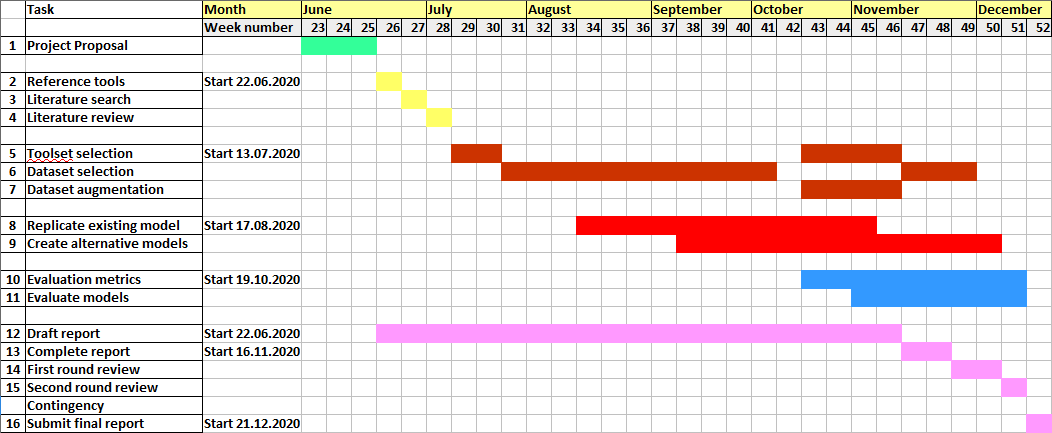
\includegraphics[width=\textwidth]{Figures/Revised-work-breakdown-structure.png}
 \caption{Retrospectively revised project work plan.}
 \label{fig:Revised-work-breakdown-structure} 
\end{figure}

%-----------------------------------
%	Structure of the report
%-----------------------------------

\section{Structure of the Report}

% Chammas - 324 words, no references
The remaining report is structured as follows:
\begin{itemize}
    \item[--] Chapter 2 provides the critical context, project motivation, methods used, literature survey and analysis. It outlines the current state of research with autonomous vehicles deep neural networks, including ConvNets.
    \item[--] Chapter 3 contextualises the broader context of self-driving cars and the technologies pushing research further
    \item[--] Chapter 4 describes results of training networks, together with metrics and video links showing the simulated car models self-driving
    \item[--] Chapter 5 contains a discussion on what objectives were met, what objective was not met and suggested modifications to meet all objectives.
    \item[--] Chapter 6 evaluates and reflects on the project, limitations, contributions and ares for further work.
    \item[--] Appendix \ref{app:rpmi} contains the RPMI project proposal
    \item[--] Appendix \ref{AppendixA-methods} details methods used 
    \item[--] Appendix \ref{AppendixB} contains network architectures used
    \item[--] Appendix \ref{AppendixC-deliverables}  presents tables containing \textit{deliverables} first put forward to project supervisor 
    \item[--] Appendix \ref{AppendixD} contains training logs and notes on gathering results
    \item[--] Appendix \ref{app:source_code_listing} contains listings for original and modified (with attribution) codes used in this project
    \item[--] This document in pdf format and a readme.txt file are submitted in the project submission area. readme.txt file lists SharePoint links for trained models, dataset, source code for training, testing, driving simulator and source code audit files.
\end{itemize}
 
%
\chapter{Context}

\label{Context} 

% LC 43 References

This chapter explains the current state of your topic, in practice and theory. This is the state of the world which you intend to improve, and the state of knowledge on top of which you build your advances and from which you learn knowledge to apply and constraints on your work. So, you will report and analyse what is known about a certain topic, as reported in reference literature and published scientific literature; if you are developing a product, you will need to report about comparable or competing products over which you intend to improve or from which you will obtain ideas; you may need to describe legal or societal situation within which your work takes place; etc.  
  
It is important to demonstrate scholarship, i.e. the ability to read about a subject area in a range of sources, assimilate the material and then discuss it intelligently.  
  
You should demonstrate that you understand what you have read by providing some analysis or commentary in view of the goals of your project: it is not enough simply to provide summaries of what you have read. References should be cited following the Harvard Referencing Style. You must also explain, both in this chapter and, as appropriate, in others, how the results of the studies to which you make reference inform your project work. To gain a passing grade, your report MUST demonstrate adequate engagement with academic literature and any other sources necessary for the work to be well informed.  

% The story we want to tell
% End to end learning - what does it mean
% Describe pipelined methods, contrast and compare to end to end methods

% Datasets and the importance of large public datasets for deep learning
% Synthetic datasets - how these become important as data can be difficult and costly to acquire

%% Prior methods used in image classification, using manual feature extraction

% What is end to end learning?
The properties of multilayer feedforward neural networks as function approximators has been studied extensively, especially in the 1980's . \cite{hornik1989multilayer} rigorously established that standard multilayer feedforward networks with as few as one hidden layer can approximate specific functions provided sufficiently many hidden units are available. while (\cite{cybenko1989approximation}) demonstrated analytically that a feedforward neural network with one hidden layer and any continuous sigmoidal nonlinearity can approximate any function. As such, failures in applications can be attributed to inadequate learning, inadequate numbers of hidden units, or the presence of a  stochastic rather than adeterministic relation between input and target. (\cite{hornik1989multilayer}) state their results do not address the issue of how many units are needed to attain a  given degree of approximation.  



% Maybe a bit of history on SVM, HOG, SURF, etc. Perhaps best in introduction, like how this was a step, where manual feature extraction was used, then came end to end applied to computer vision problems.

% Intro explain term "end to end" - move to intro

% Context - successes in deep convolutional neural networks applied to computer vision problems

% 2. Imagenet - large public dataset \cite{deng2009imagenet}

%% MODELS

% 3. Alexnet - 
% 4. VGG - \cite{simonyan2015deep}
% 5. RESNET \cite{he2015deep}
% 6. Inception \cite{szegedy2014going}

% Then NVIDIA uses a deep convolutional neural networks architecture for end to end driving, i.e. image (raw pixels) in, vehicle control out.

% 1. NVIDIA end to end \cite{bojarski2016end}, DAVE2

% 7. \cite{Su_2019} 
% 8. \cite{zhang2017understanding}

%% However, these networks do have weaknesses, as demonstrated by \cite{Su_2019} in the form of one pixel attacks.
% \cite{zhang2017understanding} % demonstrated that simple depth two neural networks already have perfect finite sample expressivity as soon as the number of parameters exceeds the number of data points as it usually does in practice
%% Such examples question the robustness of deep convolutional neural networks. Especially in the context of one pixel attacks, when small addition of random noise causes the model to completely misinterpret the results, raising questions about generalisation, overfitting and robustness of the deep neural network architectures described.

%% DATASETS

%% 9. Audi dataset https://www.a2d2.audi/a2d2/en/download.html
% \cite{geyer2020a2d2},
%% 10. Ford Multi-AV Seasonal Dataset
% \cite{agarwal2020ford}
%% 11. Udacity
Maybe a bit on how synthetic datasets are used in other domains e.g. https://arxiv.org/pdf/1910.02550.pdf "ClearGrasp:
3D Shape Estimation of Transparent Objects for Manipulation" use of Blender. See section "Learning from synthetic data"

%% Identifying rainy data segments - Amazon Sagemaker 
% 19. \cite{joshi2020amazon}
% Mechanical Turk
% 20. \cite{crowston2012amazon}

%% SYNTHETIC DATASETS
% Cleargrasp
% 12. \cite{sajjan2019cleargrasp}

%% TOOLS -- maybe move tools to METHODS section
%% ROS
% \cite{quigley2009ros}

%% TENSORFLOW
% 13. \cite{abadi2016tensorflow}
%% KERAS
% 14. \cite{chollet2015keras}
%% PYTORCH
% 15. \cite{NEURIPS2019_9015}

% 3D environments
% 3D gaming engines
%% UNREAL - used by INTEL/AUDI/FORD TBC
% 16. \cite{unrealengine}
% user by AIRSIM
% 17. \cite{shah2017airsim}

%% UNITY - used by Udacity
% 18. \cite{haas2014history}

% Blender used to create synthetic datasets
% 21. \cite{rajpura2017object}

%% Public datasets
Kaggle (\cite{kaggle_2020} contains over 50,000 public datasets and 400,000 public jupyter notebooks (\cite{JupyterNotebook2020}), an open-source web application that allows you to create and share documents that contain live code, equations, visualizations and narrative text. Uses include: data cleaning and transformation, numerical simulation, statistical modeling, data visualization and machine learning.

Imagenet is an example of the availability of a computer vision datasets. Public datasets exist for a number of tasks applied to computer vision, such as  
human action and activity recognition (\cite{chaquet2013survey}), agriculture (\cite{lu2020survey}) and hand pose estimation (\cite{li2019survey}).
Intel DevCloud (\cite{IntelDevCloud2020}).

%-----------------------------------
%	BACKGROUND
%-----------------------------------

% A discussion of the proliferation of public datasets applied to machine learning, competitions, code repositiories, libraries is in order to contextualise the availability of data and tools in the context of our research

\section{ImageNet Challenge}

The  ImageNet Large-Scale Visual Recognition Challenge (ILSVRC) (Russakovsky et al., 2014) played an important part in the development of deep neural networks for image recognition. With the exception of DriveNet (NVIDIA end-to-end self-driving ConvNet architecture), all remaining four (AlexNet, GoogleLeNet, VGG and ResNet) were winning entries in the ILSVRC.  

% Interesting compact discussion on various applications of CCN and computer vision and end to end learning with several applications

% https://www.ncbi.nlm.nih.gov/pmc/articles/PMC6539483/ pg

\section{Deep Learning applied to autonomous vehicles}

\subsection{Modular pipeline}

\subsection{End to end learning}



\lipsum[1]

%-----------------------------------
%	DATASETS
%-----------------------------------
\section{Datasets}

TODOS

\begin{itemize}
    \item Itemize / create table of datasets - see surveys
    \item Discuss importance of public datasets
    \item References
\end{itemize}

Advances in computer vision brought about by the Large Scale 

\lipsum[2]

%
\chapter{Methods}

\label{Methods} 

%This chapter describes in detail the methods for whatever activities were necessary for your project – e.g., data gathering, data analysis, requirements analysis, design, implementation, testing/evaluation, etc. Your choice of methods should be discussed and justified in view of the project objectives, and with reference to the pertinent literature. Report not only what methods you applied in generic terms, but what you actually did: sufficient information about dates and details for your reader to understand how you ran your project, rather than just how one could run any similar project.  

%Report in this chapter what you did, not what you produced or found as a 
%result (which goes under Results).  
  
%Note: only use the word ‘methodology’ if you know what it means!  

%% On RELU not actually being differentiable:
%Some of the hidden units included in this list are not actually differentiable %at
%all input points. For example, the rectified linear function g (z) = max{0, z} is not
%differentiable at z = 0. This may seem like it invalidates g for use with a gradientbased
%learning algorithm. In practice, gradient descent still performs well enough
%for these models to be used for machine learning tasks. This is in part because
%neural network training algorithms do not usually arrive at a local minimum of
%the cost function, but instead merely reduce its value significantly,
%Because we do not
%expect training to actually reach a point where the gradient is 0 , it is %acceptable
%for the minima of the cost function to correspond to points with undefined gradient.
%Hidden units that are not differentiable are usually non-differentiable at only a
%small number of points.
% pg 207 Goodfellow
% This section from same book pg 475, maybe better in Context
%Another important push, still ongoing, has been towards end-to-end deep
%learning speech recognition systems that completely remove the HMM. The first
%major breakthrough in this direction came from Graves et al. (2013) who trained
%a deep LSTM RNN (see section 10.10), using MAP inference over the %frame-tophoneme
%alignment, as in LeCun et al. (1998b) and in the CTC framework (Graves
%et al., 2006; Graves, 2012).

% Batch normalization - in the context of preprocessing data for our trainng

% Feedback from Artuz Garcez relevant to Methods section
% The most important thing now is to describe clearly (with the right level of detail - not too much, not too little) the technical process (simulator, adding rain, creating the data, choice of network model and architecture/parameters)

% LC - 14 pages

%%%%%%%%%%%%%%%%%%%%%%%%%%%%%%%%%%%%%%%%%%%%%%%%%%%%%%%%%%%%%%%%%
% DATASETS
%%%%%%%%%%%%%%%%%%%%%%%%%%%%%%%%%%%%%%%%%%%%%%%%%%%%%%%%%%%%%%%%%
\section{Datasets}
Labelled datasets, each image labelled with a steering angle, are required to train self-driving CNNs.
Five datasets are considered Audi (\cite{geyer2020a2d2}), FordAV (\cite{agarwal2020ford}), Kitti (\cite{geiger2013vision}), Udacity (\cite{udacity2020}) and Unity, this last one being synthetic data generated specifically for this project. All provide a labelled dataset in the sense that a steering angle may be obtained for each image. In the case of Udacity simulator and SDSandbox data, the steering angle image label is implicitly stored. IN the remaining datasets, the steering angle may be inferred either by comparing timestamps in plain text log files, or extracting IMU data from rosbag files.

%%%%%%%%%%%%%%%%%%%%%%%%%%%%%%%%%%%%%%%%%%%%%%%%%%%%%%%%%%%%%%%%%
% Keras
%%%%%%%%%%%%%%%%%%%%%%%%%%%%%%%%%%%%%%%%%%%%%%%%%%%%%%%%%%%%%%%%%
\section{Keras}
The Keras (\cite{chollet2015keras}) deep learning API (Application Programming Interface) written in Python (\cite{van1995python}) and in this case acting as a wrapper around the machine learning library Tensorflow (\cite{abadi2016tensorflow}) is used to create, train and test models. The framework allows for designing, compiling and fitting models, saving and loading model weights, early-stopping training, saving best models as training progresses and using models to make predictions. The implementation details are abstracted, making for a clean programming interface, and simple to change hyperparameters such as activation functions, kernel size and stride, learning rate, optimizer and loss metric. 

%%%%%%%%%%%%%%%%%%%%%%%%%%%%%%%%%%%%%%%%%%%%%%%%%%%%%%%%%%%%%%%%%
% tcpflow
%%%%%%%%%%%%%%%%%%%%%%%%%%%%%%%%%%%%%%%%%%%%%%%%%%%%%%%%%%%%%%%%%
\section{tcpflow}
tcpflow (\cite{tcpflowElson2013}, \cite{garfinkel2013passive}) is able to capture data packets, transmitted using the TCP (\cite{rfc793}) host-to-host protocol (which provides a process-to-process communication service) and store the data in a human readable format, such that it may be analysed and debugged. For this study, it is used to reconstruct and record data transmissions between SDSandbox and the prediction engine. A practical example is given in \ref{NetMonDebug}.
% TODO What are we getting from, and why are we using TCP flow
Figure \ref{fig:PredSteeringAnglestcpflowNvidia1} shows a plot of predicted and simulator steering angles. The prediction is for a single image frame sent over the network. As the simulation begins, frames are sent over the network and in this case, captured with tcpflow.

%%%%%%%%%%%%%%%%%%%%%%%%%%%%%%%%%%%%%%%%%%%%%%%%%%%%%%%%%%%%%%%%%
% git version control
%%%%%%%%%%%%%%%%%%%%%%%%%%%%%%%%%%%%%%%%%%%%%%%%%%%%%%%%%%%%%%%%%
\section{Git}
Git (\cite{chacon2014pro}) is a distributed software version control tool, also known as SCM (Source Code Management). It is used in this project to keep track of changes made to software code. A change is recorded through a \textit{commit}, which generates a unique commit hash. By comparing commits it is possible to determine how code was modified between commits. The ability to track such changes is useful to determine code changes over time, and to recall configurations for an experiment to be repeated. An example of the forensic use of Git can be seen in \ref{app_res:36}, to narrow down what code generated a well performing model.

%%%%%%%%%%%%%%%%%%%%%%%%%%%%%%%%%%%%%%%%%%%%%%%%%%%%%%%%%%%%%%%%%
% SDSandbox and the Unity Game Engine
%%%%%%%%%%%%%%%%%%%%%%%%%%%%%%%%%%%%%%%%%%%%%%%%%%%%%%%%%%%%%%%%%

\section{SDSandbox and the Unity Game Engine}
\label{met:sdsandboxAndUnity}
SDSandbox (Self Driving Car Sandbox - \cite{SDSandboxSim}) is a self-driving simulator that uses the Unity (\cite{haas2014history}) game engine to simulate 3d environment car physics, as well as terrain and lighting. SDSandbox adds a user interface with a number of circuits, and functionality to create labelled datasets consisting of images (.jpg files) and steering and throttle data (corresponding .json files). It also allows a model to be driven by a prediction engine. In addition to the Unity simulator (sdsim directory), SDSandbox also provides code (src directory) to train models (train.py) and run inferences (predict\_ client.py). A base model is supplied (models.py) that "uses NVidia PilotNet NN topology", with some modifications.  
  
Setting up the SDSandbox simulator and prediction engine is further detailed in Appendix \ref{RunningCarSimulatorForInference}.

%%%%%%%%%%%%%%%%%%%%%%%%%%%%%%%%%%%%%%%%%%%%%%%%%%%%%%%%%%%%%%%%%
% SD Sandbox and Udacity Driving Simulator Comparison
%%%%%%%%%%%%%%%%%%%%%%%%%%%%%%%%%%%%%%%%%%%%%%%%%%%%%%%%%%%%%%%%%

\section{SD Sandbox and Udacity Driving Simulator Comparison}
\label{met:sdsandbox-udacity-comparison}
Two driving simulators were trialed, an earlier version of Udacity (\cite{UdacityCarSim}) and SDSandbox (see \ref{met:sdsandboxAndUnity}). Both use the Unity game engine. The former had a large user base on account of the accompanying MOOC (Massive Online Open Course), which has since started using the Unreal Engine (\cite{unrealengine}) based Carla (\cite{Dosovitskiy17}) sim (short for simulator). SDSandbox is actively developed for the open source Donkey Car autonomous vehicle (\cite{DonkeyCar2020} and used by the do-it-yourself model-scale autonomous-vehicle community DIY Robocars (\cite{DIYRobocars2020}). The majority of this community uses behavioral learning to train self-driving CNNs (see correspondence with SDSandbox main code maintainer in \ref{corr:ellerbach}).  
 
Both simulators (Figure \ref{fig:UdacitySdSandboxAutonomous}) are equivalent in the sense of acting as a testing environment for self-driving CNNs and also as a training data generator. The difference being SDSandbox is able to generate data using, in addition to manual steering, a self-driving PID (\cite{bennett1993development}) closed loop controller as implemented in PIDController.cs source code file. The process provides feedback to the simulated car, which adjusts itself on the track, based on known geometrical constraints. The feature (option \textit{Auto Drive w Rec}) makes generating training sets less laborious. The manual option (\textit{Joystick/Keyboard w Rec}) being, a simulated car must be manually steered around the track a number of times. The equivalent Udacity sim option being \textit{TRAINING MODE}.

For inference, Udacity and SDSandbox have equivalent modes. The options being   
\textit{AUTONOMOUS MODE} and \textit{NN Control over Network}. Output image sizes are 320x160 and 160x120 respectively. The Udacity sim outputs steering angles to a single comma separated values' (.csv) file, as opposed to multiple .json files. 

\begin{figure}[h!]
\centering
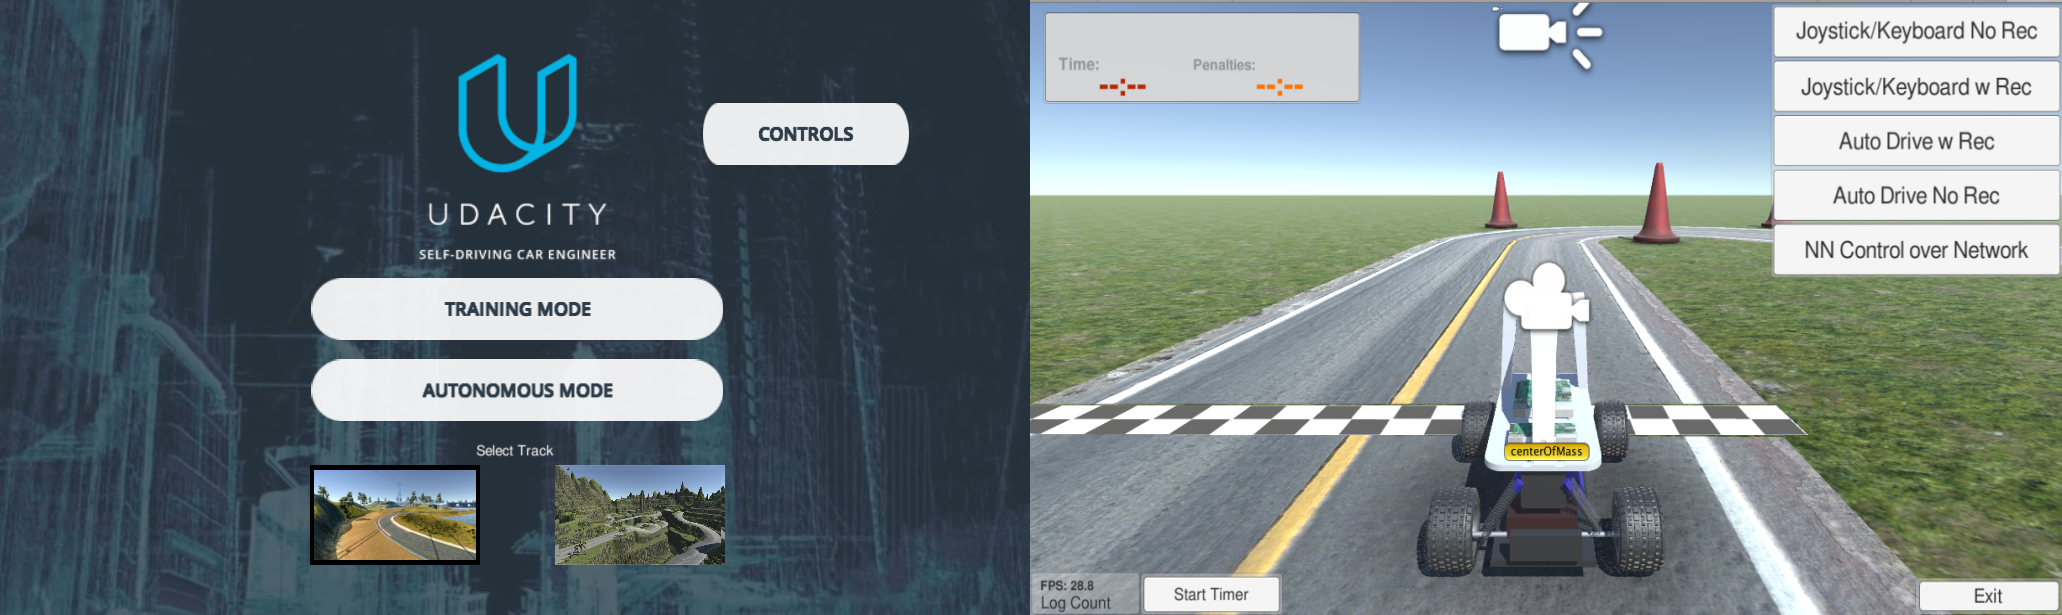
\includegraphics[width=\textwidth]{Figures/UdacitySdSandboxSim.png}
\caption{Left to right: legacy Udacity and SDSandbox Autonomous Driving Simulators}
\label{fig:UdacitySdSandboxAutonomous}
\end{figure}

Appendix \ref{AppendixA-methods} contains further notes on obtaining the source code (\ref{installing-source-code}), running the Unity Hub utility (\ref{running-unity-hub}), generating training datasets (\ref{recording-one-lap} )and running the driving simulator (
\ref{running-driving simulator})

%%%%%%%%%%%%%%%%%%%%%%%%%%%%%%%%%%%%%%%%%%%%%%%%%%%%%%%%%%%%%%%%%
% Generating Synthetic datasets - REPEATED
%%%%%%%%%%%%%%%%%%%%%%%%%%%%%%%%%%%%%%%%%%%%%%%%%%%%%%%%%%%%%%%%%

%\section{Generating Synthetic Datasets}

%\begin{itemize}
%    \item Running SDSandbox in Drive w Rec mode
%\end{itemize}

%SDSandbox has a built-in \textit{Drive w Rec} feature which enables saving of image frames generated while the simulator is running. In addition to the image, a corresponding json encoded file is also saved for every image, containing metadata which includes the reference image file name, and values for steering and throttle of simulated vehicle at the time image frame was recorded. 

%%%%%%%%%%%%%%%%%%%%%%%%%%%%%%%%%%%%%%%%%%%%%%%%%%%%%%%%%%%%%%%%%
% Adding rain to images
%%%%%%%%%%%%%%%%%%%%%%%%%%%%%%%%%%%%%%%%%%%%%%%%%%%%%%%%%%%%%%%%%

\section{Adding rain to images}
\label{methods:AddingRainToImages}
At the core of testing self-driving CNNs in the rain is the ability to add rain to images, never seen before by the network, at inference time.
Rain is added to images using the Automould (\cite{Saxena2017}) library, in turn using opencv-python, a Python port of OpenCV (\cite{mordvintsev2014opencv}), a library for Computer Vision and Machine Learning algorithms. Rain effect is created by adding lines of user defined slant, and random width. The image is then blurred by convolution with a 7x7 normalized box filter (kernel) as shown in equation \ref{eq:blurring-kernel}, taking the average of all the pixels under the kernel area and replacing the central element on the image (\cite{documentationOpenCV2020}) with the result of the convolution operation (Appendix \ref{app:rpmi}, pg 3).

\begin{equation}
\label{eq:blurring-kernel}
    K = \frac{1}{49} \begin{bmatrix} 1 & 1 & 1 & 1 & 1 & 1 & 1 \\ 
    1 & 1 & 1 & 1 & 1 & 1 & 1 \\ 
    1 & 1 & 1 & 1 & 1 & 1 & 1 \\ 
    1 & 1 & 1 & 1 & 1 & 1 & 1 \\ 
    1 & 1 & 1 & 1 & 1 & 1 & 1 \\ 
    1 & 1 & 1 & 1 & 1 & 1 & 1 \\ 
    1 & 1 & 1 & 1 & 1 & 1 & 1 \end{bmatrix}
\end{equation}
The kernel acts as a low pass filter, removing high frequency content (such as noise and edges). The image is then moved from RGB (red, green, blue) to HSL (hue, saturation, lightness) space, where the lightness values are multiplied by 0.7. This has the effect of making the image darker. The process is completed by moving the image back to RGB space. Rain types are \textit{drizzle} (a.k.a. "light", default, code checks for "heavy" and "torrential", any other non-empty string is considered drizzle/light rain), \textit{heavy}, and \textit{torrential}. Slant is defined as an angle in degrees from 0 to plus or minus 20.

% Missing an introduction discussing why this is being done
% The synthetic datasets used contain no rain. To test models with rainy images, rain must % be added. 
% To add rain to the testing images, \textit{Automold Road Augmentation Library} (\cite{Saxena2017}) is used, consisting of a Python module capable of adding rain-like effect to images. 

\begin{figure}[h!]
\centering
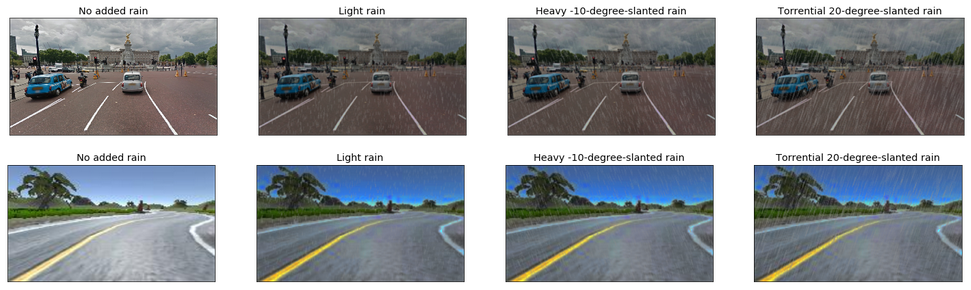
\includegraphics[width=\textwidth]{Figures/AutomoldRain.png}
\caption{Left to right: images}
\label{fig:AutomoldRoadAugmentationLibrary}
\end{figure}

Figure \ref{fig:AutomoldRoadAugmentationLibrary} shows on the top row, a real-life image and on the bottom row, an image created by SDSandbox simulator. The columns from left to right have: no rain added, straight falling (0 degree slant) light, heavy with a -10 degree slant added and torrential rain with a 20 degree slant added.  
During inference (running steering predictions) the image is (in addition to same pre-processing, performed during training time) processed such that it will contain rain never seen before by the network. 
%The outcome is uncertain, given the effect of random noise on CNNs (see section TODO add section with discussion on one pixel attacks), although the flattening effect of the RGB to YUV transformation (see section TODO add section with RGB to YUV discussion) may have a desirable filtering effect.



%%%%%%%%%%%%%%%%%%%%%%%%%%%%%%%%%%%%%%%%%%%%%%%%%%%%%%%%%%%%%%%%%
% Data Augmentation and Pre-Processing
%%%%%%%%%%%%%%%%%%%%%%%%%%%%%%%%%%%%%%%%%%%%%%%%%%%%%%%%%%%%%%%%%

\section{Data Augmentation and Pre-Processing}
\label{met:data-aug-pre-proc}
% Missing an introduction on why this is important
As discussed in \ref{Context}, data augmentation can be used to reduce overfitting, by increasing the amount of training data. The data augmentation library used in this study is adapted from \cite{Naoki2016}. Critical to the design of computer vision CNNs is the geometry of the input image. The adapted augmentation library (Augmentation.py) first resizes the image to the expected size of acquired image in the original network design. This enables code re-usability, where different networks, using different image sizes can be tested using the same code. 
Increase by a factor of 1.6 in this study.
%For the NVIDIA baseline model, assumed image capture size is 320x160 pixels, and the 200x66 pixel image presented to network is a crop containing road and excluding horizon. 
The sequence shown in figure \ref{fig:augpreproc} presents image array sizes at every step, from top left to bottom right, the image is loaded and resized (to 320 width x 160 height pixels in this case), augmented with random horizontal flip (with corresponding steering negated), random horizontal shifts (with steering adjusted by adding or subtracting 0.002 degrees per shifted pixel, random addition of shadows and random modification of brightness, concluding the augmentation part.
\begin{figure}[h!]
 \centering 
 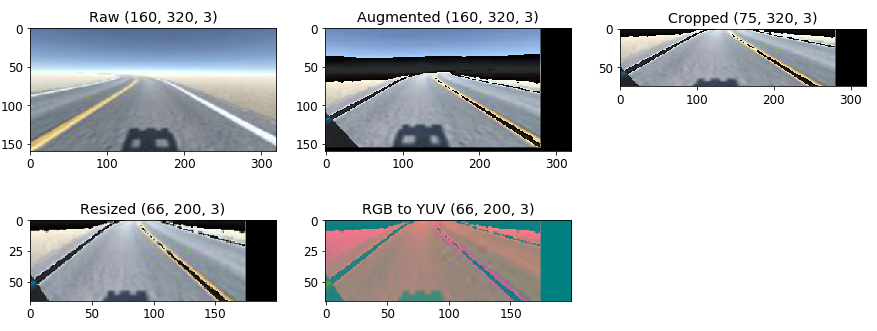
\includegraphics[width=\textwidth]{Figures/AugmentationPreProcessing.png}
 \caption{Stages of image augmentation (DriveNet and NaokiNet image geometries) and pre-processing with corresponding image array dimensions of each step}
 \label{fig:augpreproc}
\end{figure}

For the pre-processing part, the image is then cropped to remove car and horizon, resized to the dimensions determined by network design (200x66 pixels for baseline network). Crop parameters (amount of image to be removed from top and bottom sections) is network dependant and set in a configuration file (conf.py). In the example shown, 25 rows of pixels were removed from the bottom and 60 rows of pixels were removed from the top, resulting in a 320 x 75 pixel image. The image in then resized to the geometry to be presented to network, in this case 200 x 66, which is the geometry used by NaokiNet and DriveNet. Finally the image is moved from RGB to YUV space. In the RGB scheme, each pixel is represented by three channel intensities of red, green and blue. In YUV, also referred to as YCbCr (\cite{maller2020}) space, each pixel is represented by Y (luma), U (Cb - luminance value subtracted from red channel) and V (Cr - luminance value subtracted from red channel). It is a "lossy" process which degrades the data, and originally developed for colour to black and white television backward compatibility. Moving the image from RGB to YUV space has been demonstrated to give "better subjective image quality than the RGB color space", being better for computer vision "implementations than RGB due to the perceptual similarities to the human vision" (\cite{podpora2014yuv}). This scheme was used in Dave, the Autonomous off-road vehicle (\cite{lecun2004dave}) which used end to end learning.





% Prior to presenting pixel colour channel values to the network, a number of pre-processing steps have become standard with neural network classifiers and regressors applied to computer vision.

% maybe move to appendix or results, explaining here for now

%\section{Data Augmentation}
%To avoid overfitting, the data is augmented by: cropping the %image to a height band that excluded horizon and car shadow, %resized to required model input size, converted from RGB to YUV, 
% get images from http://localhost:8890/notebooks/augument.ipynb

% \section{Training a model}

\section{Identifying rainy images with Amazon Mechanical Turk}

Amazon Mechanical Turk \cite{crowston2012amazon} is an online marketplace where jobs can be outsourced using the \textit{crowsourcing} model  (\cite{vukovic2009crowdsourcing}) which delivers a scalable workforce that may be adjusted in size as required. Mechanical Turk has been referred to as \textit{artificial artificial intelligence} (\cite{dai2011artificial}) where a task requiring human intelligence level, such as labelling an image, can be assigned to a real person, in lieu of writing  a computer algorithm capable of doing so. Mechanical Turk, launched in 2005, was instrumental in labelling the Imagenet (\cite{deng2009imagenet}) dataset which lead to advances in computer vision image recognition with a number of deep (TODO explain "deep" at some point) network architectures ( \cite{krizhevsky2012imagenet}, \cite{he2015deep}, \cite{szegedy2014going} and \cite{simonyan2015deep}). 

\begin{figure}[h!]
 \centering 
 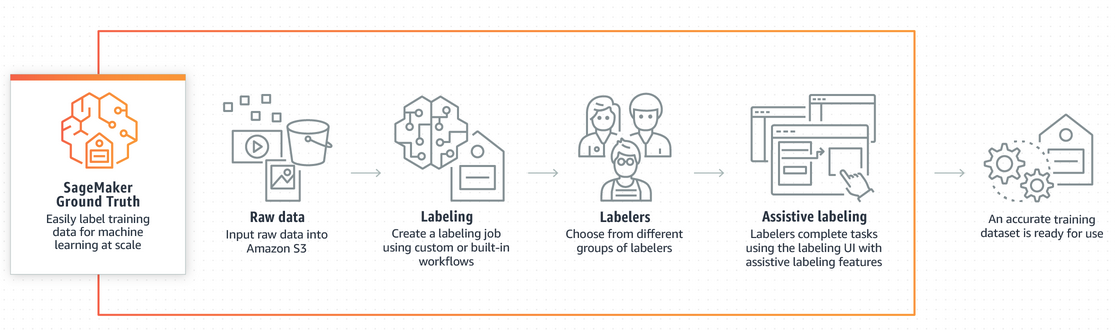
\includegraphics[width=\textwidth]{Figures/SageMakerGroundTruth.png}
 \caption{Amazon SageMaker Ground Truth workflow: a dataset is placed on Amazon S3, labeling job is created, workers label data using a labeling user interface resulting in a labeled dataset}
 \label{fig:amazon-ground-truth}
\end{figure}

For this study Amazon SageMaker Ground Truth (\cite{SageMakerGroundTruthDocumentation2020}) was used. It is a wrapper for Mechanical Turk, and facilitates the process of setting up the image labelling job, especially the UI (user interface) that the labeler workforce must used.  
The aim here is to find segments of real life footage that may contain rain. The Ford AV (\cite{agarwal2020ford}) has sections labeled as "cloudy" so may contain rain. 100 images, chosen at regular intervals, the expectation being this may help narrow down the location of rainy images, if any. To test the accuracy of the service, 5 images with rain are added to the dataset. The expectation being labels for these 5 images will be "rain". 
% https://us-east-2.console.aws.amazon.com/sagemaker/groundtruth?region=us-east-2#/labeling-jobs/create
The unlabelled dataset is stored on AWS S3 (\cite{AmazonS3Documentation2020}). An "Image Classification (Single Label)" "Task type" is chosen, i.e. workers will verify if the proposed label "Rainy image" is correct. The process workflow is shown of Figure \ref{fig:amazon-ground-truth}.




%%%%%%%%%%%%%%%%%%%%%%%%%%%%%%%%%%%%%%%%%%%%%
% NVIDIA END TO END LEARNING
%%%%%%%%%%%%%%%%%%%%%%%%%%%%%%%%%%%%%%%%%%%%%
\section{NVIDIA \textit{End to End Learning for Self-Driving Cars} Network Architecture}

The NVIDIA network (\ref{NVIDIA_baseline}) architecture, also known as \textit{PilotNet} (\cite{bojarski2020nvidia}) is the baseline self-driving architecture used in this study. This comprises 3 (RGB channel) x 66 (height) x 200 (width) size input layer corresponding to an image presented to network. The input layer is followed by: a normalization layer generating a 3 channel 66 x 200 layer, a 24 5x5 kernel convolutional layer generating 31x98 feature maps, a 36 5x5 kernel convolutional layer generating 14x47 feature maps, a 48 5x5 kernel convolutional layer generating 5x22 size feature maps, a 64 3x3 kernel convolutional layer generating 3x20 size feature maps, a 64 3x3 kernel generating 1x18 size feature maps, a 1164 neuron flattened layer fully connected to a 100 neuron layer, fully connected to a 50 neuron layer, fully connected to a 10 neuron layer, fully connected to a one neuron output layer.  
The first 3 convolutional layers have stride equal 2 and the last 2 convolutional layers have stride equal 1. Padding is equal to zero, resulting in smaller feature maps with every convolutional layer.
The size of feature maps generated by each convolutional layer is determined with equation \ref{eq:feature_map} as described in \cite{dumoulin2018guide}:
\begin{equation}
    \label{eq:feature_map}
    n_{out}= \Big\lfloor\frac{n_{in} + 2p -k}{s} \Big\rfloor +1
\end{equation}
where $n_{out}$ is output size of convolved feature map, $n_{in}$ is input size of image or feature map, $p$, $k$ and $s$ are padding, kernel and stride size respectively.  
 
For example, to determine size of feature maps in the first convolutional layer $n_{out}=\lfloor(66+(2\times0)-5)/2\rfloor)+1=31$, $n_{out}=\lfloor(200+(2\times0)-5)/2\rfloor+1=98$. The Keras (\cite{chollet2015keras}) machine learning framework is used to build the model. The calculation for number of trainable parameters (weights) in a convolutional layer is given in equation \ref{eq:trainable_params}:
\begin{equation}
    \label{eq:trainable_params}
    n_p= m \times n \times  d \times k + d
\end{equation}
where $m$ and $n$ are the convolutional kernel dimensions, $d$ is the number of feature maps in the current layer and $k$ is the number of feature maps in the previous layer. Note $d$ is added to account for \textit{bias} term. For example, the number of trainable parameters for the first convolutional layer in \ref{NVIDIA_baseline} is given by $n_p = 5 \times 5 \times 24 \times 3 + 24 = 1,824$. The number of trainable parameters in a fully connected layer is given by equation \ref{eq:trainable-parmas}:
\begin{equation}
    \label{eq:trainable-parmas}
    n_p= m \times n + n
\end{equation}
where $m$ is the number of inputs in previous layer and $n$ is number of neurons in current layer. Note second term $n$ is added to account for \textit{bias} term. For example, for the first fully connected layer in \ref{NVIDIA_baseline} the number of parameters is given by $n_p = 1164 \times 100 = 1,342,092$, where the inputs are values from previous flattened layer, that is, a vectorized representation of the last convolutional layer feature maps.  
The total number of trainable parameters generated by Keras is 1,595,511. This does not agree with the total given by \cite{bojarski2016end}, their "network  has  about (...) 250 thousand parameters". Total memory required to store parameters assuming 32-bit float data type, is 6MB given by $1,595,511 \times 4 \div 1,024 \div 1,024$.

Since the NVIDIA model is based on work by \cite{krizhevsky2012imagenet}, "dropout" (\cite{hinton2012improving}) is assumed to have been used, with 50\% dropout probability on every layer.  
Dropout removes neurons randomly and helps prevent overfitting, where a model performs well on training data and poorly on testing data, by preventing co-adaptation, resulting in neurons that can detect useful features in the multitude of contexts it must operate, and help the network produce the correct answer.
As per correspondence with co-author(\ref{corr_with_authors} additional training hyperparameters are MSE (loss function) 
adadelta (optimizer), "learning rate: 1e-4 (but not really used in adadelta)" and 0.25 dropout.
Additional assumptions on training include: 128 example batch size, weights initialized from a zero-mean normal distribution with standard deviation 0.01 and biases mostly initialized to 1 as per \cite{krizhevsky2012imagenet}, which applied to this baseline architecture initializes all biases to 1, except in convolutional layers 1 and 5, where biases are initialized to 0. Details in source code src/models.py, nivia\_ baseline function.  


% TODO need to incorporate section 5    Details of learning of Krizhesvky et al i.e.
%We trained our models using stochastic gradient descent with a batch size of 128 examples, momentum of 0.9, andw eight decay of 0.0005. ETC

% Since the weights are not initialized properly and groups of neurons end up in the same local minima, according to their (similar) initialization.
% To overcome this, you could use dropout / drop connect to break symmetry.
% https://stats.stackexchange.com/questions/181264/how-does-co-adaptation-occur-in-deep-neural-nets

% NB no reference to "Alexnet" in original or NVIDIA articles - clean up required.
%For example, in the classic Alexnet (\cite{krizhevsky2012imagenet}) architecture, with input %image size 224x224, kernel size 11, padding equal zero and stride = 4, the resulting feature %map size in the first convolutional layer is 55x55. 
%Alexnet has an input layer with dimensions 224x224x3, where 3 is the number of channels (RGB %image), the second layer has dimensions 55x55x48, the third convolutional layer has %dimensions 27x27x128 and so on. This is typical of deep network architectures, decreasing %feature map sizes with increasing number of channels as network depth increases.

%%%%%%%%%%%%%%%%%%%%%%%%%%%%%%%%%%%%%%%%%%%%%
% Deep Convolutional Neural Network Models
%%%%%%%%%%%%%%%%%%%%%%%%%%%%%%%%%%%%%%%%%%%%%
\section{Alternative CNN Models}

In addition to PilotNet, two other designs are considers, one supplied with the SDSandbox framework, and referred to in this text as \textit{TawnNet}, the other supplied by \cite{Naoki2016} and referred to in this text as \textit{NaokiNet}. These can be seen as simplified variants of PilotNet, and a good starting point, as the original NVIDIA paper makes available no public source code. These architectures are shown in \ref{arc:nvidia1} and \ref{arc:nvidia2} respectively. TawnNet being used as-is and NaokiNet being modified after TawnNet to include 5 dropout layers (originally only one after the last convolutional layer, with dropout set to 0.5) after each convolutional layer, with dropout set to 0.1. Additionally, the number of feature maps in the second convolutional layer was changed from 36 to 32.

%%%%%%%%%%%%%%%%%%%%%%%%%%%%%%%%%%%%%%%%%%%%
% TRAINING ENVIRONMENTS
%%%%%%%%%%%%%%%%%%%%%%%%%%%%%%%%%%%%%%%%%%%%

\section{Training Environments}
% TODO add the "pickle" model
Three training environments are used, a local workstation running Ubuntu 18.04 with 31GB RAM and 12-core CPU, City University's shared Camber (City University cloud server) running Ubuntu 16.04 with 125G RAM and 48-core CPU and the Intel's shared DevCloud running Ubuntu 18.04 with 250G RAM and 80-core CPU. None have GPU processors.

% number of processors
% $ cat /proc/cpuinfo | grep processor | wc -l
% OS
% $ cat  /etc/os-release
% Available memory
% $ free -h

%u52850@s099-n009:~$ cat /proc/cpuinfo | grep processor | wc -l
%80
%u52850@s099-n009:~$ cat  /etc/os-release
%NAME="Ubuntu"
%VERSION="18.04.2 LTS (Bionic Beaver)"
%ID=ubuntu
%ID_LIKE=debian
%PRETTY_NAME="Ubuntu 18.04.2 LTS"
%VERSION_ID="18.04"
%HOME_URL="https://www.ubuntu.com/"
%SUPPORT_URL="https://help.ubuntu.com/"
%BUG_REPORT_URL="https://bugs.launchpad.net/ubuntu/"
%PRIVACY_POLICY_URL="https://www.ubuntu.com/legal/terms-and-policies/privacy-policy"
%VERSION_CODENAME=bionic
%UBUNTU_CODENAME=bionic
%u52850@s099-n009:~$ free -h
%              total        used        free      shared  buff/cache   available
%%Mem:           250G        1.4G        248G        2.1M        276M        247G
%Swap:          1.9G          0B        1.9G
%u52850@s099-n009:~$

%%%%%%%%%%%%%%%%%%%%%%%%%%%%%%%%%%%%%%
% TRAINING
%%%%%%%%%%%%%%%%%%%%%%%%%%%%%%%%%%%%%%
\section{Training}
Training can be performed in any of the environments once all the required python modules are installed and data have been downloaded or created. In case of Camber and the Intel DevCloud, jobs are batched. In the local environment SDSandbox python training scripts run from the command line.  
The neural networks in this project are trained using the Adam optimizer, learning rate set to 0.0001 except where noted, batch size of 64, 

%%%%%%%%%%%%%%%%%%%%%%%%%%%%%%%%%%%%%%
% EVALUATION
%%%%%%%%%%%%%%%%%%%%%%%%%%%%%%%%%%%%%%

\section{Evaluation}

The evaluation can be performed qualitatively using a simulator as described in \ref{met:sdsandbox-udacity-comparison} to observe the simulated vehicle self-driving with respect to oversteering and understeering, crashes providing pass/fail metric.

The proposed quantitive evaluation metric is \textit{goodness-of-steer}. In equation     \ref{eq:goodness_of_steer}:

\begin{equation}
    \label{eq:goodness_of_steer}
    g_s(p,g) = \frac{\sum_i^N \lvert p(i)-g(i) \rvert }{N} \times n_c
\end{equation}
where $p,g$ are prediction and ground truth arrays,  $N$ is the number of predictions and $n_c$ is the normalization constant (25 in example shown, 1 for values not normalized), which in this case is the maximum steering angle for the SDSandbox simulated vehicle. In plain english, $g_s$ is defined as the sum of the absolute value of the difference between prediction and ground truth values, divided by the number of predictions multiplied by a normalization constant, that is the steering error average over all predictions. 
%\begin{equation}
%    \label{eq:g(x,y)}
%    g(x,y) = \matchcal{H} Stopped here
%\end{equation}
TODO read up on noise models (Gonzalez)
% https://ebookcentral.proquest.com/lib/city/reader.action?docID=5573669


% From https://en.wikipedia.org/wiki/Noise_(electronics)
%In communication systems, noise is an error or undesired random disturbance of a useful information signal. The noise is a summation of unwanted or disturbing energy from natural and sometimes man-made sources. Noise is, however, typically distinguished from interference,[a] for example in the signal-to-noise ratio (SNR), signal-to-interference ratio (SIR) and signal-to-noise plus interference ratio (SNIR) measures. Noise is also typically distinguished from distortion, which is an unwanted systematic alteration of the signal waveform by the communication equipment, for example in signal-to-noise and distortion ratio (SINAD) and total harmonic distortion plus noise (THD+N) measures.

%While noise is generally unwanted, it can serve a useful purpose in some applications, such as random number generation or dither. 

%% Udacity
%% see https://arxiv.org/pdf/1912.05440.pdf
%% for discussion on using rmse as error metric - NB This relates to training a network, not the analysis of image noise.

%%%%%%%%%%%%%%%%%%%%%%%%%%%%%%%%%%%%%%%%%%%%%%%%%%%%%%%%%%%%%%%%%
% CREATING VIDEOS
%%%%%%%%%%%%%%%%%%%%%%%%%%%%%%%%%%%%%%%%%%%%%%%%%%%%%%%%%%%%%%%%%
\section{Creating Videos}
Videos are used in this project for qualitative analysis as well as documentation. Three methods are used to create videos. The first is with the Kazam (\cite{Kazam2020}) desktop screen capture utility, which records the contents of a given display monitor. This generates video captures such as shown in Figure \ref{fig:SimTCPPred}, noting the video contains only one frame, and the three images shown in the figure represent different parts of the video. The second method was developed for this project (MakeVideo.py) and consists of parsing tcpflow logs, extracting images and predicted steering angles and creating a "side-by-side" video of the simulator being driven by the prediction engine, next to the re-created processed image presented to the network, generating video captures such as shown in Figure  \ref{fig:20201120171015_sanity_sim_network}. Examples of running the script to generate videos can be seen in a number of documented "runs", for instance \ref{app_res:36} and \ref{app_res:36}. The third method was also developed for this project (RecordVideo.py). It creates a recording at inference time with up to 3 (in case of added rain) side-by-side images in a single video. An example is shown in Figure \ref{fig:youtube20201207091932nvidia1lightrainmult_4_h5}, where most parameters (network name, rain type, predicted steering angle) are generated dynamically, and the "Intensity Multiplie" (sic) value is set in SDSandbox, hardcoded in predict\_ client.py, this python script then committed to git repository and a record of commit hash, tracking the code state at the moment recording was made, is kept in appendix \ref{res:training_and_testing_log} to make results repeatable. The concept of altering intensity multipliers to simulate glare on wet roads is in response to a suggestion by this project's supervisor (see correspondence with supervisor \ref{met:corr_arthur_2}). Examples of running the prediction engine to record can be seen in various runs, including \ref{app_res:51} and \ref{app_res:52}.

%%%%%%%%%%%%%%%%%%%%%%%%%%%%%%%%%%%%%%%%%%%%%%%%%%%%%%%%%%%%%%%%%
% Data plots
%%%%%%%%%%%%%%%%%%%%%%%%%%%%%%%%%%%%%%%%%%%%%%%%%%%%%%%%%%%%%%%%%
\section{Steering data plots}
Another important analysis tool are steering data plots, be it steering angle labels for an image or predictions returned by a Keras model for an image. In this project plots are created with the python matplotlib.pyplot and seaborn modules, using both jupiter notebook such as GetSteeringAnglesFromtcpflow.ipynb and python scripts such as result\_ plots.py and steerlib.py ( \ref{app:source_code_listing}).


\chapter{Results}
% LC 25pgs
\label{Results} 

This chapter presents the outputs that you produced, by applying the methods that you have selected, including e.g. analysis, design, prototyping, experimental work, evaluation, etc.  
  
How you report these results will depend on the nature of the work. It may be helpful to divide them into basic data (e.g., for a project that developed a software product, requirements specification, test data, etc.) and analysis of the data (e.g. statistical analyses, evaluation analyses, etc.). Remember that you are informing the reader of what you have produced and found and emphasising the interesting parts, so summarising at the end of each major section is useful.  
  
It is usually very helpful for the readers to include graphics and diagrams, for instance to clarify software design or requirements, identify key trends and relationships in empirical data, etc. If you do so, be sure to refer to these figures in the text and use them as evidence to support what you are explaining or arguing; and be sure that your figures are well designed and clearly presented – do not just use default settings of the software you are using in producing them.  
  
It is essential that you identify clearly what you accomplished or produced yourself, as opposed to what existed before you started your individual project or was provided by others. For instance, some projects build new software on top of an existing code base, add new data to an existing body of data, or are executed by a student as a member of a team. It is essential to indicate what parts of the activities and results which you report are your own work. If this is left unclear, the markers are instructed not to give credit for work that they cannot attribute to you. Ambiguity would attract penalties for poor academic practice, with delays caused by any investigation (deception would be treated as academic misconduct, of course, which may lead to expulsion).

%-----------------------------------
%	Network training
%-----------------------------------



\section{Network training}

% write up, label runs and make reference
The first working model (able to successfully self-drive around the Generated Track

% probably best to more this to results section and reference here
\begin{verbatim}
# data: genRoad (log2 renamed)
# commit: 1ad187d4bff5b6936c065a1aaa15a654ef4d368c
$ python train.py --model=sanity --outdir=../trained_models
\end{verbatim}
this will create the a model in trained\_output/sanity/20201120184912\_sanity.h5
and run as per procedure described in (TODO add reference).



\begin{verbatim}
# data: genRoad (log2 renamed)
# commit: 1ad187d4bff5b6936c065a1aaa15a654ef4d368c
$ python train.py --model=sanity --outdir=../trained_models
\end{verbatim}
this will create the a model in trained\_output/sanity/20201120184912\_sanity.h5
and run as per procedure described in (TODO add reference).

\subsection{Modifications to original source code}
Models are trained with code written in train.py, models.py and conf.py. This code has been modified from the original. To compare changes a git diff can be copying the original code over the source code used in this project and performing a "git diff"
\begin{verbatim}
# clone repository for dissertation
$ git clone https://github.com/dsikar/sdsandbox
# clone original
$ git clone https://github.com/tawnkramer/sdsandbox sandbox_orig
# copy original over dissertation
$ cp sandbox_org/src/* sdsandbox/src
# compare
$ cd sdsandbox 
$ git diff
\end{verbatim}


Starting with the NVIDIA baseline, a number of hyperparameters were trialed. The initial setup failed to generate usable models. 
The table below presents training results for best trained models.

% training with one parameter

\section{Simulated self-driving car}

Using the baseline neural network architecture as described in 
Models trained with no image pre-processing, did not perform well, leading to cars driving off the road, as shown in Fig.  sequence.

% data gathered on Robot Racing League track
We gathered 10 laps of data on the Robot Racing League track, with maximum speed set to 2.1, proportional control set to 16 and differential set to 77. Maximum steer was set to 25 (degrees). Corresponding to 12778 .jpg image files and the same number of  .json files, containing corresponding throttle and steering angle values recorded at the moment image was saved by simulator. This can be seen in the calls to Update() and SaveCamSensor functions in  
\begin{verbatim}
./Assets/Scripts/Logger.cs
\end{verbatim}

\section{Generated Track performance}


The $G_s$ (goodness-of-steer) model performance score, was obtained by recording one full lap and comparing steering angles with model predictions.

\section{Datasets}

The following training datasets were generated:

Origin  Directory   Number of files Comment
SDSandbox   unity/smallLoopingCourse/log/* 34443 from small\_looping\_course
SDSandbox   unity/warehouse/*   41126 From Warehouse course
SDSandbox   unity/smallLoop/*   45422   From small\_looping\_course
SDSandbox   unity/roboRacingLeague/* 12778 From "Robot Racing League" course
SDSandbox   unity/log\_sample   25791   From small\_looping\_course
SDSandbox   unity/genRoad 280727 From "Generated Road" course



Following the list of data deliverables (\ref{Deliverables-Datasets}) the Udacity data consisting of two files 

\subsection{Locating rainy sections with Mechanical Turk}
For Mechanical Turk, the data that looked most promising was Ford V2 Log 1 and V3 Log 1, both described as "freeway, overpass, bridge, cloudy". We drew 50 images uniformly from each log and added 5 images with rain that were expected to be labelled as such. The 105 images were then added to a SageMaker Ground Truth job. The platform works as a wrapper around Mechanical Turk as it facilitates the creation of user interfaces (Figure \ref{fig:MechTurkCreateJob})
% rainy files created with automold/RainyImagesDissertationPlot.ipynb
\begin{figure}[h!]
\centering
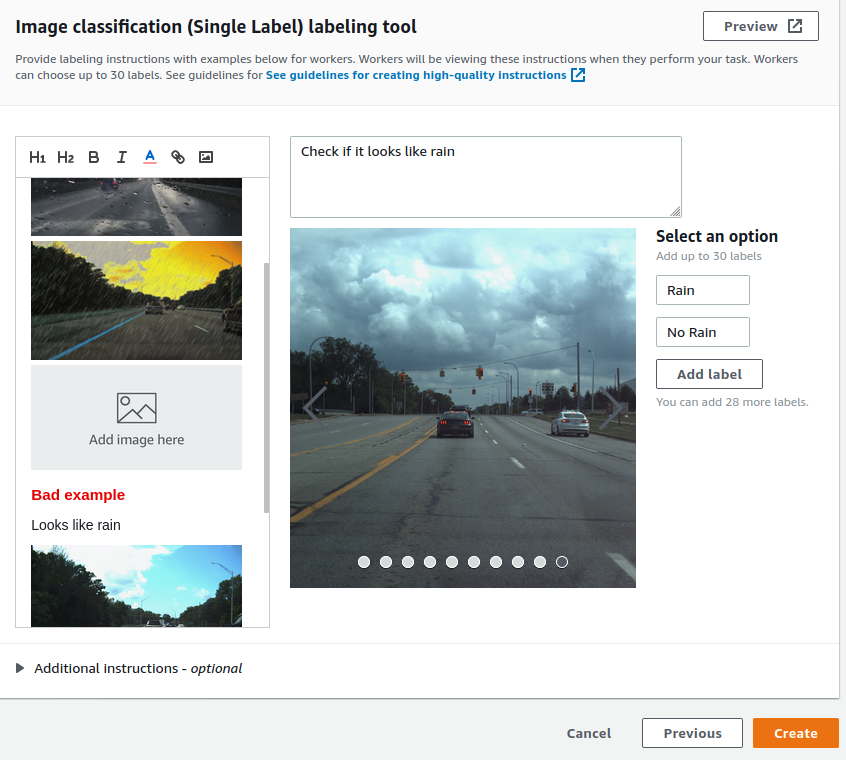
\includegraphics[width=10cm]{Figures/MechTurkCreateJob.png}
\caption{The SageMaker Ground Truth user interface template with two labels ("Rain", "No Rain"), the image to be labeled and examples of correct and incorrect classifications.}
\label{fig:MechTurkCreateJob}
\end{figure}
Labeling tasks are classified as low, medium and high complexity. The prices range from \$0.012 for a low complexity task, with a 5 second estimate to complete, to \$1.20 for a high complexity task with a 3.5 minute estimate to complete.
The task can be configured with an output for time taken by a worker on a single task, the lowest time interval being one minute.
There is also an option to assign more than one worker per dataset object, on account that it can help increase the accuracy of the data labels.
The task was created with the most basic options of one worker, a \$0.012 price per task, a one minute timeout and remained live for 12 hours. 
The images were labelled by Mechanical Turk workers and results made available in a json encoded file (datasets/mechanical-turk/2020-11-21\_22 45 37.json) showing no images had been labeled as "Rain". The assumption then being there are no sections containing rain in the dataset. The Automold library added rain images were also labeled as "No Rain". Figure \ref{fig:MechTurkLabeledImages}
\begin{figure}[h!]
\centering
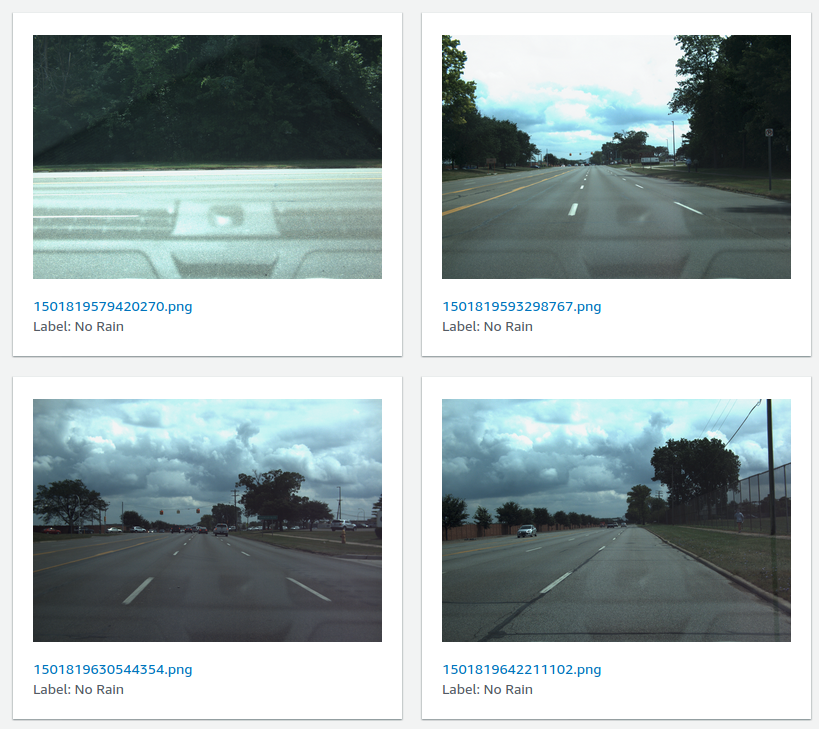
\includegraphics[width=10cm]{Figures/MechTurkLabeledImages.png}
\caption{The SageMaker Ground Truth labeled images detail on Labeling Job Summary page}
\label{fig:MechTurkLabeledImages}
\end{figure}

%-----------------------------------
%	Network running
%-----------------------------------

\chapter{Discussion}

\label{Discussion} 

%This chapter examines your results in comparison with your objectives, and then in the wider perspective of other theoretical and applied work relevant to your project, as covered in your review in Chapter 2. For instance, for a software product you will discuss how well it satisfies the user needs that it addresses, its performance and dependability, aspects of design, implementation or assessment that have proved good choices or that instead you would change if you were to repeat the project knowing what you now know. For novel research results or any other knowledge obtained through the project, you will discuss your confidence in the results, their validity, scope and their generalisability. What are the implications of what you have found out? Do you have any recommendations as a result?

%\section{Andrew Ng CNN complexity table - number of parameters}
%Convolutional Neural Network Examples    
  
%See C4W1L10 CNN Example 10m15s  

%Another interesting performance metric, "While ResNets have definitely improved over Oxford’s VGG models in terms of efficiency, GoogleNet seems to still be more efficient in terms of the accuracy / ms ratio.", basically how much accuracy is achieved with respect to training time, this could provide a single magnitude.

% Discuss Mechanical Turk and Automold images being labeled as No Rain

examine results in comparison with objectives
\begin{itemize}
    \item[--] Game engine - able to support experiments?
    \item[--] Datasets
    \item[--] Image augmentation
    \item[--] Training models
    \item[--] Workflow
    \item[--] Evaluation metric
\end{itemize}
Discuss:
\begin{itemize}
    \item[--] Validity
    \item[--] Scope
    \item[--] Generalisability
    \item[--] Implications
    \item[--] Recommendations
\end{itemize}
Havoc created by outliers in genRoad. 20201206211122\_ nvidia1.h5 performs well on genRoad (where is was trained) but not well on genTrack. Models trained on genTrack also do well on genRoad. Why?
%
\chapter{Evaluation, Reflections and Conclusions}

\label{Eval} 

This chapter should evaluate the project work as a whole. Here the original choice of objectives, the literature examined, the methods used, the planning, etc. are all reviewed to see what has been achieved by undertaking the project. There may be a summary of general conclusions drawn from the work done, highlighting the particular contribution of your project. You should also consider the implications of these conclusions. Discuss any proposals that you might make for further work, having discovered what you now know. It is also important to include a reflective section covering what you have learned from the project process. What would you do differently if you were to start again, knowing what you now know? Your report MUST include adequate Evaluation, Reflections and Conclusions to gain a passing grade.  

Here would be a good place, perhaps, to discuss "Understanding deep learning requires rethinking generalization", Zhang ICLR 2017, on deep models fitting random data (noise) perfectly.

The absence of good quality labelled datasets has been cited (TODO citation needed) as a hindrance to the development of good models (TODO need to insert in CONTEXT section "the term model hereafter, refers to a either a neural network architeture, or a trained model capable of making predictions given an input). It is ironic that the availability of good quality labelled models, such as Imagenet, led to the improvement in image classification models, which in turn may curb the need to use Mechanical Turk. This could perhaps form part of the wider discussion on automated workforce replacing human workforce and the social implications therein.  

%----------------------------------------------------------------------------------------
%	BIBLIOGRAPHY
%----------------------------------------------------------------------------------------

\printbibliography[heading=bibintoc]

%----------------------------------------------------------------------------------------

%----------------------------------------------------------------------------------------
%	THESIS CONTENT - APPENDICES
%----------------------------------------------------------------------------------------


\appendix % Cue to tell LaTeX that the following "chapters" are Appendices

% Appendix page numbering
\pretocmd{\chapter}{%
  \clearpage
  \pagenumbering{arabic}%
  \renewcommand*{\thepage}{\thechapter\arabic{page}}%
}{}{}

% Include the appendices of the thesis as separate files from the Appendices folder
% Uncomment the lines as you write the Appendices

\begin{appendices}
% TODO COMMENT ALL IN FOR FINAL COMPILE
%% Appendix 0 - RPMI Project

\chapter{RPMI Project Proposal Proposal} % Main appendix title

% RPMI Project Proposal to be included. 
\includepdf[page={1-9}]{Sikar_D_RPMI_Task2}
%% Appendix A
\label{AppendixA-methods} % For referencing this appendix elsewhere, use \ref{AppendixA}
\chapter{Methods} % Main appendix title

Procedures used to set up experiments are detailed in this appendix.

\section{Generating graphs}

Two graphs are used, steering angle histograms and steering angle plots. A set of functions have been written for this purpose in steerlib.py. For example to generate a histogram of steering angles from a 

\section{Network architectures for future reference}

\subsection{ResNet}

Discuss the concept of "residuals". ResNet makes use of skip-connections (spelling), these "network architecture
designs (e.g., skip connections) produce loss functions that train easier", producing smoother loss surfaces (\cite{li2017visualizing})  
The "Degradation problem itself stems from the fact that it is easier to learn 0 than to learn 1"   https://www.youtube.com/watch?v=jio04YvgraU
"if an identity mapping were optimal, it would be easier to push the residual to zero than to fit an identity mapping by a stack of nonlinear layers" \cite{he2015deep}.  
Explain what variation A, B or C we will be using (zero padding, weights * x, etc.  
"Essemble" of ResNets was used.  
18 layers seems to be a threshold, beyond that, training becomes difficult. Skip connections make deeper networks, i.e. networks with more layers, easier to train compared to networks without skip connections.  
Another wording, deeper neural networks (i.e. layer count equal or greater than 20) become increasingly difficult to train, generating poorer accuracy than deep networks with less than 20 layers. This is known as "degradation problem" (citation needed). Skip connections make deeper architectures easier to train, by smoothing the loss function.

\subsection{GoogleLeNet}

This network (\cite{szegedy2014going}) was the winning entry in the ILSVCC 2014 Classification Challenge. It uses the LeNet-5 (\cite{Lecun98gradient-basedlearning}) model as a starting point, following the now traditional design of ConvNets with the addition of \textit{Inception} modules as introduced by \cite{lin2013network} in the \textit{Network in Network} model.

\begin{figure}[ht]
 \centering 
 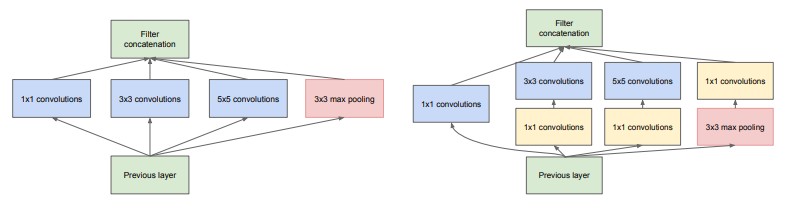
\includegraphics[width=\columnwidth]{Figures/InceptionModules.png}
 \caption{Inception naive (left) and dimension reduction model (right)}
 \label{fig:inception_modules}
\end{figure}

The designers of the GoogleLeNet architecture state that power and memory use is important to consider and aim to keep a computation budget of 1.5 billion multiply adds at inference time such that the resulting model could be used in practice at a reasonable cost.

\subsection{VGGNet}
Another one there was not enough time to trial.

\section{Cleaning SDSandbox data}

Data corruption was found with SDSandbox generated datasets where some .json files (containing steering angles and throttle for a corresponding image)  were not generated, the missing values leading to training failure. There "orphaned" images were deleted with custom script src/utils/jsonclean.py

\section{Degradation}

Our NVIDIA architecture is very similar to the one proposed by Bojarski et al. 2016. Our alternative AlexNet, GoogleLeNet, VGGNet and ResNet however have much fewer parameters, never tested in full. This is due to the "degradation" problem, where the number of parameters is too large for the dataset, and the network fails to converge.


\section{Running the car simulator}
\label{RunningCarSimulatorForInference}

The main testing environment consisted of a Dell Precision Tower 5810 with a 6 core Intel Xeon Processor and 32GB memory running Ubuntu 18.04. Unity Hub 2.3.2 was installed then run as sudo:
\begin{verbatim}
$ sudo ./UnityHub.AppImage --no-sandbox 
\end{verbatim}
The car simulator source was cloned from:
\begin{verbatim}
$ git clone https://github.com/dsikar/sdsandbox.git    
\end{verbatim}
The Unity project contained in sdsandbox/sdsim can then added and loaded.
Once the menu scene runs, one of 5 circuits can be chosen. Once the chosen circuit is loaded, there are options to \textit{Auto Drive w Rec} (generate test data and steering angle using PID control) or \textit{NN Control over Network} (send images over network and receive predicted steering angles). The first case will output files to ../output directory, the second case will send and listen to network messages. The handshake process has been captured with tcpflow and stored to  src/debug/tcpflow\_output.txt. The prediction engine starts returning predicted steering angles after the 4th frame sent by simulator as described in section \ref{NetMonDebug}

\begin{figure}[ht]
 \centering 
 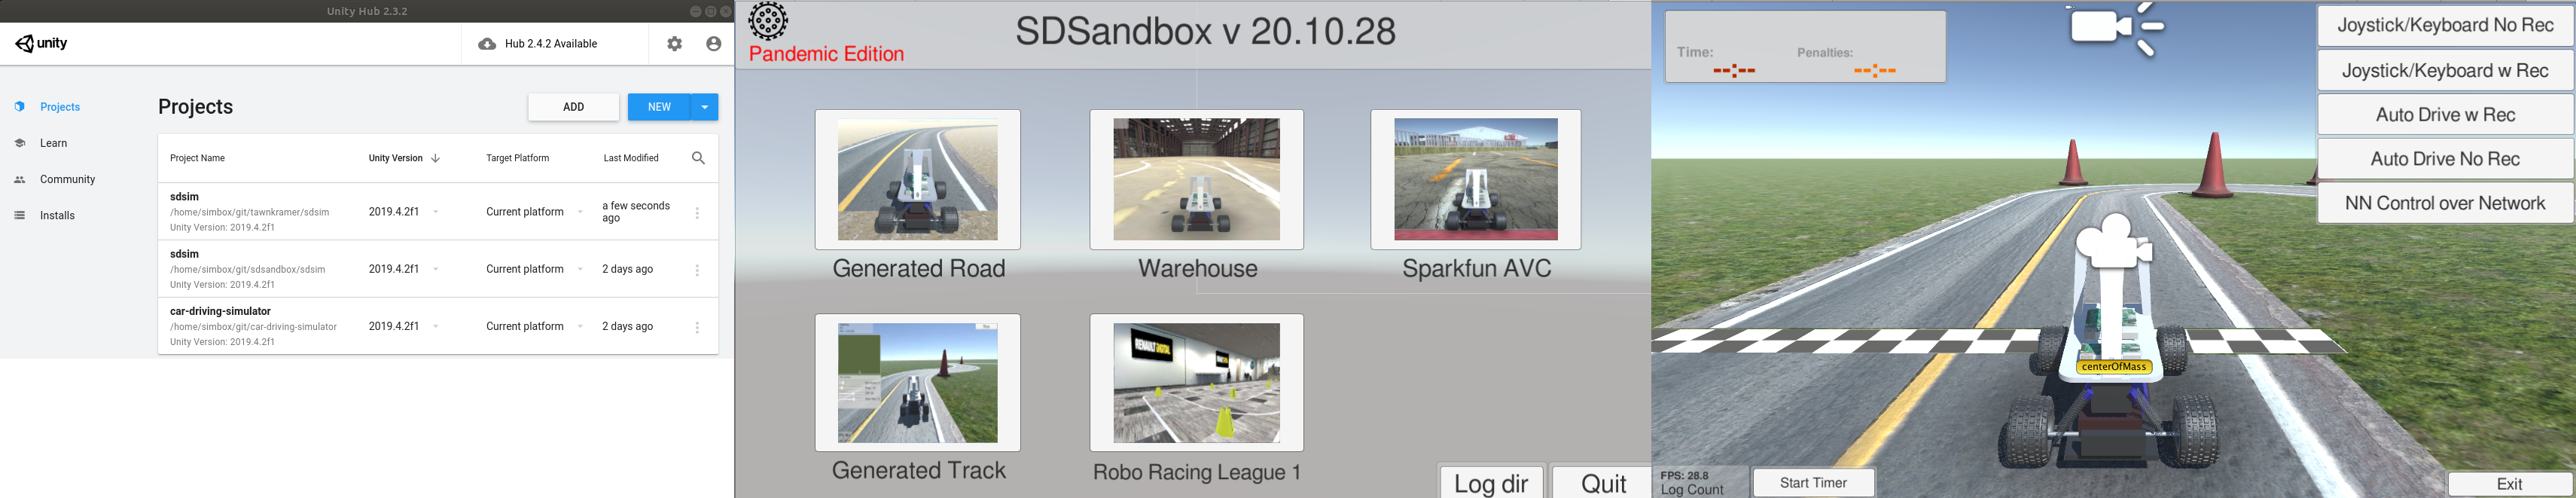
\includegraphics[scale=0.17]{Figures/UnityHubSDSandbox3in1.png}
 \caption{Left to right: Unity Hub, SDSandbox home screen and simulation ready to run}
 \label{fig:SDSandboxHome}
\end{figure}

\subsection{Installing the source code}
\label{installing-source-code}
The code is cloned from:
\begin{verbatim}
git clone https://github.com/dsikar/sdsandbox    
\end{verbatim}
This will download the source code to the sdsandbox directory.

\subsection{Running the Unity Hub application image}
\label{running-unity-hub}

\textit{Unity Hub} is downloaded to disk and started:
\begin{verbatim}
$ sudo ./UnityAppImage --no-sandbox
\end{verbatim}

\subsection{Adding the SDSanbox project to Unity Hub}

Once source code has been cloned, and Unity Hub is running, the project is added by clicking "ADD" and selecting directory sdsandbox/sdsim. The project will then appear as an list entry in Unity Hub and can be opened by clicking.

\subsection{Running the driving simulator}
\label{running-driving simulator}
Once the project is open, the "menu" scene is selected, and the play arrow button clicked. The simulator is ready to run.

\subsection{Recording one lap of training data}
\label{recording-one-lap}
Once the simulator is running, A "Log dir" log directory for storing data outputs is set, then "Generated Track" double-clicked, then "Auto Drive w Rec" option selected. This will set the simulator car going around the track. 
The control settings (displayed on main screen) are:
\begin{verbatim}
Max Speed: 1.772174
Prop: 49
Diff: 80
Steer Max: 25
\end{verbatim}
The are the maximum speed, the values Prop and Diff for updating steering angle and the maximum steering angle. Once a lap is completed, the Stop button is clicked, then the Play button is clicked to stop the simulator.  
Images in .jpg format and steering angles stored in .json files are created in sub-directory sdsim/log, and are ready to be moved to the "dataset" directory:
\begin{verbatim}
$ python prepare_data.py --out-path=../dataset/genTrack
\end{verbatim}
The previous command will move all images stored in the sim output directory to a date-labelled folder.

\section{Network monitoring and debugging with tcpflow}
\label{NetMonDebug}
tcpflow (\cite{garfinkel2013passive}) was used to monitor network traffic between car simulator and neural network prediction engine. Once the simulator is setup to run in neural network mode and before the predict\_client.py prediction engine starts, tcpflow is launched and set to listen on the loopback interface port 9091, and output network traffic packets to console:
\begin{verbatim}
$ sudo tcpflow -i lo -c port 9091
\end{verbatim}
The prediction script then runs and JSON, (\cite{pezoa2016foundations}) a lightweight data-interchange format, TCP encoded packets may be monitored and debugged. Simulator decoded packets are distinguished by \textit{telemetry} and prediction engine packets by \textit{control} msg\_types respectively, as shown in excerpt:
\begin{verbatim}
127. (...) {"msg_type":"telemetry",(...),"image":(...)
127. (...) {"msg_type": "control", "steering": "-0.09476048" (...)
\end{verbatim}
The packets carry the image sent from sim to prediction engine, and returned steering angle prediction.

\section{Generating Plots}

This section describe the tools used to generate plots.

\subsection{Steering angle comparison}

Plots were generated with Jupyter Notebook:
\begin{verbatim}
    src/utils/
\end{verbatim}

\section{Datasets}

A template directory structure was created such that downloaded data could be accessed in code with the same paths. The structure exists in the datasets repository and once cloned creates the template directory:
\begin{verbatim}
$ git clone https://github.com/dsikar/msc-data
$ tree -d msc-data/
msc-data/
 audi
 ford
 kitti
 mechanical-turk
 udacity
 unity
\end{verbatim}

\subsection{Ford AV Dataset}

The steering angles can be extracted from .bag files using ROS commands:
\begin{verbatim}
    # In one terminal, start ros engine
    $ roscore
    # In another terminal, inspect content of bag file
    $ time rosbag info Sample-Data.bag
    (...)
             /imu                 146939 msgs    : sensor_msgs/Imu             
    (...)
             /pose_ground_truth   146136 msgs    : geometry_msgs/PoseStamped   
             /pose_localized       16100 msgs    : geometry_msgs/PoseStamped   
             /pose_raw            146190 msgs    : geometry_msgs/PoseStamped   
(...)
    # And subscribe to topic of interest 
    $ rostopic echo /imu | tee sample_imu.yaml
    # In another terminal, playback bag file
    $ time rosbag play --immediate Sample-Data.bag --topics /imu
    # Sanity check, count number of acquisitions
    $ cat sample_imu.yaml | grep "orientation:" | wc -l
\end{verbatim}
The snippet above generates file imu.yaml, with all pose data generated by imu device. From this file we extract the steering angle, which is the z axis (yaw) of the orientation field (TODO check .yaml dialect). 
Images can be extracted from the same bag file with the Python 2.7 bag\_to\_images.py script:
\begin{verbatim}
    $ python2 bag_to_images.py Sample-Data.bag ~/git/msc-data/ford/sample/ros/ \
        /image_front_left
\end{verbatim}
Each image is an attribute in a dictionary, which also contains seconds (secs) and nano seconds (nsecs) attributes within the header attribute:
\begin{verbatim}
header: 
  seq: 213414
  stamp: 
    secs: 1501822147
    nsecs: 684951066
  frame_id: "camera_front_left"
height: 215
width: 414
encoding: "8UC3"
is_bigendian: 0
(...)
\end{verbatim}
Thus a timestamp can be obtained for each image extracted. This is done with script parse\_yaml\_time.py:
\begin{verbatim}
    
\end{verbatim}
While the steering angles are extracted 
The image can be matched with a steering angle by obtaining the timestamp of image, the full secs 

\subsection{Ford AV Dataset}
% Get details from https://avdata.ford.com/downloads/default.aspx
The Ford Autonomous Vehicle is a 
% angle from IMU
From % https://s23.q4cdn.com/258866874/files/doc_downloads/2020/03/2003.07969.pdf
 (\cite{Applanix}) is a professional-grade, compact,fully  integrated,  turnkey  position  and  orientation  system combining a differential GPS, an inertial measurement unit(IMU)  rated  with  1$^{\circ}$ of  drift  per  hour,  and  a  1024-count wheel encoder to measure the relative position, orientation,velocity,  angular  rate  and  acceleration  estimates  of  the vehicle. The Ford AV data set provides the 6-DOF pose (6DOF pose estimation of objects is the task of estimating the coordinates (X, Y,Z) and rotation angles (Yaw, Pitch and Roll) of an object with respect to a previously established reference coordinate system. (\cite{7005077} ) estimates obtained by integrating the (linear) acceleration and (angular) velocity.
% Note, Ford av authors discussion https://s23.q4cdn.com/258866874/files/doc_downloads/2020/03/2003.07969.pdf
% IEEE on 6DOF estimation from IMU discussion https://ieeexplore.ieee.org/document/7005077

% on converting GPS and IMU measurements to steering angles, see
% http://www.robesafe.uah.es/personal/roberto.arroyo/docs/Almazan13iv.pdf
% We might use a similar technique, time allowing

\subsection{Kitti}

The Kitti dataset TODO add provenance, add description
Data format, steering angle description obtained from oxts/dataformat.txt 
% cat 2011_09_26/2011_09_26_drive_0001_sync/oxts/dataformat.txt
\begin{verbatim}
yaw:   heading (rad),       0 = east,  positive = counter clockwise,\
    range: -pi   .. +pi
\end{verbatim}
Note, this may not be the steering angle - TBC. So additional work may be needed to obtain.
There are some pointers online, a simple approach seems to be:
% https://physics.stackexchange.com/questions/112301/calculating-the-rate-at-which-a-car-turns
This is also an interesting approach:
% http://docs.ros.org/en/kinetic/api/teb_local_planner_tutorials/html/cmd__vel__to__ackermann__drive_8py_source.html
With python code:
\begin{verbatim}
def convert_trans_rot_vel_to_steering_angle(v, omega, wheelbase):
  if omega == 0 or v == 0:
     return 0
  radius = v / omega
  return math.atan(wheelbase / radius)    
\end{verbatim}
Another possible method "Estimation of the Steering Angle Based on Extended Kalman-Filter"  
% http://gvpress.com/journals/IJMUE/vol11_no12/27.pdf
% equations 10 and 11


\section{Automold}
The rainy images were created with:  
\begin{verbatim}
github.com/dsikar/automold/RainyImagesDissertationPlot.ipynb
\end{verbatim}

\section{Development Environments}

Three development environments are planned to be used, a local environment to run the Unity3D SDSdanbox application, and two additional environments, the Intel Dev-Cloud (\cite{IntelDevCloud2020}) and City University's Camber server (\cite{Camber2019}).
% Further develop running jobs in these environments

\subsection{Intel DevCloud}

Intel provides a 200GB storage quota. Storage use can be checked with getquota command:
\begin{verbatim}
$ getquota
199.78 GB out of 200.00 GB (99.89%) used   
\end{verbatim}
Jobs are queued with qsub command:
\begin{verbatim}
    $ qsub -l nodes=1:gpu:ppn=2 ford_sample_download.sh -l walltime=23:59:59
\end{verbatim}
where the actual commands that run e.g. downloading data, training and testing networks are scripted in a batch file e.g. ford\_sample\_download.sh, train.sh.   
The queue can be checked with watch command:
\begin{verbatim}
    $ watch -n 1 qstat
\end{verbatim}
Jobs can run for a maximum of 24 hours, any job exceeding that execution time is terminated automatically. Jobs can be deleted from queue with qdel command.

\section{Unity}
Unity for Ubuntu is a single image file, that can be downloaded and run:
\begin{verbatim}
$ ./UnityHub.AppImage    
\end{verbatim}
This will start the Unity Hub app. A license must be installed by downloading a file, logging into Unity, uploading file then downloading a second license file. This is added to Unity Hub. The next step is to get an editor. Editors are available at:
\begin{verbatim}
https://unity3d.com/get-unity/download/archive    
\end{verbatim}
From archive pages, a link is obtained for desired editor (2019.3.0 is this case).
To load the editor, Unity Hub must be closed and the re-opened with the obtained link:
\begin{verbatim}
$ ./UnityHub.AppImage unityhub://2019.3.0f6/27ab2135bccf
\end{verbatim}
Source code for the simulator can then be cloned locally
\begin{verbatim}
git clone https://github.com/tawnkramer/sdsandbox.git    
\end{verbatim}
The project can then be added to Unity Hub by ADDing and navigating to sdsandbox/sdsim directory. It will then be listed on Unity Hub. Thereafter, Unity Hub can be started with
\begin{verbatim}
$ ./UnityHub.AppImage    
\end{verbatim}

\section{Tensorflow and Keras}
\label{methods:tensorflow-keras}
The versions used were 2.2.0 and 2.4.3 respectively. To ensure the same versions are installed in all development platforms, run:
\begin{verbatim}
$ pip install keras --user
$ pip install tensorflow --user
# to check versions
$ python3
>>> import keras
>>> keras.__version__
'2.4.3'
>>> import tensorflow
>>> tensorflow.__version__
'2.2.0'
\end{verbatim}
If the modules are already present in the environment, but a lower (earlier) version e.g.:
\begin{verbatim}
>>> tensorflow.__version__
'1.15.4'    
\end{verbatim}
it can be upgraded by running:
\begin{verbatim}
$ pip install --ignore-installed --upgrade tensorflow==2.2.0 --user
\end{verbatim}

\subsection{Recording one loop around a track}

To record the images and steering angles generated by going around a track once, on the terminal:
\begin{verbatim}
$ sudo ./UnityAppimage --no-sandbox
\end{verbatim}
Open the project in sdsim directory (commit ed0cc0b)

\subsection{Running simulator predictions}
\label{running-simulator-predictions}

To run predictions, and to monitor TCP traffic:
\begin{verbatim}
# Run unity from one terminal run:
$ sudo ./Unity.AppImage --no-sandbox
# To monitor TCP traffic, from another terminal run:
$ sudo tcpflow -i lo -c port 9091 > /tmp/tcpflow.log
# To run predictions, from another terminal run:
$ python predict_client.py \
--model=../trained_models/nvidia_baseline/20201120124421\_nvidia\_baseline.h5
\end{verbatim}

% there probably will not be enough time to use ROS at scale so parking this for now in appendix, might leave for future reference or remove
\section{ROS}
The Robot Operating System (\cite{quigley2009ros}) is middleware, that is, placed between the operating system an the application program. It helps manage complexity and distributed systems, such as a managing the process of recording several sensor outputs in a moving vehicle. The term "plumbing" is sometimes used, as parts of a distributed application are connection with "data pipes".  
ROS was used to store data from the FORD AV dataset.

% \section{Extracting steering angles with ROS}
Info on how to get a steering angle (YAW) using quaternions and the IMU data.

\section{Correspondence with supervisor}
\label{corr_with_super}
\subsection{Correspondence with Artur Garcez 1}
\begin{verbatim}
Garcez, Artur
Fri 14/02/2020 09:59
Hi Daniel,
See if you can find a data set which would offer you a systematic way of evaluating
how CNNs can be fooled by visual illusions caused by rain drops on the windscreen.
Artur
________________________________________
From: PG-Sikar, Daniel <Daniel.Sikar@city.ac.uk>
Sent: 14 February 2020 08:56
To: Garcez, Artur
Subject: MSC Data Science - Final year project

Hi Artur,

I am currently shopping around for a project. I have spoken to a couple of companies
but not sure data will be available in good time - ML applied to signal processing.

So I ask if you have any projects, ideally related to some kind of signal processing,
alternatively, anything related to computer vision which could potentially provide a
good hook for the self-driving car project we spoke (briefly) about?

Kind regards

Daniel - PT2    
\end{verbatim}

\subsection{Correspondence with Artur Garcez 2}
\label{met:corr_arthur_2}
\begin{verbatim}

Daniel,

Out of curiosity, is there any easy way of increasing glare from the sun in the 
simulator?

This would be a nice UK-specific example to give: a situation with light rain and glare 
possibly creating difficult illusions.

The big picture being there's not much hope training such models for billions of hours 
in California and transferring to London!

Best,
Artur    
\end{verbatim}

\section{Correspondence with authors}
\label{corr_with_authors}

\subsection{Correspondence with Urs Muller 1}
\label{urs_muller1}
Correspondence with \textbf{Urs Muller}, co-author of \cite{bojarski2016end}, with respect to network training settings.

\begin{verbatim}
From: Urs Muller <umuller@nvidia.com>Sent: 16 November 2020 19:30
To: PG-Sikar, Daniel <Daniel.Sikar@city.ac.uk>
Subject: Re: End to End Learning for Self-Driving Cars - Network Training Parameters

CAUTION: This email originated from outside of the organisation. 
Do not click links or open attachments unless you recognise the
sender and believe the content to be safe.

Hi Daniel,

We used the following settings (we haven't documented them in any publication):

loss function: MSE
optimizer: adadelta
learning rate: 1e-4 (but not really used in adadelta)
dropout: 0.25

Best regards,
Urs

From: PG-Sikar, Daniel <Daniel.Sikar@city.ac.uk>
Sent: Sunday, November 15, 2020 6:53To: Urs Muller <umuller@nvidia.com>
Subject: End to End Learning for Self-Driving Cars - Network Training Parameters
 
External email: Use caution opening links or attachments

Hi,

With respect to your network training, I am investigating the effect of noise 
(rainy images) on network performance, using your architecture as a baseline.

Would you be able to point me towards any documentation detailing loss function, 
learning rate, optimizer and layer droupout probabilities used when training 
your network?

Thanks in advance for any help and kind regards,

Daniel Sikar | MSc Data Science Candidate
School of Mathematics, Computer Science and Engineering
City University of London    
\end{verbatim}

\subsection{Correspondence with Urs Muller 2}
\label{urs_muller2}
\begin{verbatim}
Urs Muller <umuller@nvidia.com>
Tue 17/11/2020 11:47
CAUTION: This email originated from outside of the organisation. Do not click links or open attachments unless you recognise the sender and believe the content to be safe.

Hi Daniel,

Yes, correct. We cropped everything above the horizon. The lower edge of the crop is as low as possible before the road gets blocked by the hood of the car.

Best regards,
Urs
From: PG-Sikar, Daniel <Daniel.Sikar@city.ac.uk>
Sent: Tuesday, November 17, 2020 2:56
To: Urs Muller <umuller@nvidia.com>
Subject: Re: End to End Learning for Self-Driving Cars - Network Training Parameters
 
External email: Use caution opening links or attachments
Hi Urs,

Thanks for your reply. One more question with respect to the image size presented to your network - 66 pixel height by 200 width. Was this cropped from the size your camera sensors were generating? To keep only the road in the frame and omit anything above the horizon?

Kind regards,

Daniel    
\end{verbatim}

\subsection{Correspondence with Ankit Vora}
\label{ankit_vora}
Correspondence with \textbf{Ankit Vora}, co-author of \cite{agarwal2020ford}, with respect to extracting steering angles from rosbag files.

\begin{verbatim}
Vora, Ankit (A.) <avora3@ford.com>
Thu 05/11/2020 13:55
CAUTION: This email originated from outside of the organisation. 
Do not click links or open attachments unless you recognise the
sender and believe the content to be safe.

Hi Daniel,

The information you are looking for will be in the /pose_ground_truth message. 
That message represents the position and orientation of the vehicle.
You will have to convert quaternions to yaw, pitch, roll angles and
then use the yaw values.

Ankit
From: PG-Sikar, Daniel <Daniel.Sikar@city.ac.uk>
Sent: Wednesday, October 28, 2020 7:00 PM
To: Vora, Ankit (A.) <avora3@ford.com>
Subject: Ford AV Dataset - obtaining steering angles
 
Hi,
I am studying your AV datast and have extracted the /imu data from provided .bag files, 
I am trying to work out if the steering angle can be inferred from the data?
Your article states the dataset provides 6DOF pose estimation.
The extracted /imu topic looks like:

header:
  seq: 137596
  stamp:
    secs: 1501822140
    nsecs: 610330104
  frame_id: "imu"
orientation:
  x: 0.00133041249526
  y: 0.00486443211508
  z: 0.584795486661
  w: 0.811165091756
orientation_covariance: [0.0, 0.0, 0.0, 0.0, 0.0, 0.0, 0.0, 0.0, 0.0]
angular_velocity:
  x: -0.0018081133007
  y: -0.0105949952451
  z: -0.00118502619208
angular_velocity_covariance: [0.0, 0.0, 0.0, 0.0, 0.0, 0.0, 0.0, 0.0, 0.0]
linear_acceleration:
  x: -0.0136899789795
  y: 0.199539378285
  z: 0.305044800043
linear_acceleration_covariance: [0.0, 0.0, 0.0, 0.0, 0.0, 0.0, 0.0, 0.0, 0.0]

I guess I am interested in the yaw, which would be the value z, but
having looking at the pattern it does not look like an angle that
could be associated to steering, positive and negative values close
to zero.

Could you help me identify the steering angle, or if it is not
present suggest any approaches to extract it from the data?

Anyway help would be greatly appreciated.

Daniel Sikar
Daniel Sikar | MSc Data Science Candidate
School of Mathematics, Computer Science and Engineering
City University of London   
\end{verbatim}

\subsection{Correspondence with Maxime Ellerbach}
\label{corr:ellerbach}
On the majority of the Donkey Race community using behavioural cloning for self-driving CNN training.

Maxime Ellerbach is the main maintainer of the SDSandbox project. 

\begin{verbatim}
Maxime Ellerbach
	
14 Nov 2020, 14:44 (4 days ago)
	
Oh, I think the drive menu is quite old, it was added before May update,
at this time Tawn was still doing the changes.
Now I'm the main maintainer of the project, for the moment I'm mainly
doing some backend changes to make the track creation process easier.

For the training part, most of us use behavioral cloning !
But they are mostly using the donkeycar framework, on my side I don't
use any framework and it performs great.
I would be happy if you could join us in a next virtual race !

Cheers,
Maxime

-----Message d'origine-----
De : Daniel Sikar <dsikar@gmail.com>
Envoyé : samedi 14 novembre 2020 15:25

À : Maxime Ellerbach <maxime@ellerbach.net>
Objet : Re: SDSandbox output image size

Thanks, that is super helpful. What really helped me was the drive menu being added to
the Generated Track.
I have not checked closely the commit history (I have been following SDSandbox since
February) but given you have been the most active user I take it was from you.
I did add some data augmentation to training that I thought might be helpful for others
doing behavioural cloning, but understand that most (or all) of you in the virtual race
league are using reinforcement learning models, making more use out of the Dokey-Gym
environment than I am. Anyway, I hope to get to RL before long and to join the league!
Daniel

\end{verbatim}

%%%%%%%%%%%%%%%%%%%%%%%%%%%%%%%%%%%%%%%%%%%%%%%%%%%%%%%%%%%%%%%%%%%%%%%%%%%%%
% Mechanical Turk
%%%%%%%%%%%%%%%%%%%%%%%%%%%%%%%%%%%%%%%%%%%%%%%%%%%%%%%%%%%%%%%%%%%%%%%%%%%%%

\section{Locating rainy sections with Mechanical Turk}
For Mechanical Turk, the data that looked most promising was Ford V2 Log 1 and V3 Log 1, both described as "freeway, overpass, bridge, cloudy". We drew 50 images uniformly from each log and added 5 images with rain that were expected to be labelled as such. The 105 images were then added to a SageMaker Ground Truth job. The platform works as a wrapper around Mechanical Turk as it facilitates the creation of user interfaces (Figure \ref{fig:MechTurkCreateJob})
% rainy files created with automold/RainyImagesDissertationPlot.ipynb
\begin{figure}[h!]
\centering
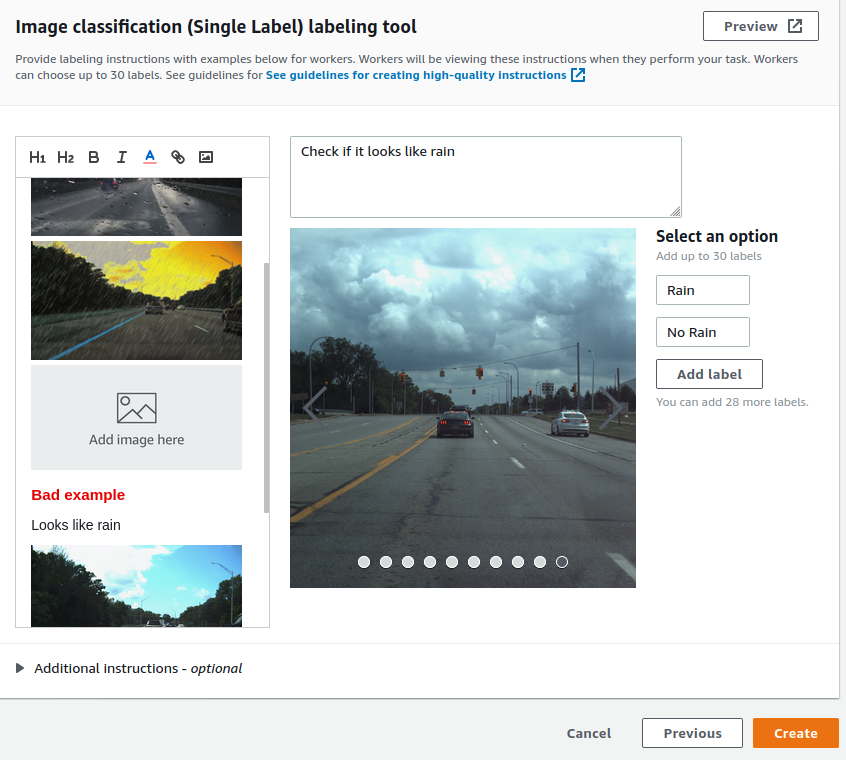
\includegraphics[width=10cm]{Figures/MechTurkCreateJob.png}
\caption{The SageMaker Ground Truth user interface template with two labels ("Rain", "No Rain"), the image to be labeled and examples of correct and incorrect classifications.}
\label{fig:MechTurkCreateJob}
\end{figure}
Labeling tasks are classified as low, medium and high complexity. The prices range from \$0.012 for a low complexity task, with a 5 second estimate to complete, to \$1.20 for a high complexity task with a 3.5 minute estimate to complete.
The task can be configured with an output for time taken by a worker on a single task, the lowest time interval being one minute.
There is also an option to assign more than one worker per dataset object, on account that it can help increase the accuracy of the data labels.
The task was created with the most basic options of one worker, a \$0.012 price per task, a one minute timeout and remained live for 12 hours. 
The images were labelled by Mechanical Turk workers and results made available in a json encoded file (datasets/mechanical-turk/2020-11-21\_22 45 37.json) showing no images had been labeled as "Rain". The assumption then being there are no sections containing rain in the dataset. The Automold library added rain images were also labeled as "No Rain". Figure \ref{fig:MechTurkLabeledImages}
\begin{figure}[h!]
\centering
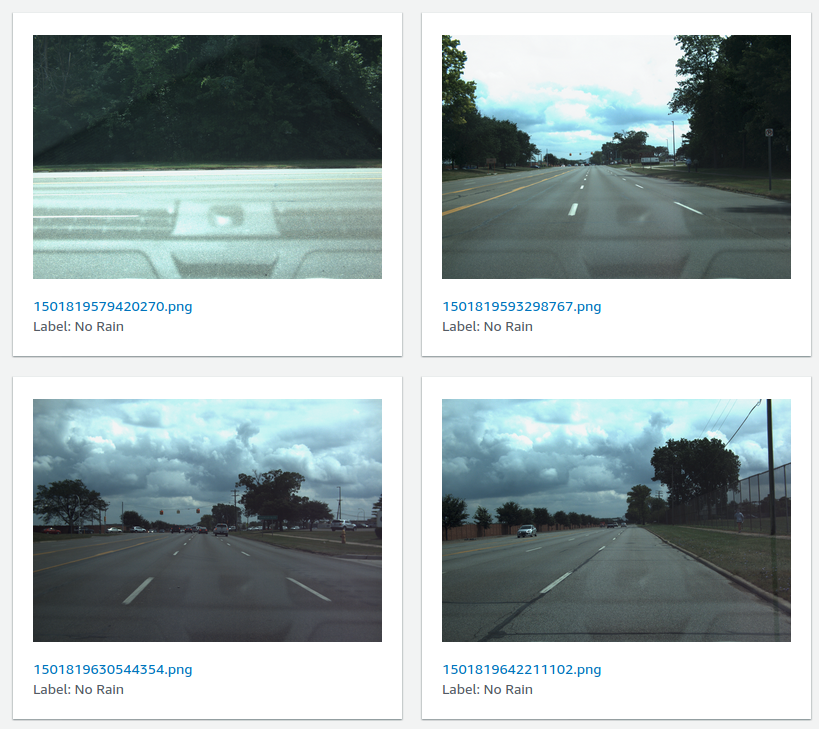
\includegraphics[width=10cm]{Figures/MechTurkLabeledImages.png}
\caption{The SageMaker Ground Truth labeled images detail on Labeling Job Summary page}
\label{fig:MechTurkLabeledImages}
\end{figure}
%\chapter{Network architectures} % Main appendix title

\label{AppendixB} % For referencing this appendix elsewhere, use \ref{AppendixX}
%%%%%%%%%%%%%%%%%%%%%%%%%%%%%%%%%%%%%%%%%%%%%%%%%
% NVIDIA_BASELINE
%%%%%%%%%%%%%%%%%%%%%%%%%%%%%%%%%%%%%%%%%%%%%%%%%
\section{NVIDIA baseline architecture}
\label{NVIDIA_baseline}
\label{arc:nvidia_baseline}

This is the starting point after the work of \cite{bojarski2016end}

\begin{verbatim}
>>> import models
>>> mymodel = models.nvidia_baseline(1)
>>> models.show_model_summary(mymodel)
Model: "model"
_________________________________________________________________
Layer (type)                 Output Shape              Param #   
=================================================================
img_in (InputLayer)          [(None, 66, 200, 3)]      0         
_________________________________________________________________
lambda (Lambda)              (None, 66, 200, 3)        0         
_________________________________________________________________
conv2d_1 (Conv2D)            (None, 31, 98, 24)        1824      
_________________________________________________________________
dropout (Dropout)            (None, 31, 98, 24)        0         
_________________________________________________________________
conv2d_2 (Conv2D)            (None, 14, 47, 36)        21636     
_________________________________________________________________
dropout_1 (Dropout)          (None, 14, 47, 36)        0         
_________________________________________________________________
conv2d_3 (Conv2D)            (None, 5, 22, 48)         43248     
_________________________________________________________________
dropout_2 (Dropout)          (None, 5, 22, 48)         0         
_________________________________________________________________
conv2d_4 (Conv2D)            (None, 3, 20, 64)         27712     
_________________________________________________________________
dropout_3 (Dropout)          (None, 3, 20, 64)         0         
_________________________________________________________________
conv2d_5 (Conv2D)            (None, 1, 18, 64)         36928     
_________________________________________________________________
dropout_4 (Dropout)          (None, 1, 18, 64)         0         
_________________________________________________________________
flattened (Flatten)          (None, 1152)              0         
_________________________________________________________________
dense_1 (Dense)              (None, 1164)              1342092   
_________________________________________________________________
dropout_5 (Dropout)          (None, 1164)              0         
_________________________________________________________________
dense_2 (Dense)              (None, 100)               116500    
_________________________________________________________________
dropout_6 (Dropout)          (None, 100)               0         
_________________________________________________________________
dense_3 (Dense)              (None, 50)                5050      
_________________________________________________________________
dropout_7 (Dropout)          (None, 50)                0         
_________________________________________________________________
dense_4 (Dense)              (None, 10)                510       
_________________________________________________________________
dropout_8 (Dropout)          (None, 10)                0         
_________________________________________________________________
steering (Dense)             (None, 1)                 11        
=================================================================
Total params: 1,595,511
Trainable params: 1,595,511
Non-trainable params: 0
_________________________________________________________________
[(None, 66, 200, 3)]
(None, 66, 200, 3)
(None, 31, 98, 24)
(None, 31, 98, 24)
(None, 14, 47, 36)
(None, 14, 47, 36)
(None, 5, 22, 48)
(None, 5, 22, 48)
(None, 3, 20, 64)
(None, 3, 20, 64)
(None, 1, 18, 64)
(None, 1, 18, 64)
(None, 1152)
(None, 1164)
(None, 1164)
(None, 100)
(None, 100)
(None, 50)
(None, 50)
(None, 10)
(None, 10)
(None, 1)
\end{verbatim}

%%%%%%%%%%%%%%%%%%%%%%%%%%%%%%%%%%%%%%%%%%%%%%%%%
% NVIDIA1 - Commit 55cb00b
%%%%%%%%%%%%%%%%%%%%%%%%%%%%%%%%%%%%%%%%%%%%%%%%%
\section{NVIDIA1 architecture}
\label{arc:nvidia1}
The network architecture is as shown, with a total of 817,028 trainable parameters. The design is exactly as used by \cite{SDSandboxSim}.
\begin{verbatim}
>>> import models
>>> mymodel = models.nvidia_model1(2)
>>> models.show_model_summary(mymodel)
Model: "model_3"
_________________________________________________________________
Layer (type)                 Output Shape              Param #   
=================================================================
img_in (InputLayer)          [(None, 120, 160, 3)]     0         
_________________________________________________________________
lambda_3 (Lambda)            (None, 120, 160, 3)       0         
_________________________________________________________________
conv2d_1 (Conv2D)            (None, 58, 78, 24)        1824      
_________________________________________________________________
dropout_15 (Dropout)         (None, 58, 78, 24)        0         
_________________________________________________________________
conv2d_2 (Conv2D)            (None, 27, 37, 32)        19232     
_________________________________________________________________
dropout_16 (Dropout)         (None, 27, 37, 32)        0         
_________________________________________________________________
conv2d_3 (Conv2D)            (None, 12, 17, 64)        51264     
_________________________________________________________________
dropout_17 (Dropout)         (None, 12, 17, 64)        0         
_________________________________________________________________
conv2d_4 (Conv2D)            (None, 10, 15, 64)        36928     
_________________________________________________________________
dropout_18 (Dropout)         (None, 10, 15, 64)        0         
_________________________________________________________________
conv2d_5 (Conv2D)            (None, 8, 13, 64)         36928     
_________________________________________________________________
dropout_19 (Dropout)         (None, 8, 13, 64)         0         
_________________________________________________________________
flattened (Flatten)          (None, 6656)              0         
_________________________________________________________________
dense_6 (Dense)              (None, 100)               665700    
_________________________________________________________________
dense_7 (Dense)              (None, 50)                5050      
_________________________________________________________________
steering_throttle (Dense)    (None, 2)                 102       
=================================================================
Total params: 817,028
Trainable params: 817,028
Non-trainable params: 0
_________________________________________________________________
[(None, 120, 160, 3)]
(None, 120, 160, 3)
(None, 58, 78, 24)
(None, 58, 78, 24)
(None, 27, 37, 32)
(None, 27, 37, 32)
(None, 12, 17, 64)
(None, 12, 17, 64)
(None, 10, 15, 64)
(None, 10, 15, 64)
(None, 8, 13, 64)
(None, 8, 13, 64)
(None, 6656)
(None, 100)
(None, 50)
(None, 2)    
\end{verbatim}

%%%%%%%%%%%%%%%%%%%%%%%%%%%%%%%%%%%%%%%%%%%%%%%%%
% NVIDIA2 - Commit df953d2
%%%%%%%%%%%%%%%%%%%%%%%%%%%%%%%%%%%%%%%%%%%%%%%%%
\section{NVIDIA2 Architecture}
\label{arc:nvidia2}
\begin{verbatim}
>>> import models
>>> mymodel = models.nvidia_model2(2)
>>> models.show_model_summary(mymodel)
Model: "model"
_________________________________________________________________
Layer (type)                 Output Shape              Param #   
=================================================================
img_in (InputLayer)          [(None, 66, 200, 3)]      0         
_________________________________________________________________
lambda (Lambda)              (None, 66, 200, 3)        0         
_________________________________________________________________
conv2d_1 (Conv2D)            (None, 31, 98, 24)        1824      
_________________________________________________________________
dropout (Dropout)            (None, 31, 98, 24)        0         
_________________________________________________________________
conv2d_2 (Conv2D)            (None, 14, 47, 32)        19232     
_________________________________________________________________
dropout_1 (Dropout)          (None, 14, 47, 32)        0         
_________________________________________________________________
conv2d_3 (Conv2D)            (None, 5, 22, 48)         38448     
_________________________________________________________________
dropout_2 (Dropout)          (None, 5, 22, 48)         0         
_________________________________________________________________
conv2d_4 (Conv2D)            (None, 3, 20, 64)         27712     
_________________________________________________________________
dropout_3 (Dropout)          (None, 3, 20, 64)         0         
_________________________________________________________________
conv2d_5 (Conv2D)            (None, 1, 18, 64)         36928     
_________________________________________________________________
dropout_4 (Dropout)          (None, 1, 18, 64)         0         
_________________________________________________________________
flattened (Flatten)          (None, 1152)              0         
_________________________________________________________________
dense (Dense)                (None, 100)               115300    
_________________________________________________________________
dense_1 (Dense)              (None, 50)                5050      
_________________________________________________________________
dense_2 (Dense)              (None, 10)                510       
_________________________________________________________________
steering_throttle (Dense)    (None, 2)                 22        
=================================================================
Total params: 245,026    
Trainable params: 245,026
Non-trainable params: 0
_________________________________________________________________
[(None, 66, 200, 3)]
(None, 66, 200, 3)
(None, 31, 98, 24)
(None, 31, 98, 24)
(None, 14, 47, 32)
(None, 14, 47, 32)
(None, 5, 22, 48)
(None, 5, 22, 48)
(None, 3, 20, 64)
(None, 3, 20, 64)
(None, 1, 18, 64)
(None, 1, 18, 64)
(None, 1152)
(None, 100)
(None, 50)
(None, 10)
(None, 2)

\end{verbatim}


%%%%%%%%%%%%%%%%%%%%%%%%%%%%%%%%%%%%%%%%%%%%%%%%%
% NVIDIA2
%%%%%%%%%%%%%%%%%%%%%%%%%%%%%%%%%%%%%%%%%%%%%%%%%
\section{Alexnet}
Adapted to achieve same geometry - NB Input size (described as 224x224) is suggested to  be 227x227 \cite{CS231n}. 
Though changing kernel size to 8x8 also generates a 55x55 feature map in the first convolutional layer.

\begin{verbatim}
models.show_model_summary(model)
Model: "model"
_________________________________________________________________
Layer (type)                 Output Shape              Param #   
=================================================================
img_in (InputLayer)          [(None, 224, 200, 3)]     0         
_________________________________________________________________
lambda (Lambda)              (None, 224, 200, 3)       0         
_________________________________________________________________
conv2d_1 (Conv2D)            (None, 55, 49, 48)        9264      
_________________________________________________________________
maxpool2d_1 (MaxPooling2D)   (None, 55, 49, 48)        0         
_________________________________________________________________
conv2d_2 (Conv2D)            (None, 27, 24, 128)       55424     
_________________________________________________________________
maxpool2d_2 (MaxPooling2D)   (None, 27, 24, 128)       0         
_________________________________________________________________
conv2d_3 (Conv2D)            (None, 13, 11, 192)       221376    
_________________________________________________________________
conv2d_4 (Conv2D)            (None, 13, 11, 192)       331968    
_________________________________________________________________
conv2d_5 (Conv2D)            (None, 13, 11, 128)       221312    
_________________________________________________________________
maxpool2d_3 (MaxPooling2D)   (None, 13, 11, 128)       0         
_________________________________________________________________
dropout (Dropout)            (None, 13, 11, 128)       0         
_________________________________________________________________
flattened (Flatten)          (None, 18304)             0         
_________________________________________________________________
Dense_1 (Dense)              (None, 2048)              37488640  
_________________________________________________________________
Dense_2 (Dense)              (None, 50)                102450    
_________________________________________________________________
dense (Dense)                (None, 10)                510       
_________________________________________________________________
steering_throttle (Dense)    (None, 2)                 22        
=================================================================
Total params: 38,430,966
Trainable params: 38,430,966
Non-trainable params: 0
_________________________________________________________________
[(None, 224, 200, 3)]
(None, 224, 200, 3)
(None, 55, 49, 48)
(None, 55, 49, 48)
(None, 27, 24, 128)
(None, 27, 24, 128)
(None, 13, 11, 192)
(None, 13, 11, 192)
(None, 13, 11, 128)
(None, 13, 11, 128)
(None, 13, 11, 128)
(None, 18304)
(None, 2048)
(None, 50)
(None, 10)
(None, 2)
\end{verbatim}

\section{Training and testing networks}
A network is trained by running the script:
\begin{verbatim}
$ python --model=nvidia1
    --outdir=../trained_models
    --epochs=1
    --inputs=../dataset/unity/roboleague/log/*.jpg
    --aug=false
    --crop=false    
\end{verbatim}
This will generate a model, saved in the .h5 format, a python dictionary object with training and testing accuracy and loss values, and an accuracy and loss plot with information additional labels to help identify the trained model. Finally, a log file is saved to disk containing model name, training time and last recorded loss and accuracy values for training and testing datasets.

run experiment on vanilla code (no augmentation)
Record cash crash and deviation from actual to predicted steering angles.


%\chapter{Deliverables} % Main appendix title

\label{AppendixC-deliverables} % For referencing this appendix elsewhere, use \ref{AppendixX}

We have identified 92 deliverables for our practical research. Table \ref{Deliverables-Datasets} refers to datasets that will be used to train our models. Table \ref{Deliverables-Simulators} refers to the simulator tracks used to test models. Table \ref{Deliverables-Models} refers to the models (i.e. network architectures) to be trained with our datasets and tested on our simulator tracks, finally tables \ref{Deliverables-NVIDIA} through to \ref{Deliverables-ResNet} refer to training tasks performed with a permutation of models and datasets, and metrics obtained by testing each model on each simulator track.

%% DELIVERABLES - DATA

\begin{table}[]
\begin{center}
\begin{tabular}{|l|l|l|l|}
\hline
\multicolumn{4}{|c|}{Deliverables - Datasets} \\ \hline

%ID Task Deliverable Description
%1   Download  D1  Udacity real world dataset
%2   Generate    D2  Udacity simulator data
%3   Combine D3  Udacity real and simulator data
%4   Mechanical Turk dry/rainy Ford dataset

ID & Task &  Deliverable & Description \\ \hline\hline
1 & Download & D1 &  Udacity real world dataset  \\ \hline
2 & Generate & D2 &  Unity3D simulator data  \\ \hline
3 & Combine & D3 &  Udacity real and Unity3D simulator data  \\ \hline
4 & Gather & D4 &  Mechanical Turk dry/rainy Ford dataset  \\ \hline

\end{tabular}
\end{center}
\caption{Datasets used to train models}
\label{Deliverables-Datasets}
\end{table}

%% DELIVERABLES - SIMULATOR TRACKS

\begin{table}[]
\begin{center}
\begin{tabular}{|l|l|l|l|}
\hline
\multicolumn{4}{|c|}{Deliverables - Simulator testing tracks} \\ \hline

%ID  Task    Deliverable Description
%5   Build   S1  Unity simulator sunny/dry   
%6   Build   S2  Unity simulator added rain/reflections 1   
%7   Build   S3  Unity simulator added rain/reflections 2   

ID & Task &  Deliverable & Description \\ \hline\hline
5 & Build & S1 &  Unity simulator sunny/dry  \\ \hline
6 & Build & S2 &  Unity simulator added rain/reflections 1 \\ \hline
7 & Build & S3 &  Unity simulator added rain/reflections 2 \\ \hline

\end{tabular}
\end{center}
\caption{Simulator tracks to test models}
\label{Deliverables-Simulators}
\end{table}

%% DELIVERABLES - MODELS

\begin{table}[]
\begin{center}
\begin{tabular}{|l|l|l|l|}
\hline
\multicolumn{4}{|c|}{Deliverables - Models} \\ \hline

%ID  Task    Deliverable Description
%8   Build   N1  NVIDIA end-to-end architecture
%9   Build   N2  AlexNet
%10  Build   N3  VGGNet
%11  Build   N4  InceptionNet
%12  Build   N5  ResNet   

ID & Task &  Deliverable & Description \\ \hline\hline
8 & Build & N1 &  NVIDIA end-to-end architecture  \\ \hline
9 & Build & N2 &  AlexNet \\ \hline
10 & Build & N3 &  VGGNet \\ \hline
11 & Build & N4 &  InceptionNet \\ \hline
12 & Build & N5 &  ResNet \\ \hline

\end{tabular}
\end{center}
\caption{Models to be trained and tested}
\label{Deliverables-Models}
\end{table}

%% DELIVERABLES - MODELS AND METRICS

%%%%%%%%%%%%%%%%%%%%%%%%

% NVIDIA

\begin{table}[]
\begin{center}
\begin{tabular}{|l|l|l|l|l|l|}
\hline
\multicolumn{6}{|c|}{Deliverables - NVIDIA} \\ \hline

ID & Task &  Network/Model & Data/Sim & Deliverable & Description \\ \hline\hline
13 & Train & N1 & D1 & N1M1 & Model \\ \hline
14 & Test & N1M1 & S1 & N1R1 & Metric \\ \hline
15 & Test & N1M1 & S2 & N1R2 & Metric \\ \hline
16 & Test & N1M1 & S3 & N1R3 & Metric \\ \hline\hline

17 & Train & N1 & D2 & N1M2 & Model \\ \hline
18 & Test & N1M2 & S1 & N1R3 & Metric \\ \hline
19 & Test & N1M2 & S2 & N1R4 & Metric \\ \hline
20 & Test & N1M2 & S3 & N1R5 & Metric \\ \hline\hline

21 & Train & N1 & D3 & N1M3 & Model \\ \hline
22 & Test & N1M3 & S1 & N1R7 & Metric \\ \hline
23 & Test & N1M3 & S2 & N1R8 & Metric \\ \hline
24 & Test & N1M3 & S3 & N1R9 & Metric \\ \hline\hline

25 & Train & N1 & D4 & N1M4 & Model \\ \hline
26 & Test & N1M4 & S1 & N1R10 & Metric \\ \hline
27 & Test & N1M4 & S2 & N1R11 & Metric \\ \hline
28 & Test & N1M4 & S3 & N1R12 & Metric \\ \hline 

\end{tabular}
\end{center}
\caption{NVIDIA model and metric deliverables}
\label{Deliverables-NVIDIA}
\end{table}

%%%%%%%%%%%%%%%%%%%%%%%%

% AlexNet

\begin{table}[]
\begin{center}
\begin{tabular}{|l|l|l|l|l|l|}
\hline
\multicolumn{6}{|c|}{Deliverables - AlexNet} \\ \hline

ID & Task &  Network/Model & Data/Sim & Deliverable & Description \\ \hline\hline
29 & Train & N2 & D1 & N2M1 & Model \\ \hline
30 & Test & N2M1 & S1 & N2R1 & Metric \\ \hline
31 & Test & N2M1 & S2 & N2R2 & Metric \\ \hline
32 & Test & N2M1 & S3 & N2R3 & Metric \\ \hline\hline

33 & Train & N2 & D2 & N2M2 & Model \\ \hline
34 & Test & N2M2 & S1 & N2R3 & Metric \\ \hline
35 & Test & N2M2 & S2 & N2R4 & Metric \\ \hline
36 & Test & N2M2 & S3 & N2R5 & Metric \\ \hline\hline

37 & Train & N2 & D3 & N2M3 & Model \\ \hline
38 & Test & N2M3 & S1 & N2R7 & Metric \\ \hline
39 & Test & N2M3 & S2 & N2R8 & Metric \\ \hline
40 & Test & N2M3 & S3 & N2R9 & Metric \\ \hline\hline

41 & Train & N2 & D4 & N2M4 & Model \\ \hline
42 & Test & N2M4 & S1 & N2R10 & Metric \\ \hline
43 & Test & N2M4 & S2 & N2R11 & Metric \\ \hline
44 & Test & N2M4 & S3 & N2R12 & Metric \\ \hline 

\end{tabular}
\end{center}
\caption{AlexNet model and metric deliverables}
\label{Deliverables-AlexNet}
\end{table}

%%%%%%%%%%%%%%%%%%%%%%%%

% VGGNet

\begin{table}[]
\begin{center}
\begin{tabular}{|l|l|l|l|l|l|}
\hline
\multicolumn{6}{|c|}{Deliverables - VGGNet} \\ \hline

ID & Task &  Network/Model & Data/Sim & Deliverable & Description \\ \hline\hline
45 & Train & N3 & D1 & N3M1 & Model \\ \hline
46 & Test & N3M1 & S1 & N3R1 & Metric \\ \hline
47 & Test & N3M1 & S2 & N3R2 & Metric \\ \hline
48 & Test & N3M1 & S3 & N3R3 & Metric \\ \hline\hline

49 & Train & N3 & D2 & N3M2 & Model \\ \hline
50 & Test & N3M2 & S1 & N3R3 & Metric \\ \hline
51 & Test & N3M2 & S2 & N3R4 & Metric \\ \hline
52 & Test & N3M2 & S3 & N3R5 & Metric \\ \hline\hline

53 & Train & N3 & D3 & N3M3 & Model \\ \hline
54 & Test & N3M3 & S1 & N3R7 & Metric \\ \hline
55 & Test & N3M3 & S2 & N3R8 & Metric \\ \hline
56 & Test & N3M3 & S3 & N3R9 & Metric \\ \hline\hline

57 & Train & N3 & D4 & N3M4 & Model \\ \hline
58 & Test & N3M4 & S1 & N3R10 & Metric \\ \hline
59 & Test & N3M4 & S2 & N3R11 & Metric \\ \hline
60 & Test & N3M4 & S3 & N3R12 & Metric \\ \hline 

\end{tabular}
\end{center}
\caption{VGGNet model and metric deliverables}
\label{Deliverables-VGGNet}
\end{table}

%%%%%%%%%%%%%%%%%%%%%%%%

% InceptionNet

\begin{table}[]
\begin{center}
\begin{tabular}{|l|l|l|l|l|l|}
\hline
\multicolumn{6}{|c|}{Deliverables - InceptionNet} \\ \hline

ID & Task &  Network/Model & Data/Sim & Deliverable & Description \\ \hline\hline
61 & Train & N4 & D1 & N4M1 & Model \\ \hline
62 & Test & N4M1 & S1 & N4R1 & Metric \\ \hline
63 & Test & N4M1 & S2 & N4R2 & Metric \\ \hline
64 & Test & N4M1 & S3 & N4R3 & Metric \\ \hline\hline

65 & Train & N4 & D2 & N4M2 & Model \\ \hline
66 & Test & N4M2 & S1 & N4R3 & Metric \\ \hline
67 & Test & N4M2 & S2 & N4R4 & Metric \\ \hline
68 & Test & N4M2 & S3 & N4R5 & Metric \\ \hline\hline

69 & Train & N4 & D3 & N4M3 & Model \\ \hline
70 & Test & N4M3 & S1 & N4R7 & Metric \\ \hline
71 & Test & N4M3 & S2 & N4R8 & Metric \\ \hline
72 & Test & N4M3 & S3 & N4R9 & Metric \\ \hline\hline

73 & Train & N4 & D4 & N4M4 & Model \\ \hline
74 & Test & N4M4 & S1 & N4R10 & Metric \\ \hline
75 & Test & N4M4 & S2 & N4R11 & Metric \\ \hline
76 & Test & N4M4 & S3 & N4R12 & Metric \\ \hline 

\end{tabular}
\end{center}
\caption{InceptionNet model and metric deliverables}
\label{Deliverables-InceptionNet}
\end{table}

%%%%%%%%%%%%%%%%%%%%%%%%

% ResNet

\begin{table}[]
\begin{center}
\begin{tabular}{|l|l|l|l|l|l|}
\hline
\multicolumn{6}{|c|}{Deliverables - ResNet} \\ \hline

ID & Task &  Network/Model & Data/Sim & Deliverable & Description \\ \hline\hline
77 & Train & N5 & D1 & N5M1 & Model \\ \hline
78 & Test & N5M1 & S1 & N5R1 & Metric \\ \hline
79 & Test & N5M1 & S2 & N5R2 & Metric \\ \hline
80 & Test & N5M1 & S3 & N5R3 & Metric \\ \hline\hline

81 & Train & N5 & D2 & N5M2 & Model \\ \hline
82 & Test & N5M2 & S1 & N5R3 & Metric \\ \hline
83 & Test & N5M2 & S2 & N5R4 & Metric \\ \hline
84 & Test & N5M2 & S3 & N5R5 & Metric \\ \hline\hline

85 & Train & N5 & D3 & N5M3 & Model \\ \hline
86 & Test & N5M3 & S1 & N5R7 & Metric \\ \hline
87 & Test & N5M3 & S2 & N5R8 & Metric \\ \hline
88 & Test & N5M3 & S3 & N5R9 & Metric \\ \hline\hline

89 & Train & N5 & D4 & N5M4 & Model \\ \hline
90 & Test & N5M4 & S1 & N5R10 & Metric \\ \hline
91 & Test & N5M4 & S2 & N5R11 & Metric \\ \hline
92 & Test & N5M4 & S3 & N5R12 & Metric \\ \hline 

\end{tabular}
\end{center}
\caption{ResNet model and metric deliverables}
\label{Deliverables-ResNet}
\end{table}
% \chapter{Results} % Main appendix title

\label{AppendixD} % For referencing this appendix elsewhere, use \ref{AppendixX}

\section{Ford AV Dataset steering angles}

\subsection{Ford AV Dataset}

The steering angles can be extracted from .bag files using ROS commands:
\begin{verbatim}
    # In one terminal, start ros engine
    $ roscore
    # In another terminal, inspect content of bag file
    $ time rosbag info Sample-Data.bag
    (...)
             /imu                 146939 msgs    : sensor_msgs/Imu             
    (...)
             /pose_ground_truth   146136 msgs    : geometry_msgs/PoseStamped   
             /pose_localized       16100 msgs    : geometry_msgs/PoseStamped   
             /pose_raw            146190 msgs    : geometry_msgs/PoseStamped   
(...)
    # And subscribe to topic of interest 
    $ rostopic echo /imu | tee sample_imu.yaml
    # In another terminal, playback bag file
    $ time rosbag play --immediate Sample-Data.bag --topics /imu
    # Sanity check, count number of acquisitions
    $ cat sample_imu.yaml | grep "orientation:" | wc -l
\end{verbatim}
The snippet above generates file imu.yaml, with all pose data generated by imu device. From this file we extract the steering angle, which is the z axis (yaw) of the orientation field (TODO check .yaml dialect). 
Images can be extracted from the same bag file with the Python 2.7 bag\_to\_images.py script:
\begin{verbatim}
    $ python2 bag_to_images.py Sample-Data.bag ~/git/msc-data/ford/sample/ros/ \
        /image_front_left
\end{verbatim}
Each image is an attribute in a dictionary, which also contains seconds (secs) and nano seconds (nsecs) attributes within the header attribute:
\begin{verbatim}
header: 
  seq: 213414
  stamp: 
    secs: 1501822147
    nsecs: 684951066
  frame_id: "camera_front_left"
height: 215
width: 414
encoding: "8UC3"
is_bigendian: 0
(...)
\end{verbatim}
Thus a timestamp can be obtained for each image extracted. This is done with script parse\_yaml\_time.py:
\begin{verbatim}
    
\end{verbatim}
While the steering angles are extracted 
The image can be matched with a steering angle by obtaining the timestamp of image, the full secs 

\section{Audi}

The  Audi Autonomous Driving Dataset (A2D2)
authors (\cite{geyer2020a2d2}) are motivated by the fact that research in machine learning, mobile robotics and autonomous driving is accelerated by the availability of high quality annotated data. This statement can be verified by the advances in image classification with deep neural networks since \cite{IMAGENET} became available.  
The A2D2 data was acquired with a human-driven Audi Q7 e-tron equipped with six cameras (front left, front center, front right, back left, back center, back right) and five LiDAR sensors. The authors claim this resulted in  360$^{\circ}$ camera and LiDAR coverage. Additionally, several bus data signals from the vehicle were recorded such as velocity, acceleration and steering wheel angle. 
The total size is 2.3TB. Our datasets of interest are the  Though, since we are interested in image and steering angle only, our data can be narrowed to 
\begin{verbatim}
    https://aev-autonomous-driving-dataset.s3.eu-central-1.amazonaws.com/README-SensorFusion.txt
    
- steering_angle_calculated
- steering_angle_calculated_sign

- 'cam_front_center'
\end{verbatim}

The dataset total size is approximately 2.3TB and provides (...) TBC following https://www.a2d2.audi/a2d2/en/download.html

This was supplied for three cities: Gaimersheim, Ingolstadt and Munich. To perform initial investigations we chose data from Munich and downloaded the "Camera - Front Center" images, constituting 27451 images 3.2MB in size each and dimension 1920x1208 pixels, total size on disk is about 92GB. We also downloaded the 176MB "Bus Signals" file. The image naming convention uses a timestamp in the format:
\begin{verbatim}
20190401145936_camera_frontcenter_000017970.png
\end{verbatim}
The "Bus Signals" file is JSON encoded and provides several signals such as acceleration, angular velocity and vehicle speed. Our signals of interest are the steering angle calculated and steering angle sign. In the bus signals file (20190401121727\_bus\_signals.json) we parsed our values of interest e.g.
\begin{verbatim}
(...)
    "steering_angle_calculated": {
        "unit": "Unit_DegreOfArc",
        "values": [
            [
                1554115464698116,
                2.4
            ],
(...)
\end{verbatim}
where the unit is degree of arc and the values are inferred to be a timestamp when the measurement was acquired and the angle (1554115464698116 and 2.4 respectively, in the example shown).
and found 91968 entries for each of the steering angle and sign. This is over 3 times the amount of corresponding images. Since there was no obvious key to match the steering angle and sign with a corresponding image, we wrote to the supplied enquiry email address aevdrivingdataset@audi.de with regard to this problem and receiving no reply, abandoned the dataset deeming it unusable for our purposes.  
Note: we did try converting the integer into a date using python, which resulted in an error:
\begin{verbatim}
import datetime
audi_timestamp = 1554115464698116
date = datetime.datetime.fromtimestamp(audi_timestamp / 1e3)
print(date)
# ValueError: year 51217 is out of range    
\end{verbatim}

%% TODO add correspondence with Mentar

\section{Unity3D changing sky hue}
The simulator is started by running:
\begin{verbatim}
$ sudo ~/.Unity.AppImage --no-sandbag   
\end{verbatim}
This will load the Unity Hub application. A project can be added, which will be repository cloned from \cite{SDSandboxSim}. Once loaded, the menu scene is selected and the project is run. Once running, an output directory must be chosen. A track is then selected (TODO track list), then the option "Auto with REC TODO double check".  
TODO ADD IMAGE SEQUENCE  
Once a number of laps have been completed, the images can be moved to a labelled folder using prepare\_data.py script. This will move images to a user defined directory, create a sub-directory named with a date and timestamp

The sky colour can be changed via Window > Renderering > Lighting settings, then under Environment changing "Skybox Material". Default Skybox Material is "Default-Skybox". Suggested for darker background is "Usa\_Number\_M" - blue.

Changing camera sensor image output size

There are two ways to change the size of images output by simulator camera sensor, one is by editing Donkey.Prefab file and changing lines 3415 and 3416:
\begin{verbatim}
  width: 160
  height: 120
\end{verbatim}
The other was is through Unity
Changing sky colour
The sky colour can be changed via Windows > Renderer > Lighting Settings menu, then under Environment changing "Skybox Material" chossing a different material.  Suggested for darker background is "Usa\_Number\_M".
The simulator lighting can be made darker, in the same menu, under Environment Lighting > Intensity MUltiplier. A value of 1 is chosen to generate training datasets, and a value of 0.26 when running the simulator in NN Control over Network mode, that is using the prediction engine to predict steering angles.
\section{Udacity}

1. Link trail - medium (Indian guy) -> medium (Chinese guy)-> github (Japanese guy)  
  
2. Udacity data  
Data is available for download in torrent file format (\cite{torrentCite}) and consist of Robot Operating System (ROS) rosbag compressed files.

\begin{verbatim}
https://github.com/udacity/self-driving-car/tree/master/datasets
\end{verbatim}
3. Rosbag

\section{utbm}
More stuff from german uni?
\begin{verbatim}
https://epan-utbm.github.io/utbm_robocar_dataset/
\end{verbatim}

TODO ADD BINS
\begin{figure}[ht]
 \centering 
 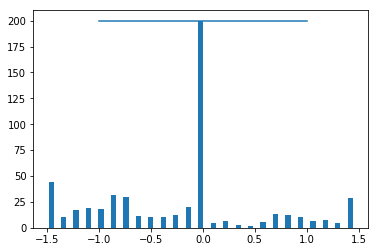
\includegraphics[scale=1]{Figures/bins.png}
 \caption{Diagram showing bins centered around zero degrees, meaning most of time car is driving straight. Binning diagrams for all datasets can be found in appendix B}
 \label{fig:bins-placeholder}
\end{figure}

\section{Training Log}

\begin{verbatim}
Run ID  Data       Network Acc. Error Saved Best Model 
3       log_sample NVIDIA1
\end{verbatim}

Run ID  Data    Network Training    Acc Error   Saved Best Model    Saved History
%1       Udacity 1       SGD Adam    .95 .06     model_01            history_01

\subsection{Run 3}

This model has a single output, steering angle, and produced very low accuracy.
Notes:
\begin{verbatim}
commit 423b5b783565b60e72f970485d9b3aa9887f5453
training time
dataset: sample_data
\end{verbatim}

\subsection{Run 4 - }

% Naoki's model not doing well, sanity check with one output
Also not doing well
Next run, 2 outputs (steering and throttle)

\subsection{Run 5 - 20201102081239} 

\begin{verbatim}
commit 076e8b32664738df6af9e14d75355504eb2a94b4
Much better results with two outputs. 
cat ../dataset/unity/log_sample/logs_Mon_Jul_13_08_29_01_2020/record_11659.json
Both are floats - steering angle and throttle
loss: 0.0105 - acc: 0.8502 - val_loss: 0.0111 - val_acc: 0.8617

dataset: sample_data
model: nvidia1
outputs: 2

Comment: Network trained with no augmentation of cropping.

\end{verbatim}

From this point onwards, a model name, if generated, is given with every run.

\subsection{Run 5 - 20201102090041\_nvidia2}
\begin{verbatim}
commit 42dabb6321ad25f667c8663b63412c88c96b3b38
model: nvidia2
outputs: 2
dataset: log_sample (size: 12k)
$ python train.py --model=nvidia2 --outdir=../trained_models
loss: 0.0108 - acc: 0.8483 - val_loss: 0.0117 - val_acc: 0.8495
\end{verbatim}

\subsection{Run 6 - 20201102094552\_nvidia1}
\begin{verbatim}
commit ec9d081b85f7386365428a73896b1d09be7ba917
model: nvidia1
outputs: 2
dataset: genRoad (280727)
command
$ train.py --model=nvidia1 --outdir=../trained_models
loss: 0.0077 - acc: 0.8726 - val_loss: 0.0077 - val_acc: 0.8732

Comment: Network trained with no augmentation of cropping.

video upload: https://youtu.be/ZLhrcyuONj0
\end{verbatim}

\subsection{Run 7 - 20201102090041\_nvidia2.h5}
\begin{verbatim}
commit 1da10b6745f583e180d5b9c5ba4874847ba8610c
model: nvidia2
outputs: 2
Dataset: genRoad
command
$ train.py --model=nvidia2 --outdir=../trained_models
\end{verbatim}

\subsection{Run 8 - 20201102134802\_nvidia2.h5}
\begin{verbatim}
commit 6960f2f5fb50b565c0dfd6c8fe3ac1d283192e69
model nvidia2
outputs 2
dataset log2
command:
train.py --model=nvidia2 --outdir=../trained_models
\end{verbatim}


\subsection{Run 9 - 20201102210514\_nvidia2.h5}
\begin{verbatim}
Running nvidia2 with augmentation
commit 6960f2f5fb50b565c0dfd6c8fe3ac1d283192e69
model nvidia2
outputs 2
dataset log2
command:
train.py --model=nvidia2 --outdir=../trained_models
loss: 0.0345 - acc: 0.7906 - val_loss: 0.0236 - val_acc: 0.8084
Stop! Still running!!! Epoch 60 and still improving. ...
% loss: 0.0193 - acc: 0.8250 - val_loss: 0.0116 - val_acc: 0.8503
% 0.0123 - acc: 0.8501 - val_loss: 0.0091 - val_acc: 0.8594
Ran 78 epochs and may have thrown error:
problems with loss graph
Note biggest increase in accuracy during training
\end{verbatim}

\subsection{Run 10 - 20201103211330\_nvidia2.h5}
\begin{verbatim}
Run nvidia2 WITHOUT augmentation, just preprocessing
commit 2add77bb60505fe25075f9da55f6465e65cd3825
model nvidia 2
outputs 2
dataset log2
command:
train.py --model=nvidia2 --outdir=../trained_models
loss: 0.0233 - acc: 0.8179 - val_loss: 0.0170 - val_acc: 0.8304
loss: 0.0084 - acc: 0.8656 - val_loss: 0.0086 - val_acc: 0.8655
Epoch 45/100
loss: 0.0083 - acc: 0.8662 - val_loss: 0.0086 - val_acc: 0.8638
problems with loss graph

No loss graph, again, no augmentation trained quicker that previous

\end{verbatim}

\subsection{Run 11}
\begin{verbatim}
commit 6439a8758d8b46a1cbc3bcefc9db4c15f70820df
model nvidia1
outputs 2
dataset log2
command:
train.py --model=nvidia1 --outdir=../trained_models
Epoch 1/100
1755/1755 [==============================] - 682s 389ms/step - loss: 0.0271 - acc: 0.8049 - val_loss: 0.0172 - val_acc: 0.8351
Epoch 84/100
1755/1755 [==============================] - 559s 318ms/step - loss: 0.0099 - acc: 0.8581 - val_loss: 0.0083 - val_acc: 0.8662
problems with loss graph (probably a bug introduced in adding info to graph?)

\end{verbatim}

\subsection{Run 12}
\begin{verbatim}
commit augment.ipynb
model nvidia_baseline
outputs 1
dataset log2 (280746)
command:
train.py --model=nvidia_baseline --outdir=../trained_models

There is an issue with the aspect ratio and cropping, need to investigate with augment.ipynb

Note log2 was renamed genRoad as it is exactly that and a more descriptive name.
ls
\end{verbatim}

\subsection{Run 13}
\begin{verbatim}
commit e14e4bb9bdd0d322867c6cdba706478f662e71f6
model nvidia_baseline
outputs 1
dataset log (45421)cd 
command:
train.py --model=nvidia_baseline
--outdir=../trained_models
--epochs=1
--inputs=../dataset/unity/log/*.jpg
--aug=True
--preproc=True

Comment: ran ok for one epoch, images sized correctly.
Adding more epochs
\end{verbatim}

\subsection{Run 14}
\begin{verbatim}
commit e14e4bb9bdd0d322867c6cdba706478f662e71f6
model nvidia_baseline
outputs 1
dataset log
command:
train.py --model=nvidia_baseline
--outdir=../trained_models
--epochs=100
--inputs=../dataset/unity/log/*.jpg
--aug=True
--preproc=True

Comment: Started with very low accuracy.
Stopped process as error seems to have gone out of range
Epoch 5/100
283/283 [==============================] 
- 107s 377ms/step - loss: nan - acc: 5.5259e-05 
- val_loss: nan - val_acc: 1.1004e-04
\end{verbatim}

\subsection{Run 15}
\begin{verbatim}
commit aec3290fdbc83e71e450deef650aa2d51873b886
model nvidia_baseline
outputs 2
dataset log
command:
train.py --model=nvidia_baseline
--outdir=../trained_models
--epochs=100
--inputs=../dataset/unity/log/*.jpg
--aug=True
--preproc=True
Comment: Started at loss: nan - acc: 0.4305. Two outputs definitely helps. Why?
Perhaps because model is not going around track at constant speed?

\end{verbatim}

\subsection{Run 16}

\begin{verbatim}
commit 10a3fc2f6d23e04f604914c1f8420e574a8ce808
model nvidia_baseline
outputs 2
dataset log
command:
train.py --model=nvidia_baseline
--outdir=../trained_models
--epochs=100
--inputs=../dataset/unity/log/*.jpg
--aug=True
--preproc=True
Comment: Added linear activation in final layer, loss returning a reasonable value:
loss: 1.2035 - acc: 0.5404
Turned into nan on 3rd epoch. Accuracy going down, stopping process
\end{verbatim}

\subsection{Run 17}

\begin{verbatim}
Commit: a76169106a9087f5cc7e851fe09294699bb6240c 
Model: nvidia_baseline
Outputs: 2
Dataset: genRoad
Command: 
train.py --model=nvidia_baseline
--outdir=../trained_models
--epochs=100
--inputs=../dataset/unity/log/*.jpg
--aug=True
--preproc=True

Comment: Removed weight decay
Still loss taking NaN values
Epoch 13/100
281/281 (...) val_loss: nan - val_acc: 0.4939

\end{verbatim}

\subsection{Run 18 }

\begin{verbatim}
Commit: baa8f3d066dc37d3c2bb7792fa9db4801824d1bb 
Model: nvidia_baseline
Outputs: 2
Dataset: genRoad
Command: 
train.py --model=nvidia_baseline
--outdir=../trained_models
--epochs=100
--inputs=../dataset/unity/log/*.jpg
--aug=True
--preproc=True
Comment: Removed dropout from last dense layer. Training loss NaN on first epoch.
Dropout added again, loss back to under 1. Seems to have an influence, trying
multiple dropout removals next.

\end{verbatim}



\subsection{Run 19}
\begin{verbatim}
Commit: 16a6f8ffc6399143e7ad5a6885ee9b44b3ca1dda
Model: nvidia_baseline
Outputs: 2
Dataset: genRoad
Command: 
train.py --model=nvidia_baseline
--outdir=../trained_models
--epochs=100
--inputs=../dataset/unity/log/*.jpg
--aug=True
--preproc=True
Comment: Left one dropout (.25) layer, loss still NaN.
\end{verbatim}

\subsection{Run 20}

\begin{verbatim}
Commit: d7e05ad1cdf0fab3a83975be259feb16830b5a38
Rest same as 19
Comment: Removed Dense(1164) layer. Loss is Nan on first epoch.
Stopping run

\end{verbatim}

\subsection{Run 21}
\begin{verbatim}
Commit: d8fb9705dd676554dcf84a213b3c27d0e1f9d0c4 
Rest same as 19
Comment: Loss is Nan on first epoch
Epoch 1/100
(...)loss: nan - acc: 0.5017
\end{verbatim}

\subsection{Run 22}
\begin{verbatim}
Commit: ba4432568a589eac5a7d7c4927fa96e2f9e11bd1
Model, Outputs, Dataset and Command: Same as 19
Comment: Using Glorot Uniform (Xavier) kernel initializer.
Loss in Nan on first epoch. Training stopped.
Epoch 1/100
284/284 [==============================] - 101s 357ms/step - loss: nan - acc: 0.4609
\end{verbatim}

\subsection{Run 23}
\begin{verbatim}
Commit: 5cba2c7b01a160e7053e09220e63b1c575cf51e8  
Model, Outputs, Dataset and Command: Same as 19
Comment: All biases initialized to 0.
Loss in Nan on first epoch. Training stopped.
Epoch 1/100
283/283 (...) loss: nan 
\end{verbatim}

\subsection{Run 24}
\begin{verbatim}
Commit: 56aea3e16bb0f9db5735dfa536809389f35b12da  
Model, Outputs, Dataset and Command: Same as 19
Comment: Removed Dense(10) layer
Loss in Nan on first epoch. Training stopped.
\end{verbatim}

\subsection{Run 25}
\begin{verbatim}
Commit: 6a8ee72727db2508d2ff1ae35d068837a5b524ab  
Model, Outputs, Dataset and Command: Same as 19
Comment: Increased dropout to 0.5.
Loss in Nan on second epoch. Training stopped.
Epoch 1/100
285/285 [==============================] - 100s 352ms/step 
- loss: 0.0660 - acc: 0.6910 - val_loss: 0.0299 - val_acc: 0.7809
Epoch 2/100
285/285 [==============================] - 100s 350ms/step - loss: nan - acc: 0.5000
\end{verbatim}

\subsection{Run 26}
\begin{verbatim}
Commit: e4a287dc816a2a4d2c47893b131c710b2ecb8594  
Model, Outputs, Dataset and Command: Same as 19
Comment: Spreading 0.5 dropout between layers (0.1 each).
Loss in Nan on third epoch. Training stopped.
Epoch 3/100
284/284 (...) loss: nan
\end{verbatim}

\subsection{Run 26}
\begin{verbatim}
Commit: 2e5bf1b7002a2ddbbe2fea003fce010627d723e2  
Model, Outputs, Dataset and Command: Same as 19
Comment: Changed layer dropout to 0.15.
Loss in Nan on first epoch. Training stopped.
\end{verbatim}

\subsection{Run 27}
\begin{verbatim}
Commit:   
Model, Outputs, Dataset and Command: Same as 19
Comment: Changed layer dropout to 0.05.
Loss in Nan on first epoch. Training stopped.
\end{verbatim}

\subsection{Run 28}
\begin{verbatim}
Commit: 9a70ff7e194736a475bdce0b6eddc65aad6ea8c0  
Model, Outputs, Dataset and Command: Same as 19
Comment: Changed number of kernels on 2nd Conv layer to 32.
Loss in Nan on first epoch. Training stopped.
\end{verbatim}

\subsection{Run 29}
\begin{verbatim}
Commit:   
Model, Outputs, Dataset and Command: Same as 19
Comment: Changed number of kernels on 3nd Conv layer to 64.
Loss in Nan on first epoch. Training stopped.
\end{verbatim}

\subsection{Run 30}
\begin{verbatim}
Commit: 1997b914e829466659a27bfe1b31a6a6374afd36  
Model, Outputs, Dataset and Command: Same as 19
Comment: Changed aspect ratio to 160x120
Loss in Nan on 2nd epoch. Training stopped.
Epoch 2/100
283/283 (...) loss: nan - acc: 0.5982
\end{verbatim}

\subsection{Run 31}
\begin{verbatim}
Commit: 1997b914e829466659a27bfe1b31a6a6374afd36  
Model, Outputs, Dataset and Command: Same as 19
Comment: Changed aspect ratio to 160x120
Loss in Nan on 2nd epoch. Training stopped.
Epoch 2/100
283/283 (...) loss: nan - acc: 0.5982
\end{verbatim}

\subsection{Run 32 - 20201117154210\_nvidia\_baseline.h5}
\begin{verbatim}
Commit: 1997b914e829466659a27bfe1b31a6a6374afd36  
Model: nvidia_baseline
Outputs: 2
Dataset: smallLoopingCourse (jungle1 renamed) (34443)
Command: 
train.py --model=nvidia_baseline
--outdir=../trained_models
--epochs=100
--inputs=../dataset/unity/genTrack/log/*.jpg
--aug=True
--preproc=True
Comment: Loss in Nan on 1st epoch. Training stopped.
This run also produced a usable model.
\end{verbatim}

\subsection{Run 33}
\begin{verbatim}
Commit: 861095ac1a997e0f460aca6ceda93df98b7d0a48  
Model, Outputs, Dataset and Command: Same as 19
Comment: Explicitly setting strides=(1,1) is conv layers 4 and 5.
Loss in Nan on 1st epoch. Training stopped.
\end{verbatim}

\subsection{Run 34 - 20201117162326\_nvidia\_baseline.h5}
\begin{verbatim}
Commit: d0b7160793ee433ed25724d966a7d3bd85ae8ffa  
Model, Outputs, Dataset and Command: Same as 19
Comment: Changed batch size to 64
Loss is NaN on 7th epoch
Epoch 7/100
567/567 (...) loss: nan

This run produced a usable model.
\end{verbatim}

This run consisted of a sanity check to determine if training would generate a loss value different from NaN (not a number). This was not the case as per results in comments.

\subsection{Run 35 - 20201120124421\_nvidia\_baseline.h5}
\begin{verbatim}
Commit: 1f5c64bc219b31cf8654d2cceec910f0dea5ecbf
Model: nvidia_baseline
Outputs: 2
Dataset: log_sample (12894 - small looping track)
Environment: simbox (local)
Command: 
--model=nvidia_baseline --outdir=../trained_models --epochs=100 --inputs=../dataset/unity/log_sample/*.jpg --aug=True --preproc=True

Comment: Sanity check run, with the aim of
establishing a repeatable training session, aiming
at debbugging Keras when the need arises, that is
when Keras is suspected of somehow having become 
corrupted. 

Note before running, all .jpg images were found to have corresponding steering angles:

$ python ~/git/sdsandbox/src/utils/jsonclean.py \
--inputs=/home/simbox/git/sdsandbox/dataset/unity/log_sample/*.jpg
Files deleted: 0

From the log file 20201120124421\_nvidia\_baseline.log:

Total training time: 0:03:09
Training loss: nan
Validation loss: nan
Training accuracy: 0.418
Validation accuracy: 0.480

Loss was NaN from 2nd training epoch:
Epoch 2/100
160/160 (...)- loss: nan

When running the model:

sudo ./Unity.AppImage --no-sandbox
And logging the session:
sudo tcpflow -i lo -c port 9091 > /tmp/tcpflow.log
and running predictions
python predict_client.py
--model=../trained_models/nvidia_baseline/20201120124421\_nvidia\_baseline.h5

The model was found to crash into a bollard. A video was generated using 
src/utils.MakeVideo.py

https://youtu.be/ZwP53IhBO20

\end{verbatim}

Given previous results, this run reverts code to commit 436f635f

%%%%%%%%%%%%%%%%%%%%%%%%%%%%%%%%%%%%%%%%%%%%%%%%%%%%%%%%%%%%%%%%%%%%%%%%%%%%%
% RUN 36
%%%%%%%%%%%%%%%%%%%%%%%%%%%%%%%%%%%%%%%%%%%%%%%%%%%%%%%%%%%%%%%%%%%%%%%%%%%%%
\subsection{Run 36 - 20201120171015\_sanity.h5}
(Referenced from \ref{results:net-training})
Long story short: Forensics are conducted in this run to find out what code generated model 
20201107210627\_nvidia1.h5, determining that outliers present in genRoad create problems. The outliers have since been quarantined.

\label{app_res:36}

\begin{verbatim}
Commit: 436f635fa183740832270ea7db6869918a786d55
Model: nvidia1
Outputs: 2
Dataset: log_sample (12894) 
Command: python train.py --model=sanity --outdir=../trained\_models
Environment: simbox
Comment: This model was trained with the committed code from November 7th, which produced the first success lap drive with not crashes or steering off the track.
There is no record of what commit generated the model, though on video:
https://youtu.be/9z0mMtOnUUc
One section in the video shows:
python predict_client.py \
--model=../trained_models/nvidia1/20201107210627\_nvidia1.h5
The model name contains date and time created.

The sanity check model trained in under five minutes, and the best model saved was
most likely (subject to double checking Keras source code) generated on the third epoch.

cat 20201120171015_sanity.log
Model name: ../trained_models/sanity/20201120171015_sanity.h5
Total training time: 0:04:38 (...)

A record of the training output is displayed below:

Epoch 1/100
80/80 [==============================] - 35s 432ms/step - loss: 0.0822 - acc: 0.6293 - val_loss: 0.0300 - val_acc: 0.8109
Epoch 2/100
80/80 [==============================] - 34s 425ms/step - loss: 0.0650 - acc: 0.7127 - val_loss: 0.0264 - val_acc: 0.8129
Epoch 3/100
80/80 [==============================] - 34s 423ms/step - loss: 0.0539 - acc: 0.7429 - val_loss: 0.0276 - val_acc: 0.8133
Epoch 4/100
80/80 [==============================] - 34s 424ms/step - loss: nan - acc: 0.5398 - val_loss: nan - val_acc: 0.4930
Epoch 5/100
80/80 [==============================] - 34s 427ms/step - loss: nan - acc: 0.4228 - val_loss: nan - val_acc: 0.4910
Epoch 6/100
80/80 [==============================] - 34s 428ms/step - loss: nan - acc: 0.4245 - val_loss: nan - val_acc: 0.4963
Epoch 7/100
80/80 [==============================] - 34s 431ms/step - loss: nan - acc: 0.4216 - val_loss: nan - val_acc: 0.4934
Epoch 8/100
80/80 [==============================] - 34s 428ms/step - loss: nan - acc: 0.4285 - val_loss: nan - val_acc: 0.4922

Further forensic examination of commits:

Trying to find what data and code generated model 20201107210627_nvidia1.h5
This was generated on November 7th. There are 4 commits for that day:

src(master)$ git log > gitlog.txt
src(master)$ vim gitlog.txt 
/Nov 7
ESC
:q

commit 436f635fa183740832270ea7db6869918a786d55 * commit used for this run
commit 9908eb32975fe33075fefad73f411896456b4a84 
commit 1ad187d4bff5b6936c065a1aaa15a654ef4d368c
commit 8ebd02ab9556a0c2869e9b551417a6e28d5f86cf

$ git diff master..436f635 train.py | grep "\-\-inputs"
-    parser.add_argument('--inputs', default='../dataset/unity/genRoad/log/*.jpg',
+    parser.add_argument('--inputs', default='../dataset/unity/log_sample/*.jpg', 

$ git diff master..9908eb3297 train.py | grep "\-\-inputs"
-    parser.add_argument('--inputs', default='../dataset/unity/genRoad/log/*.jpg' (...)
+    parser.add_argument('--inputs', default='../dataset/unity/log_sample/*.jpg' (...)

$ git diff master..1ad187d4b train.py | grep "\-\-inputs"
-    parser.add_argument('--inputs', default='../dataset/unity/genRoad/log/*.jpg'
+    parser.add_argument('--inputs', default='../dataset/unity/log2/*.jpg', 

$ git diff master..8ebd02ab train.py | grep "\-\-inputs"
-    parser.add_argument('--inputs', default='../dataset/unity/genRoad/log/*.jpg'
+    parser.add_argument('--inputs', default='../dataset/unity/log2/*.jpg',

The plus signal indicates lines added in the commit to the right, minus indicates what does
not exist in the commit to the right (9908eb3297) , where master is commit
436f635fa (current commit).

First two commits indicate log_sample dataset was used containing 38684 images files of
"small looping course" course
/log_sample(master)$ grep -nr jpg . | wc -l
38684
was used, 
second two commits indicate log2 dataset (renamed genRoad) containing 280747 image 
files on the "Generated Road" course.
/genRoad(master)$ grep -nr jpg . | wc -l
280747 (files)

The commits are listed in descending  chronological order, that is the first two datasets 
used to train on that day were log2 (later renamed genRoad), the following two datasets used were log_sample. The commit history suggests one of the two were used to generate
the Nov 7 successful model. Since the test was run on "Generated Track" course, and genRoad
contains images for "Generated Road" course, the assumption is sample_log dataset was used.

The sanity check model was then used to run predictions:
python predict_client.py --model=../trained_models/sanity/20201120171015_sanity.h5
(...)
connecting to 127.0.0.1 9091
fps 10.416671685462958
fps 10.405931675595545
fps 11.030877564739708
fps 11.092089084017463
fps 11.466601323987536
fps 11.362325028068517
fps 11.359920970581536
fps 10.861855550070638
fps 10.50113576298416
(...)

The tcpflow log was saved to:

tcpflow(master)$ ls
20201107210627_sanity_tcpflow.log

And a video generated (from /tmp copy) with script src/MakeVideo.py
$ python MakeVideo.py --filename=/tmp/tcpflow.log \ 
--model=20201120171015_sanity.h5 
and the video.avi output uploaded to https://youtu.be/JaSkkh-2xtI

Qualitatively (by observation) had a better lap than 20201107210627_nvidia1.h5 
(https://youtu.be/9z0mMtOnUUc) as it keeps to a single lane and the vehicle wheels
never touch the road markings

Noting that the prior predict_client.py fps logs indicate that frames-per-second at
varying ratios (e.g. fps 10.50113576298416), while MakeVideo.py records at 11 frames per second.
The video generated by MakeVideo.py is going around the track slightly faster
than the SDSandbox simulator steering with 20201120171015_sanity.h5 predictions.
between logged frames (tcpflow) and rendered frames (MakeVideo.py).
The frame rate logged with tcpflow is the frame rate SDSandbox is sending frames over 
the TCP network.

\end{verbatim}

%%%%%%%%%%%%%%%%%%%%%%%%%%%%%%%%%%%%%%%%%%%%%%%%%%%%%%%%%%%%%%%%%%%%%%%%%%%%%
% RUN 37
%%%%%%%%%%%%%%%%%%%%%%%%%%%%%%%%%%%%%%%%%%%%%%%%%%%%%%%%%%%%%%%%%%%%%%%%%%%%%
\subsection{Run 37 - 20201120184912\_sanity.h5}
Referenced from \ref{results:net-training} 
\label{app_res:37}
\begin{verbatim}
Commit: 1ad187d4bff5b6936c065a1aaa15a654ef4d368c
Model: nvidia1
Outputs: 2
Dataset: log2 (genRoad)
Command: python train.py --model=sanity --outdir=../trained\_models
Environment: simbox
Comment: This was the 3rd commit of the day
It seems that this has something to do with the dataset that was
being used. To be confirmed. Now running nvidia1 on genRoad
both on simbox and camber, loss still converging to 0
and not in NAN range. 

Training log:  ../trained_models/sanity/20201120184912\_sanity.log
Total training time: 16:08:01
Training loss: 0.010
Validation loss: 0.008
Training accuracy: 0.858
Validation accuracy: 0.858

This model took over 16 hours to train on 280727 images. It did not perform well.
Could it be due to the outliers?

$ sudo tcpflow -i lo -c port 9091 > /tmp/tcpflow.log
$ python predict_client.py --model=../trained_models/sanity/20201120184912_sanity.h5
$ python MakeVideo.py --filename=/tmp/tcpflow.log --model=20201120184912_sanity.h5

The angles were plotted using notebook GetSteeringAnglesFromtcpflow.ipynb
sa = GetSteeringFromtcpflow('../dataset/unity/genRoad/tcpflow/20201120184912_sanity.log')
sarr = np.asarray(sa)
p = sarr[:,0]
g = sarr[:,1]
plotSteeringAngles(p, g, 25, False, "Generated Road", "20201120184912_sanity.h5")

\end{verbatim}
%PAUSE HERE - WRITING FUNCTION TO PLOT STEERING ANGLES AND BINS FROM LOGS
Below are the normalized histogram and bins recovered from tcplow logs for model  
  
20201120184912\_sanity.h5 referenced in \ref{results:net-training}. The video generated from tcpflow log was uploaded to \href{https://youtu.be/xGDN8qOnv9M}{https://youtu.be/xGDN8qOnv9M}.

\begin{figure}[ht]
 \centering 
 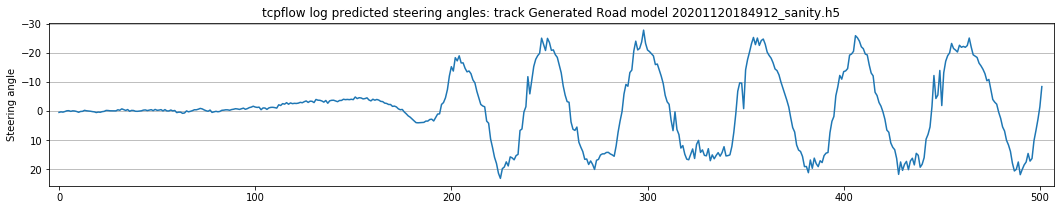
\includegraphics[width=\textwidth]{Figures/tcpflow_20201120184912_sanity_graph.png}
 \caption{Graph of steering angles recovered from tcpflow log genRoad/tcpflow/20201120184912\_sanity\_tcpflow.log for model 20201120184912\_sanity.h5 driving on Generated Road}
 \label{fig:tcpflow_20201120184912_graph}
\end{figure}

\begin{figure}[ht]
 \centering 
 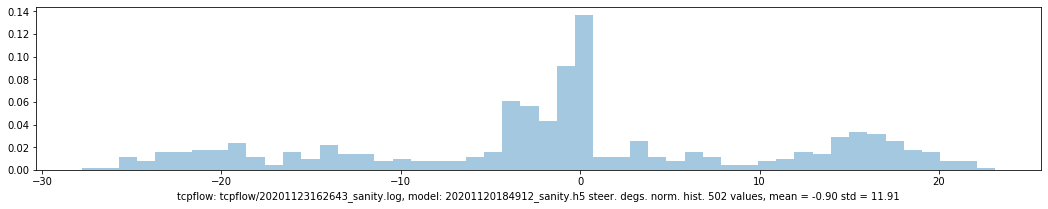
\includegraphics[width=\textwidth]{Figures/tcpflow_20201120184912_sanity_bins.png}
 \caption{Normalized histogram of tcpflow log genRoad/tcpflow/20201120184912\_ sanity \_ tcpflow.log for model 20201120184912\_ sanity.log driving on Generated Road}
 \label{fig:tcpflow_20201120184912_bins} 
\end{figure}

%%%%%%%%%%%%%%%%%%%%%%%%%%%%%%%%%%%%%%%%%%%%%%%%%%%%%%%%%%%%%%%%%%%%%%%%%%%%%
% RUN 38
%%%%%%%%%%%%%%%%%%%%%%%%%%%%%%%%%%%%%%%%%%%%%%%%%%%%%%%%%%%%%%%%%%%%%%%%%%%%%

\subsection{Run 38 - 20201123162643\_sanity.h5}
\begin{verbatim}
Commit: 1ad187d4bff5b6936c065a1aaa15a654ef4d368c
Model: nvidia1
Outputs: 2
Dataset: genRoad (clean - logs_Thu_Jul__9_16_00_15_2020 quarantined)
Command: python train.py --model=sanity --outdir=../trained\_models --epochs=5
NB Trained for 5 epochs
Environment: simbox
Comment: Rerunning commit 1ad187d4bf with cleaned data.
$ git checkout nov7 (this branch is commit 1ad187d4bff5b6936c065a1aaa15a654ef4d368c)
NB a simlink was created in unity/log2 pointing to unity/genRoad for the sake of
not changing committed source code.
ln -s ~/git/msc-data/unity/genRoad/ ~/git/msc-data/unity/log2

Epoch 1/5
1616/1616 [==============================] - 689s 427ms/step - loss: 0.0254 - acc: 0.8033 - val_loss: 0.0167 - val_acc: 0.8365
Epoch 2/5
1616/1616 [==============================] - 681s 421ms/step - loss: 0.0186 - acc: 0.8251 - val_loss: 0.0148 - val_acc: 0.8411
Epoch 3/5
1616/1616 [==============================] - 634s 393ms/step - loss: 0.0170 - acc: 0.8288 - val_loss: 0.0139 - val_acc: 0.8428
Epoch 4/5
1616/1616 [==============================] - 635s 393ms/step - loss: 0.0161 - acc: 0.8327 - val_loss: 0.0129 - val_acc: 0.8505
Epoch 5/5
1616/1616 [==============================] - 665s 411ms/step - loss: 0.0154 - acc: 0.8365 - val_loss: 0.0125 - val_acc: 0.8451

$ cat ../trained_models/sanity/20201123162643_sanity.log
Model name: ../trained_models/sanity/20201123162643_sanity.h5
Total training time: 0:55:10
Training loss: 0.015
Validation loss: 0.013
Training accuracy: 0.836
Validation accuracy: 0.845

The batch size used by generator function was 64:
src(nov7)$ cat train.py | grep batch
def generator(samples, is_training, batch_size=64):

Running the predictions:

$ sudo tcpflow -i lo -c port 9091 > /tmp/tcpflow.log
$ python predict_client.py --model=../trained_models/sanity/20201123162643\_sanity.h5
$ python MakeVideo.py --filename=/tmp/tcpflow.log --model=20201123162643\_sanity.h5
Video uploaded to https://youtu.be/uG2HvAbg2U4

tcpflow log file moved:
cp /tmp/tcpflow.log ../dataset/unity/genRoad/tcpflow/20201123162643_sanity.log

Plotting the bins with GetSteeringAnglesFromtcpflow.ipynb

sa = GetSteeringFromtcpflow('../dataset/unity/genRoad/tcpflow/20201123162643_sanity.log')
sarr = np.asarray(sa)
p = sarr[:,0]
p = sarr[:,0]  
plotSteeringAngles(p, g, 25, False, "Generated Road", "20201123162643_sanity.h5")
plotBinsFromArray(p, 25, "20201123162643_sanity.h5", "tcpflow/20201123162643_sanity.log") 
\end{verbatim}

Steering data recovered from tcpflow log genRoad/tcpflow/20201123162643\_sanity.log
This was running with commit 1ad187d4bf where frame \textbf{is not preprocessed} for prediction (predict\_ client.py) (Figures  \ref{fig:tcpflow_20201123162643_graph} and  \ref{fig:tcpflow_20201123162643_bins}). 

\begin{figure}[ht]
 \centering 
 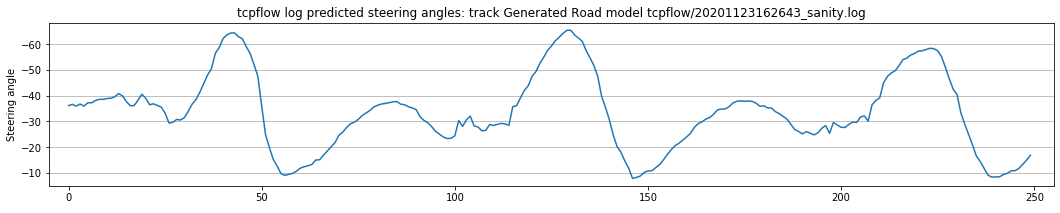
\includegraphics[width=\textwidth]{Figures/tcpflow_20201123162643_sanity_graph.png}
 \caption{Graph of steering angles recovered from tcpflow log genRoad/tcpflow/20201123162643\_sanity.log for model 20201123162643\_sanity.h5 driving on Generated Road}. The video can be seen here \href{https://youtu.be/uG2HvAbg2U4}{https://youtu.be/uG2HvAbg2U4}
 \label{fig:tcpflow_20201123162643_graph}
\end{figure}

\begin{figure}[ht]
 \centering 
 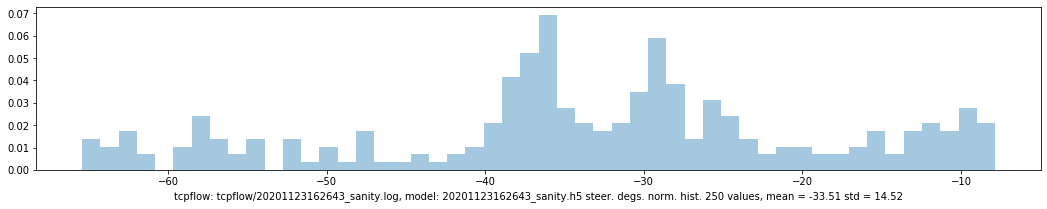
\includegraphics[width=\textwidth]{Figures/tcpflow_20201123162643_sanity_bins.png}
 \caption{Normalized histogram of tcpflow log genRoad/tcpflow/20201123162643\_ sanity.log for model 20201123162643\_ sanity.log driving on Generated Road}
 \label{fig:tcpflow_20201123162643_bins} 
\end{figure} 

%%%%%%%%%%%%%%%%%%%%%%%%%%%%%%%%%%%%%%%%%%%%%%%%%%%%%%%%%%%%%%%%%%%%%%%%%%%%%
% RUN 39
%%%%%%%%%%%%%%%%%%%%%%%%%%%%%%%%%%%%%%%%%%%%%%%%%%%%%%%%%%%%%%%%%%%%%%%%%%%%%
\subsection{Run 39 - 20201123162643\_sanity.h5}
\begin{verbatim}
Commit: 7f3086490118fec1a20e99e93cc1b853a91272b6
Model:  N/A (trained model)
Outputs:N/A (trained model)
Dataset: N/A (trained model)
Command: 
Environment: 
Comment: Same as previous run, but on branch 7f308649 (predict_client.py) with preprocessing

$ sudo tcpflow -i lo -c port 9091 (right angle bracket) /tmp/tcpflow.log
$ python predict_client.py --model=../trained_models/sanity/20201123162643\_sanity.h5
$ python MakeVideo.py --filename=/tmp/tcpflow.log --model=20201123162643\_sanity.h5

Link: https://youtu.be/377O2E_LwyU

tcpflow log file moved:
cp /tmp/tcpflow.log ../dataset/unity/genRoad/tcpflow/20201123162643_sanity_pp.log

sa = GetSteeringFromtcpflow('../dataset/unity/genRoad/tcpflow/20201123162643_sanity_pp.log')
sarr = np.asarray(sa)
p = sarr[:,0]
p = sarr[:,0]  
plotSteeringAngles(p, g, 25, False, "Generated Road", "20201123162643_sanity_pp.h5")
plotBinsFromArray(p, 25, "20201123162643_sanity.h5", "tcpflow/20201123162643_sanity_pp.log")

Video: https://youtu.be/377O2E_LwyU
\end{verbatim}

Steering data recovered from tcpflow log genRoad/tcpflow/20201123162643\_sanity\_pp.log
This was running with commit 7f308649 where frame \textbf{is preprocessed} for prediction (predict\_ client.py) (Figures  \ref{fig:tcpflow_20201123162643_pp_graph} and  \ref{fig:tcpflow_20201123162643_pp_bins}). 
Note the steering angles are a much tighter range. Bias toward positive 6 is due to road bending right.
The bins show a left skewed distribution, due to the right turn. Steering goes a bit crazy but model
manages to keep vehicle on the road.

\begin{figure}[ht]
 \centering 
 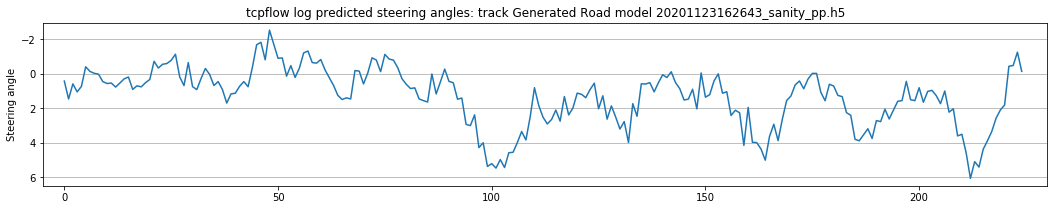
\includegraphics[width=\textwidth]{Figures/tcpflow_20201123162643_sanity_pp_graph.png}
 \caption{Graph of steering angles recovered from tcpflow log genRoad/tcpflow/20201123162643\_ sanity\_  pp.log for model 20201123162643\_ sanity.h5 driving on Generated Road}. The video can be seen here \href{https://youtu.be/377O2E\_ LwyU}{https://youtu.be/377O2E\_ LwyU}
 \label{fig:tcpflow_20201123162643_pp_graph}
\end{figure}

\begin{figure}[ht]
 \centering 
 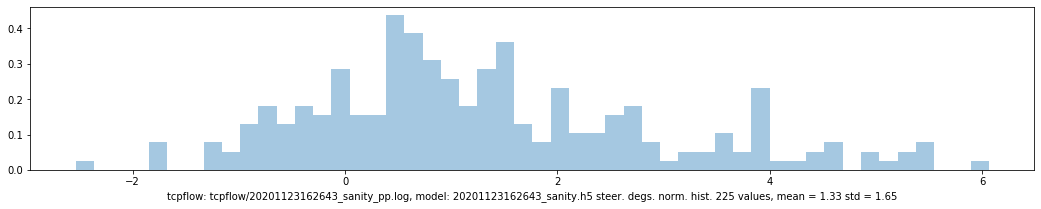
\includegraphics[width=\textwidth]{Figures/tcpflow_20201123162643_sanity_pp_bins.png}
 \caption{Normalized histogram of tcpflow log genRoad/tcpflow/20201123162643\_ sanity\_ pp.log for model 20201123162643\_sanity.h5 driving on Generated Road}
 \label{fig:tcpflow_20201123162643_pp_bins} 
\end{figure} 

%%%%%%%%%%%%%%%%%%%%%%%%%%%%%%%%%%%%%%%%%%%%%%%%%%%%%%%%%%%%%%%%%%%%%%%%%%%%%
% RUN 40
%%%%%%%%%%%%%%%%%%%%%%%%%%%%%%%%%%%%%%%%%%%%%%%%%%%%%%%%%%%%%%%%%%%%%%%%%%%%%
\subsection{Run 40 - 20201124032017\_ nvidia2.h5}
\begin{verbatim}
Commit: 7f3086490118fec1a20e99e93cc1b853a91272b6
Model: nvidia1
Outputs: 2
Dataset: N/A
Command: python3 train.py --model=nvidia2 --outdir=../trained_models --epochs=100
Environment: devcloud
Comment: Trained with nvidia2 model. Need to double check input size, as it might
be originally expecting 200x66.
Model did not do well and drove straight off the road. One thing to note, pixels are
being normalized and zero centered:
x = Lambda(lambda x: x/127.5 - 1.0)
Also, one single dropout layer. Need to try with different image size to match
original design.

$ sudo tcpflow -i lo -c port 9091 (right angle bracket) /tmp/tcpflow.log
$ python predict_client.py --model=../trained_models/devcloud/nvidia2/20201124032017_nvidia2.h5
$ python MakeVideo.py --filename=/tmp/tcpflow.log --model=20201124032017\_nvidia2.h5

https://youtu.be/RW-luOWQ_qY

tcpflow log file moved:
cp /tmp/tcpflow.log ../dataset/unity/genRoad/tcpflow/20201124032017_nvidia2.log

sa = GetSteeringFromtcpflow('../dataset/unity/genRoad/tcpflow/20201124032017_nvidia2.log)
sarr = np.asarray(sa)
p = sarr[:,0]
p = sarr[:,0]  
plotSteeringAngles(p, g, 25, False, "Generated Road", "20201124032017_nvidia2.h5")
plotBinsFromArray(p, 25, "20201124032017_nvidia2.h5", "tcpflow/20201124032017_nvidia2.log")
\end{verbatim}

Run 40 started well then pretty much drove straight off the road - need to investigate image
geometry
\begin{figure}[ht]
 \centering 
 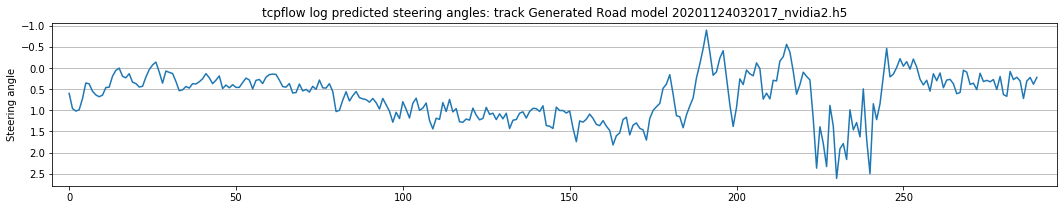
\includegraphics[width=\textwidth]{Figures/tcpflow_20201124032017_nvidia2_graph.png}
 \caption{Graph of steering angles recovered from tcpflow log genRoad/tcpflow/20201124032017\_ nvidia2.log for model 20201124032017\_ nvidia2.h5 driving on Generated Road}. The video can be seen here \href{https://youtu.be/RW-luOWQ\_ qY}{https://youtu.be/RW-luOWQ\_ qY}
 \label{fig:tcpflow_20201124032017_nvidia2_graph}
\end{figure}

\begin{figure}[ht]
 \centering 
 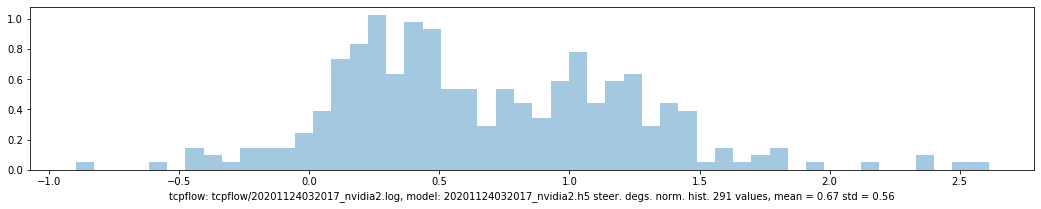
\includegraphics[width=\textwidth]{Figures/tcpflow_20201124032017_nvidia2_bins.png}
 \caption{Normalized histogram of tcpflow log genRoad/tcpflow/20201124032017\_ nvidia2.log for model 20201124032017\_ nvidia2.h5 driving on Generated Road}
 \label{fig:tcpflow_20201124032017_nvidia2_bins} 
\end{figure} 


%%%%%%%%%%%%%%%%%%%%%%%%%%%%%%%%%%%%%%%%%%%%%%%%%%%%%%%%%%%%%%%%%%%%%%%%%%%%%
% RUN 41
%%%%%%%%%%%%%%%%%%%%%%%%%%%%%%%%%%%%%%%%%%%%%%%%%%%%%%%%%%%%%%%%%%%%%%%%%%%%%
\subsection{Run 41 - 20201120171015\_ sanity.h5}
\label{app_res:41}
\label{}
\begin{verbatim}
Commit: f0d2513
Model: nvidia1
Outputs: 2
Dataset: log_sample (small looping circuit)

Command: 

$ sudo tcpflow -i lo -c port 9091 > /tmp/tcpflow_20201120171015_sanity.log
$ python predict_client.py --model=../trained_models/sanity/20201120171015_sanity.h5
$ python MakeVideo.py --filename=/tmp/tcpflow_20201120171015_sanity.log --model=20201120171015_sanity.h5
# mv
$ mv /tmp/tcpflow_20201120171015_sanity.log \ 
~/git/sdsandbox/trained_models/sanity/tcpflow/

Generating plot:
$ python steerlib.py
$ python 
>>> import steerlib as sl
>>> sa = sl.etSteeringFromtcpflow('../../dataset/unity/genRoad/tcpflow/tcpflow_20201120171015_sanity.log')
>>> sarr = np.asarray(sa)
>>> p = sarr[:,0]

plot = sl.plotSteeringAngles(p, None, 25, True, "Generated Track", "20201120171015_sanity.h5", 'tcpflow log predicted')
Environment: simbox
Comment: Prediction to generate tcpflow log
video https://youtu.be/LEmZJJzJkEE


\end{verbatim}

%%%%%%%%%%%%%%%%%%%%%%%%%%%%%%%%%%%%%%%%%%%%%%%%%%%%%%%%%%%%%%%%%%%%%%%%%%%%%
% RUN 42
%%%%%%%%%%%%%%%%%%%%%%%%%%%%%%%%%%%%%%%%%%%%%%%%%%%%%%%%%%%%%%%%%%%%%%%%%%%%%
\subsection{Run 42 - 20201120171015\_ sanity.h5}
\label{app_res:42}
\begin{verbatim}
Commit: 444c27f 
Model: Outputs: Dataset: Command: Environment: Same as run 41 
Comment: Testing conversion of PIL image to numpy array, bypassing saving .jpg to disk and reading from disk.

git diff ef4b48e..444c27f1 MakeVideo.py
diff --git a/src/utils/MakeVideo.py b/src/utils/MakeVideo.py
index f469471..8abd3c8 100644
--- a/src/utils/MakeVideo.py
+++ b/src/utils/MakeVideo.py
(...)
                     image = Image.open(BytesIO(base64.b64decode(imgString)))
+                    # try to convert to jpg
+                    image = np.array(image)
(...)



\end{verbatim}

Video still (Figure \ref{fig:tcpflow_Run42}) showing effect of converting PIL image directly to numpy array. Colour of sky is different.
No video was uploaded to youtube.


\begin{figure}[h!]
\centering
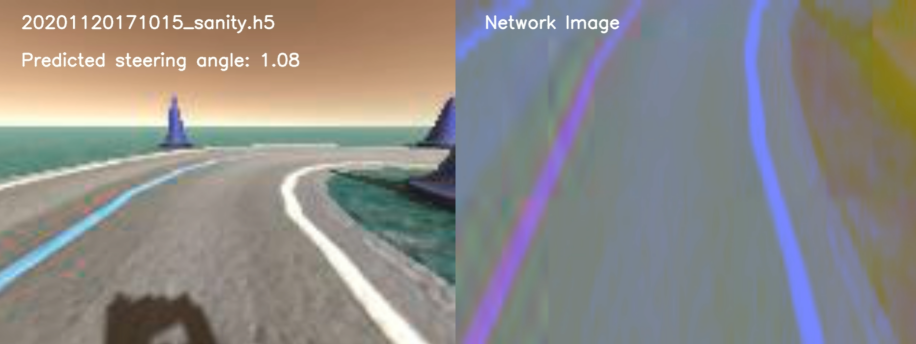
\includegraphics[width=\textwidth]{Figures/tcpflow_Run42.png}
\caption{tcpflow log image converted directly to numpy array (left) and image presented to network (right).}
\label{fig:tcpflow_Run42}
\end{figure}




%%%%%%%%%%%%%%%%%%%%%%%%%%%%%%%%%%%%%%%%%%%%%%%%%%%%%%%%%%%%%%%%%%%%%%%%%%%%%
% RUN 43
%%%%%%%%%%%%%%%%%%%%%%%%%%%%%%%%%%%%%%%%%%%%%%%%%%%%%%%%%%%%%%%%%%%%%%%%%%%%%
\subsection{Run 43 - Record triple video}
On this run we record a video with 3 frames side by side containing the simulator image, simulator image with added rain and the preprocessed image with added rain.

Interesting observation here (pending two tests to be documented), when we change the order of added rain, i.e. added to image before preprocesssing or added to image after preprocessing, this affects the outcome. Conclusion is currently pointing to the fact that moving image space from RGB to YUV is filtering out the rain "noise"

\label{app_res:43}
\begin{verbatim}
Commit: b0a77d2
Model: Outputs: Dataset: Environment: Same as run 41 
Command: 
$ python predict_client.py --model=../trained_models/sanity/20201120171015_sanity.h5 \ --rain=torrential --slant=20 --record=true

Video https://youtu.be/57jwwcjbfdE

Comment: As observed if noise is added to preprocessed image (at the point of being presented to network), sim crashes.

\end{verbatim}



%%%%%%%%%%%%%%%%%%%%%%%%%%%%%%%%%%%%%%%%%%%%%%%%%%%%%%%%%%%%%%%%%%%%%%%%%%%%%
% RUN 44
%%%%%%%%%%%%%%%%%%%%%%%%%%%%%%%%%%%%%%%%%%%%%%%%%%%%%%%%%%%%%%%%%%%%%%%%%%%%%
\subsection{Run 44 - Intensity x4}
\begin{verbatim}
Commit: 9696f3cee
Model: Outputs: Dataset: Environment: Same as run 41 
Command: 
$ python predict_client.py --model=../trained_models/sanity/20201120171015_sanity.h5 \
--rain=heavy --slant=20 --record=True

Comment: Changed luminosity multiply manually 
tcpflow file: (TODO plot steering including crash section)
~/git/sdsandbox/trained_models/sanity/tcpflow/20201120171015_sanity_run44.log

Video: https://youtu.be/UBd38Hlfv4w

\end{verbatim}


%%%%%%%%%%%%%%%%%%%%%%%%%%%%%%%%%%%%%%%%%%%%%%%%%%%%%%%%%%%%%%%%%%%%%%%%%%%%%
% RUN 45
%%%%%%%%%%%%%%%%%%%%%%%%%%%%%%%%%%%%%%%%%%%%%%%%%%%%%%%%%%%%%%%%%%%%%%%%%%%%%
\subsection{Run 45 - Intensity x8}
\begin{verbatim}
Commit: 20fe20c2e
Model: Outputs: Dataset: Environment: Same as run 41 
Command: 
$ python predict_client.py --model=../trained_models/sanity/20201120171015_sanity.h5 \
--rain=heavy --slant=20 --record=True
Comment: Changed intensity manually to 8, vehicle stays on road for 2 laps (stopped there).
Higher intensity means higher contrast between road and non-road, perhaps creating a 
guiding pattern.
It suggests there is some generalisation, as road is very unfamiliar.

tcpflow file:
~/git/sdsandbox/trained_models/sanity/tcpflow/20201120171015_sanity_run45.log

Video https://youtu.be/NerkRCSquiE
\end{verbatim}


%%%%%%%%%%%%%%%%%%%%%%%%%%%%%%%%%%%%%%%%%%%%%%%%%%%%%%%%%%%%%%%%%%%%%%%%%%%%%
% RUN 46
%%%%%%%%%%%%%%%%%%%%%%%%%%%%%%%%%%%%%%%%%%%%%%%%%%%%%%%%%%%%%%%%%%%%%%%%%%%%%
\subsection{Run 46 - 20201203164029\_ nvidia1.h5}
%\label{app_res:46}
\begin{verbatim}
Commit: 2d9e6983
Model: N/A
Outputs: N/A
Dataset: genTrack
Command: 
$ python train.py --model=nvidia1 --outdir=../trained_models --epochs=100 --inputs=../dataset/genTrackOneLap/*.jpg --aug=true --preproc=true --inputs=../dataset/unity/genTrack/*.jpg
Environment: devbox
Comment: Gathered dataset (35967 files) moved to ../dataset/unity/genTrack
ls -R | grep .jpg | wc -l
35967
Laps recorded with settings:
Max Speed 1.963599
Prop: 24
Diff: 5
Steer Max: 25
\end{verbatim}

%%%%%%%%%%%%%%%%%%%%%%%%%%%%%%%%%%%%%%%%%%%%%%%%%%%%%%%%%%%%%%%%%%%%%%%%%%%%%
% RUN 47
%%%%%%%%%%%%%%%%%%%%%%%%%%%%%%%%%%%%%%%%%%%%%%%%%%%%%%%%%%%%%%%%%%%%%%%%%%%%%
\subsection{Run 47 - 20201206171648\_ nvidia1.h5}
%\label{app_res:47}
\begin{verbatim}
Commit: 3f0622c8
Model: nvidia1
Outputs: 2
Dataset: genRoad
Command: python train.py
--model=nvidia1
--outdir=../trained_models
--epochs=5
--inputs=../dataset/unity/genRoad/*.jpg
--aug=True
--preproc=True
Environment: simbox
Comment: Created Augmentation class, handling image sizes for different models.
Then ran:
python predict_client.py --model=../trained_models/nvidia1/20201206171648_nvidia1.h5

When running this model (and possibly all previous):

$ python predict_client.py --model=../trained_models/nvidia1/20201206171648_nvidia1.h5

WARNING:tensorflow:Model was constructed with shape (None, 160, 120, 3) for input
Tensor("img_in:0", shape=(None, 160, 120, 3), dtype=float32), but it was called on an input
with incompatible shape (None, 120, 160, 3).

As it turns out, it was an assignment mess up. See diff on models.py between runs 48 and 49

Still the "flipped" input model did manage a stretch of Generated Road and surprisingly
manages to get around Generated Track, which is a total fluke, which may prove serendipitous.
\end{verbatim}


%%%%%%%%%%%%%%%%%%%%%%%%%%%%%%%%%%%%%%%%%%%%%%%%%%%%%%%%%%%%%%%%%%%%%%%%%%%%%
% RUN 48
%%%%%%%%%%%%%%%%%%%%%%%%%%%%%%%%%%%%%%%%%%%%%%%%%%%%%%%%%%%%%%%%%%%%%%%%%%%%%
\subsection{Run 48 - 20201206211122\_ nvidia1.h5}
%\label{app_res:48}
\begin{verbatim}
Commit: b5ad97f
Model: nvidia1
Outputs: 2
Dataset: genRoad
Command: python train.py
--model=nvidia1
--outdir=../trained_models
--epochs=5
--inputs=../dataset/unity/genRoad/*.jpg
--aug=True
--preproc=True
Environment: simbox
Comment: Based on previous (Run 47 warning), input to network was changed to col, row, channels. NB This was an oversight. In the next run, col, row remain, the assignement
changes (to fix mix-up).

This model did really well on Generated Road but not well at all on Generated Track.
\end{verbatim}

%%%%%%%%%%%%%%%%%%%%%%%%%%%%%%%%%%%%%%%%%%%%%%%%%%%%%%%%%%%%%%%%%%%%%%%%%%%%%
% RUN 49 - PROBABLY BEST NVIDIA1 MODEL
%%%%%%%%%%%%%%%%%%%%%%%%%%%%%%%%%%%%%%%%%%%%%%%%%%%%%%%%%%%%%%%%%%%%%%%%%%%%%
\subsection{Run 49 - 20201207091932\_ nvidia1.h5}
\label{app_res:49}
\begin{verbatim}
Commit: 55cb00b
Model: nvidia1
Outputs: 2
Dataset: genTrack
Command: 
$ python train.py
--model=nvidia1
--outdir=../trained_models
--epochs=5
--inputs=../dataset/unity/genTrack/*.jpg
--aug=True
--preproc=True

Environment: simbox
Comment: Trained for 5 epochs, maximum validation accuracy 0.7644. This model
drives both on Generated Road and Generated Track. This model took 1m23s to
train.

$ cat ../trained_models/nvidia1/20201207091932_nvidia1.log
Model name: ../trained_models/nvidia1/20201207091932_nvidia1.h5
Total training time: 0:01:23
Training loss: 0.021
Validation loss: 0.015
Training accuracy: 0.751
Validation accuracy: 0.757

Recording with no rain:
python predict_client.py
--model=../trained_models/nvidia1/20201207091932_nvidia1.h5 --record=True
https://youtu.be/S-PBNgJ_mdY

tcpflow log:
../trained_models/nvidia1/tcpflow/20201207091932_nvidia1_tcpflow.log

\end{verbatim}

Video of image plus network image - no rain - Generated Road:  
\url{https://youtu.be/S-PBNgJ_mdY} 

Figure \ref{fig:20201207091932_nvidia1_tcpflow} shows a slight positive value (road turning right) to start with, then a negative value (road turning left) steering angle.

\begin{figure}[ht]
 \centering 
 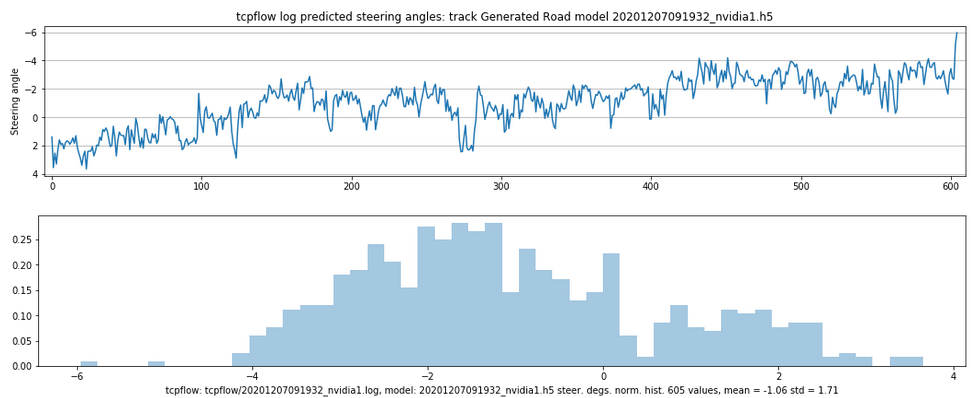
\includegraphics[width=\textwidth]{Figures/20201207091932_nvidia1_tcpflow.png}
 \caption{tcpflow steering angle log for model 20201207091932\_ nvidia1.h5 trained over 5 epochs on Generated Track, self-driving in a section of Generated Road}
 \label{fig:20201207091932_nvidia1_tcpflow}
\end{figure}

%%%%%%%%%%%%%%%%%%%%%%%%%%%%%%%%%%%%%%%%%%%%%%%%%%%%%%%%%%%%%%%%%%%%%%%%%%%%%
% RUN 50
%%%%%%%%%%%%%%%%%%%%%%%%%%%%%%%%%%%%%%%%%%%%%%%%%%%%%%%%%%%%%%%%%%%%%%%%%%%%%
\subsection{Run 50 - 20201207111940\_ nvidia2.h5}
%\label{app_res:50}
\begin{verbatim}
Commit: f9325ff
Model: nvidia2
Outputs: 2
Dataset: genTrack
Command: python train.py
--model=nvidia2
--outdir=../trained_models
--epochs=5
--inputs=../dataset/unity/genTrack/*.jpg
--aug=True
--preproc=True

Environment: simbox
Comment: Model trained with 0.5 dropout in a single layer. nvidia1 is trained
with 5 dropout layers at 0.1 each.

Running the model:
$ cd ~/Downloads
$ ./startunity.sh
$ sudo tcpflow -i lo -c port 9091 > /tmp/tcpflow.log
python predict_client.py
--model=../trained_models/nvidia2/20201207111940_nvidia2.h5
--modelname=nvidia2
--record=True

Video: https://youtu.be/b6IIoHuiUQ8

\end{verbatim}

Figure \ref{fig:20201207111940_nvidia2_tcpflow} shows a tcpflow of the nvidia2 model driving off the road by over-steering to the left after the first right turn as can be seen in video \url{https://youtu.be/b6IIoHuiUQ8} 

\begin{figure}[ht]
 \centering 
 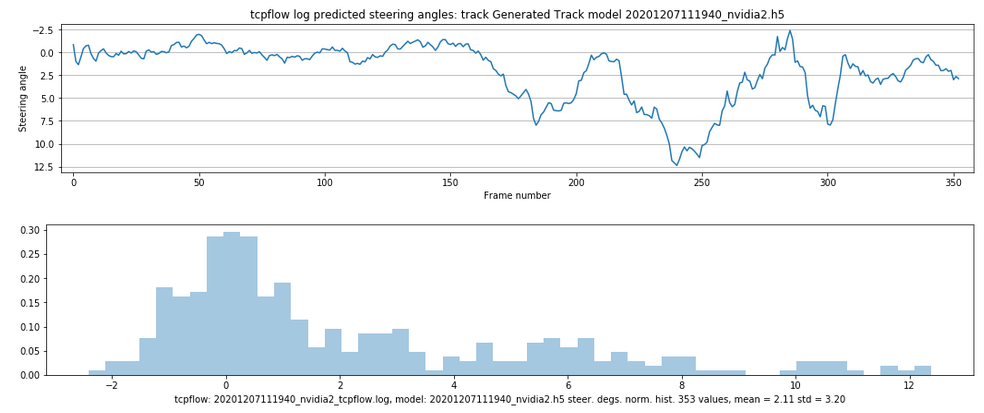
\includegraphics[width=\textwidth]{Figures/20201207111940_nvidia2_tcpflow.png}
 \caption{tcpflow steering angle log for model 20201207111940\_ nvidia2.h5 trained over 5 epochs on Generated Roard, self-driving off the road after first right turn.}
 \label{fig:20201207111940_nvidia2_tcpflow}
\end{figure}

%%%%%%%%%%%%%%%%%%%%%%%%%%%%%%%%%%%%%%%%%%%%%%%%%%%%%%%%%%%%%%%%%%%%%%%%%%%%%
% RUN 51
%%%%%%%%%%%%%%%%%%%%%%%%%%%%%%%%%%%%%%%%%%%%%%%%%%%%%%%%%%%%%%%%%%%%%%%%%%%%%
\subsection{Run 51 - 20201207124146\_ nvidia2.h5 }
%\label{app_res:51}
\begin{verbatim}
Commit: bb66ed7
Comment: Same as run 50, with dropout set to 0.25

$ python predict_client.py --model=../trained_models/nvidia2/20201207124146_nvidia2.h5 --modelname=nvidia2 --record=True

Video: https://youtu.be/-lDaiodokxw

\end{verbatim}

Figure \ref{fig:20201207124146_nvidia2_tcpflow} shows a tcpflow log of the nvidia2 model driving off the road by over-steering to the left off the first right turn as can be seen in video \url{https://youtu.be/-lDaiodokxw}. The model was trained with a single 0.25 dropout layer

\begin{figure}[ht]
 \centering 
 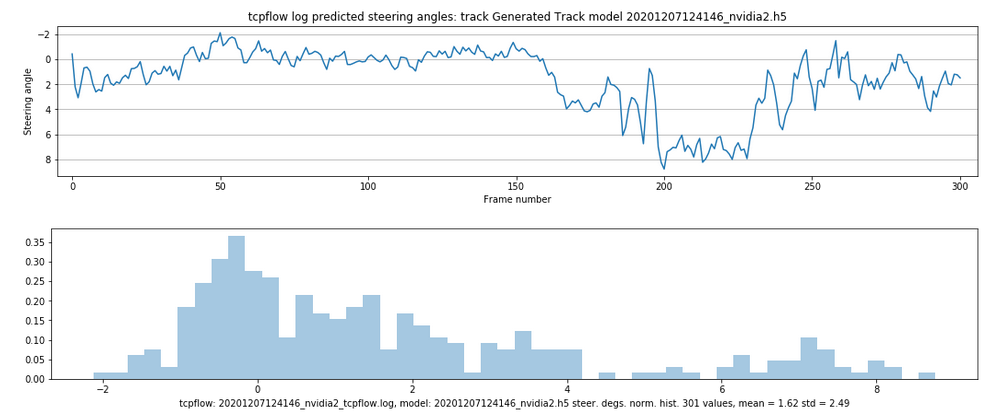
\includegraphics[width=\textwidth]{Figures/20201207124146_nvidia2_tcpflow.png}
 \caption{tcpflow steering angle log for model 20201207124146\_ nvidia2.h5 trained over 5 epochs on Generated Roard, self-driving off the road after first right turn.}
 \label{fig:20201207124146_nvidia2_tcpflow}
\end{figure}


%%%%%%%%%%%%%%%%%%%%%%%%%%%%%%%%%%%%%%%%%%%%%%%%%%%%%%%%%%%%%%%%%%%%%%%%%%%%%
% RUN 52
%%%%%%%%%%%%%%%%%%%%%%%%%%%%%%%%%%%%%%%%%%%%%%%%%%%%%%%%%%%%%%%%%%%%%%%%%%%%%
\subsection{Run 52 - 20201207132429\_ nvidia2.h5}
%\label{app_res:52}
\begin{verbatim}
Commit: cd3aa3a
Comment: Same as 51, with dropout set to 0.1

$ python predict_client.py 
--model=../trained_models/nvidia2/20201207132429_nvidia2.h5 
--modelname=nvidia2 --record=True

https://youtu.be/I6aB5RxYPsg

\end{verbatim}

Another case where nvidia2 drives off the road on the first right turn (Figure \ref{fig:20201207132429_nvidia2_tcpflow}). \url{https://youtu.be/I6aB5RxYPsg}.
\begin{figure}[ht]
 \centering 
 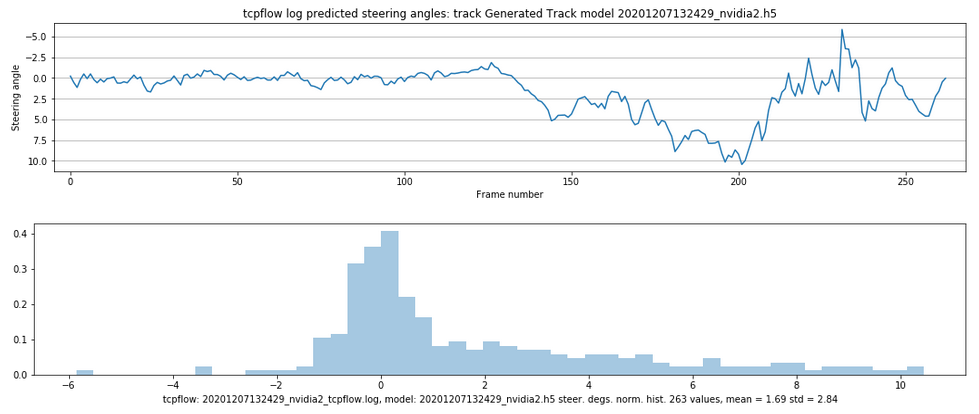
\includegraphics[width=\textwidth]{Figures/20201207132429_nvidia2_tcpflow.png}
 \caption{tcpflow steering angle log for model 220201207132429\_ nvidia2.h5 trained over 5 epochs on Generated Roard, self-driving off the road after first right turn.}
 \label{fig:220201207132429_nvidia2_tcpflow}
\end{figure}

%%%%%%%%%%%%%%%%%%%%%%%%%%%%%%%%%%%%%%%%%%%%%%%%%%%%%%%%%%%%%%%%%%%%%%%%%%%%%
% RUN 53
%%%%%%%%%%%%%%%%%%%%%%%%%%%%%%%%%%%%%%%%%%%%%%%%%%%%%%%%%%%%%%%%%%%%%%%%%%%%%
\subsection{Run 53 - 20201207133600\_ nvidia2.h5 }
%\label{app_res:XX}
\begin{verbatim}
Commit: 3e3ff1a
Comment: Same as 52
\end{verbatim}

Slightly better but still drives off road past the second left bollard.

The model:
\begin{verbatim}
_________________________________________________________________
Layer (type)                 Output Shape              Param #   
=================================================================
img_in (InputLayer)          [(None, 66, 200, 3)]      0         
_________________________________________________________________
lambda (Lambda)              (None, 66, 200, 3)        0         
_________________________________________________________________
conv2d_1 (Conv2D)            (None, 31, 98, 24)        1824      
_________________________________________________________________
conv2d_2 (Conv2D)            (None, 14, 47, 36)        21636     
_________________________________________________________________
conv2d_3 (Conv2D)            (None, 5, 22, 48)         43248     
_________________________________________________________________
conv2d_4 (Conv2D)            (None, 3, 20, 64)         27712     
_________________________________________________________________
conv2d_5 (Conv2D)            (None, 1, 18, 64)         36928     
_________________________________________________________________
dropout (Dropout)            (None, 1, 18, 64)         0         
_________________________________________________________________
flattened (Flatten)          (None, 1152)              0         
_________________________________________________________________
dense (Dense)                (None, 100)               115300    
_________________________________________________________________
dense_1 (Dense)              (None, 50)                5050      
_________________________________________________________________
steering_throttle (Dense)    (None, 2)                 102       
=================================================================
Total params: 251,800
Trainable params: 251,800
Non-trainable params: 0
_________________________________________________________________
[(None, 66, 200, 3)]    
\end{verbatim}

Video: \url{https://youtu.be/DPxFLukN0Ws}

%%%%%%%%%%%%%%%%%%%%%%%%%%%%%%%%%%%%%%%%%%%%%%%%%%%%%%%%%%%%%%%%%%%%%%%%%%%%%
% RUN 54
%%%%%%%%%%%%%%%%%%%%%%%%%%%%%%%%%%%%%%%%%%%%%%%%%%%%%%%%%%%%%%%%%%%%%%%%%%%%%
\subsection{Run 54 - 20201207141017\_ nvidia2.h5}
%\label{app_res:54}
\begin{verbatim}
Commit: a39008c
Comment: Same as run 53 except dropout layers added as per nvidia1.
Veers off road a little bit after run 53.

Video: https://youtu.be/SQQJacV622E
\end{verbatim}
Video: \url{https://youtu.be/SQQJacV622E}

Network:
\begin{verbatim}
import models
mymodel = models.nvidia_model2(2)
models.show_model_summary(mymodel)
Model: "model_1"
Layer (type)                 Output Shape              Param #   
=================================================================
img_in (InputLayer)          [(None, 66, 200, 3)]      0         
_________________________________________________________________
lambda (Lambda)              (None, 66, 200, 3)        0         
_________________________________________________________________
conv2d_1 (Conv2D)            (None, 31, 98, 24)        1824      
_________________________________________________________________
dropout (Dropout)            (None, 31, 98, 24)        0         
_________________________________________________________________
conv2d_2 (Conv2D)            (None, 14, 47, 36)        21636     
_________________________________________________________________
dropout_1 (Dropout)          (None, 14, 47, 36)        0         
_________________________________________________________________
conv2d_3 (Conv2D)            (None, 5, 22, 48)         43248     
_________________________________________________________________
dropout_2 (Dropout)          (None, 5, 22, 48)         0         
_________________________________________________________________
conv2d_4 (Conv2D)            (None, 3, 20, 64)         27712     
_________________________________________________________________
dropout_3 (Dropout)          (None, 3, 20, 64)         0         
_________________________________________________________________
conv2d_5 (Conv2D)            (None, 1, 18, 64)         36928     
_________________________________________________________________
dropout_4 (Dropout)          (None, 1, 18, 64)         0         
_________________________________________________________________
flattened (Flatten)          (None, 1152)              0         
_________________________________________________________________
dense (Dense)                (None, 100)               115300    
_________________________________________________________________
dense_1 (Dense)              (None, 50)                5050      
_________________________________________________________________
steering_throttle (Dense)    (None, 2)                 102       
=================================================================
Total params: 251,800
Trainable params: 251,800
Non-trainable params: 0
_________________________________________________________________
[(None, 66, 200, 3)]
(None, 66, 200, 3)
(None, 31, 98, 24)
(None, 31, 98, 24)
(None, 14, 47, 36)
(None, 14, 47, 36)
(None, 5, 22, 48)
(None, 5, 22, 48)
(None, 3, 20, 64)
(None, 3, 20, 64)
(None, 1, 18, 64)
(None, 1, 18, 64)
(None, 1152)
(None, 100)
(None, 50)
(None, 2)

\end{verbatim}

%%%%%%%%%%%%%%%%%%%%%%%%%%%%%%%%%%%%%%%%%%%%%%%%%%%%%%%%%%%%%%%%%%%%%%%%%%%%%
% RUN 55
%%%%%%%%%%%%%%%%%%%%%%%%%%%%%%%%%%%%%%%%%%%%%%%%%%%%%%%%%%%%%%%%%%%%%%%%%%%%%
\subsection{Run 55 - 20201207142129\_ nvidia2.h5}
%\label{app_res:55}
\begin{verbatim}
Commit: 28ea337
Comment: Same as 54, except aligned number of nvidia2 feature maps with nvidia1
\end{verbatim}
Another crash (\url{https://youtu.be/3ipZZgGtJUA}). Given that nvidia1 () run 52 did so well and every subsequent nvidia2 has crashed. Let's have a look at the actual crop we are presenting to both networks (Figure \ref{fig:2129x1932crops}):
 
\begin{figure}[ht]
 \centering 
 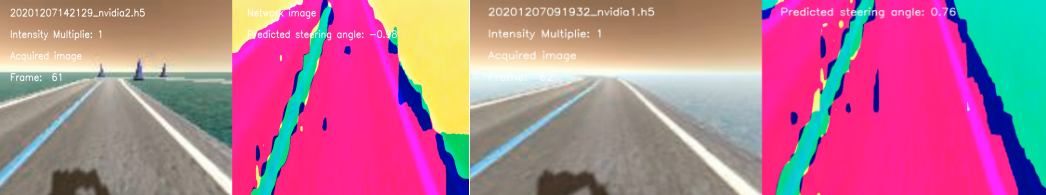
\includegraphics[width=\textwidth]{Figures/2129x1932crops.png}
 \caption{Network images presented to networks nvidia2 (20201207142129\_ nvidia2.h5) network (second from left) and nvidia1 (20201207091932\_ nvidia1.h5)}
 \label{fig:2129x1932crops}
\end{figure}

What is most noticeable is that the nvidia1 network image seems to somehow augment the road information, by making it cover more of the image.
If we look at the actual dimension crops up to commit 28ea337 on master branch, in conf.py:
\begin{verbatim}
# NVIDIA1
NVIDIA1 = 'nvidia1' # a.k.a. TawnNet
nvidia1_img_dims = [160,120,3,160,120,60,-25]
# NVIDIA2
NVIDIA2 = 'nvidia2' # a.k.a. NaokiNet
nvidia2_img_dims = [320,160,3,200,66,70,-35]
\end{verbatim}
where the last two digits on the list can be understood as the amount of top and bottom crop. In the case of nvidia1, for a total height of 120, a crop of index 60 till index (120 + (-25)) 95 (pixels) (total crop height = 35 pixels) is being made.
In the case of nvidia2, for a total height of 160 a crop of index 70 until index (160 + (-35)) 125 (total crop height = 55 pixels) is being made. 
In the case of nvidia1, the crop, as a proportion of the original image height is $35/120=0.21$.  
In the case of nvidia1, the crop, as a proportion of the original image height is $55/160=0.34$.
The bottom crop is the extent required to remove the vehicle shadow (if any) from the frame, so does not change. To change the top crop index (the conf.py IMG\_ TOP\_ CROP\_ IDX index value of nvidia2\_ img\_ dims) such that the proportion of both cropped images presented to networks nvidia1 and nvidia2 is the same, the top crop value of nvidia2 must change to approximately $x/160=0.21, x=34, tc=160-35-34=91$, where tc is the top crop value, that is, setting value of nvidia2\_ img\_ dims to
\begin{verbatim}
# NVIDIA2
NVIDIA2 = 'nvidia2' # a.k.a. NaokiNet
nvidia2_img_dims = [320,160,3,200,66,91,-35]
\end{verbatim}
Figure \ref{fig:nvidia1x1_nvidia2x3_crops} shows from left to right, the nvidia1 cropped image, followed by the nvidia2 cropped images with top crop value set to 70, 81 and 91 pixels. 
\begin{figure}[ht]
 \centering 
 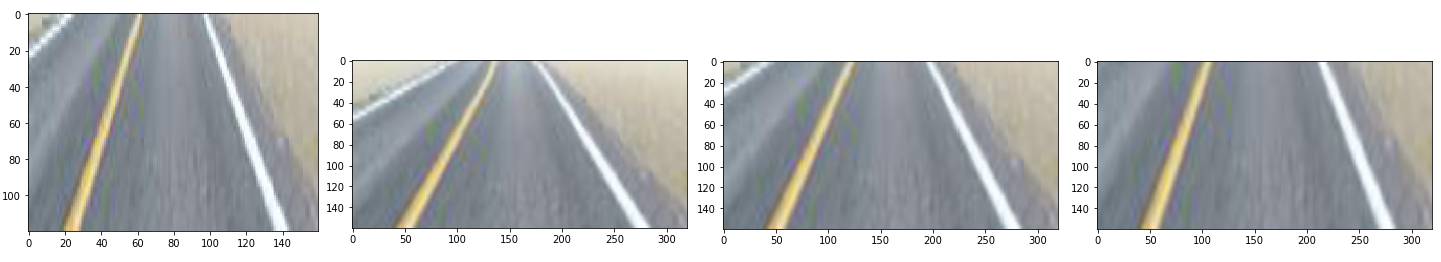
\includegraphics[width=\textwidth]{Figures/nvidia1x1_nvidia2x3_crops.png}
 \caption{Left to right, nvidia1 network crop, nvidia2 network crops at top crop set to 70, 81 and 91 pixels respectively)}
 \label{fig:nvidia1x1_nvidia2x3_crops}
\end{figure}

The network architecture for run 55, aligned with nvidia1 convolutional feature maps, is 24, 32, 64, 64 and 64 feature maps in the convolutional layers (conv2d\_ 1 through conv2d\_ 5):

\begin{verbatim}
_________________________________________________________________
Layer (type)                 Output Shape              Param #   
=================================================================
img_in (InputLayer)          [(None, 66, 200, 3)]      0         
_________________________________________________________________
lambda (Lambda)              (None, 66, 200, 3)        0         
_________________________________________________________________
conv2d_1 (Conv2D)            (None, 31, 98, 24)        1824      
_________________________________________________________________
dropout (Dropout)            (None, 31, 98, 24)        0         
_________________________________________________________________
conv2d_2 (Conv2D)            (None, 14, 47, 32)        19232     
_________________________________________________________________
dropout_1 (Dropout)          (None, 14, 47, 32)        0         
_________________________________________________________________
conv2d_3 (Conv2D)            (None, 5, 22, 64)         51264     
_________________________________________________________________
dropout_2 (Dropout)          (None, 5, 22, 64)         0         
_________________________________________________________________
conv2d_4 (Conv2D)            (None, 3, 20, 64)         36928     
_________________________________________________________________
dropout_3 (Dropout)          (None, 3, 20, 64)         0         
_________________________________________________________________
conv2d_5 (Conv2D)            (None, 1, 18, 64)         36928     
_________________________________________________________________
dropout_4 (Dropout)          (None, 1, 18, 64)         0         
_________________________________________________________________
flattened (Flatten)          (None, 1152)              0         
_________________________________________________________________
dense (Dense)                (None, 100)               115300    
_________________________________________________________________
dense_1 (Dense)              (None, 50)                5050      
_________________________________________________________________
steering_throttle (Dense)    (None, 2)                 102       
=================================================================
Total params: 266,628
Trainable params: 266,628
Non-trainable params: 0
_________________________________________________________________
[(None, 66, 200, 3)]
(None, 66, 200, 3)
(None, 31, 98, 24)
(None, 31, 98, 24)
(None, 14, 47, 32)
(None, 14, 47, 32)
(None, 5, 22, 64)
(None, 5, 22, 64)
(None, 3, 20, 64)
(None, 3, 20, 64)
(None, 1, 18, 64)
(None, 1, 18, 64)
(None, 1152)
(None, 100)
(None, 50)
(None, 2)    
\end{verbatim}

%%%%%%%%%%%%%%%%%%%%%%%%%%%%%%%%%%%%%%%%%%%%%%%%%%%%%%%%%%%%%%%%%%%%%%%%%%%%%
% RUN 56
%%%%%%%%%%%%%%%%%%%%%%%%%%%%%%%%%%%%%%%%%%%%%%%%%%%%%%%%%%%%%%%%%%%%%%%%%%%%%
\subsection{Run 56 - 20201207170938\_ nvidia2.h5}
%\label{app_res:56}
\begin{verbatim}
Commit: 8f163e9
Model: nvidia2
Outputs: 2
Dataset: genTrack
Command:

Environment: 
Comment: Changed top crop
https://youtu.be/I3gkoO1yWkk
\end{verbatim}

Another crash, changed top crop to 81 in conf.py.

%%%%%%%%%%%%%%%%%%%%%%%%%%%%%%%%%%%%%%%%%%%%%%%%%%%%%%%%%%%%%%%%%%%%%%%%%%%%%
% RUN 57
%%%%%%%%%%%%%%%%%%%%%%%%%%%%%%%%%%%%%%%%%%%%%%%%%%%%%%%%%%%%%%%%%%%%%%%%%%%%%
\subsection{Run 57 - 20201207175205\_ nvidia2.h5}
%\label{app_res:57}
\begin{verbatim}
Commit: 485d845
Model: nvidia2
Outputs: 2
Dataset: genTrack
Command:
python train.py
--model=nvidia2
--outdir=../trained_models
--epochs=5
--inputs=../dataset/unity/genTrack/*.jpg
--aug=True
--preproc=True

Environment: simbox
Comment: Same as run 56, done as sanity check. Might have messed up the 
predict_client.py parameters in 56. This model almost goes off the track on the first corner but actually gets around the track and works with a 81 top crop.

python predict_client.py 
--model=../trained_models/nvidia2/20201207175205_nvidia2.h5 
--modelname=nvidia2 --record=True --modelname=nvidia2
\end{verbatim}

This actually managed to get around the track (\url{https://youtu.be/Vqd2W39CwdA}

%%%%%%%%%%%%%%%%%%%%%%%%%%%%%%%%%%%%%%%%%%%%%%%%%%%%%%%%%%%%%%%%%%%%%%%%%%%%%
% RUN 58
%%%%%%%%%%%%%%%%%%%%%%%%%%%%%%%%%%%%%%%%%%%%%%%%%%%%%%%%%%%%%%%%%%%%%%%%%%%%%
\subsection{Run 58 - 20201207184329\_ nvidia2.h5}
%\label{app_res:58}
\begin{verbatim}
Commit: 196f820
Model: nvidia2
Outputs: 2
Dataset: genTrack
Command:
python train.py 
--model=nvidia2
--outdir=../trained_models
--epochs=5
--inputs=../dataset/unity/genTrack/*.jpg
--aug=True
--preproc=True
Environment: simbox
Comment: top crop set to 77. 
Model drove off the road.

Inference time prediction:

$ python predict_client.py ../trained_models/nvidia2/20201207184329_nvidia2.h5 --modelname=nvidia2 --record=True --modelname=nvidia2
\end{verbatim}

Top crop set to 77, drove off the road (\url{https://youtu.be/jHWX7bi5Okw}).


%%%%%%%%%%%%%%%%%%%%%%%%%%%%%%%%%%%%%%%%%%%%%%%%%%%%%%%%%%%%%%%%%%%%%%%%%%%%%
% RUN 59
%%%%%%%%%%%%%%%%%%%%%%%%%%%%%%%%%%%%%%%%%%%%%%%%%%%%%%%%%%%%%%%%%%%%%%%%%%%%%
\subsection{Run 58 - 20201207185525\_ nvidia2.h5}
%\label{app_res:58}
\begin{verbatim}
Commit: 0cc41e7
Model: nvidia2
Outputs: 2
Dataset: genTrack   
Command:
python train.py 
--model=nvidia2
--outdir=../trained_models
--epochs=5
--inputs=../dataset/unity/genTrack/*.jpg
--aug=True
--preproc=True
Environment: simbox

Comment: top crop set to 83. Drove off the road

$ python predict_client.py 
--model=../trained_models/nvidia2/20201207185525_nvidia2.h5 --modelname=nvidia2 
--record=True --modelname=nvidia2

\end{verbatim}
\url{https://youtu.be/dkV0Tbfwr9Q}


f1a5263

%%%%%%%%%%%%%%%%%%%%%%%%%%%%%%%%%%%%%%%%%%%%%%%%%%%%%%%%%%%%%%%%%%%%%%%%%%%%%
% RUN 60
%%%%%%%%%%%%%%%%%%%%%%%%%%%%%%%%%%%%%%%%%%%%%%%%%%%%%%%%%%%%%%%%%%%%%%%%%%%%%
\subsection{Run 60 - 20201207190447\_ nvidia2.h5}
%\label{app_res:60}
\begin{verbatim}
Commit: f1a5263
Model:  Same as 59
Outputs:  Same as 59
Dataset:  Same as 59
Command: Same as 59

Environment: simbox
Comment: Crash

Prediction:
$ python predict_client.py 
--model=../trained_models/nvidia2/20201207190447_nvidia2.h5 --modelname=nvidia2 
--record=True --modelname=nvidia2
\end{verbatim}

%%%%%%%%%%%%%%%%%%%%%%%%%%%%%%%%%%%%%%%%%%%%%%%%%%%%%%%%%%%%%%%%%%%%%%%%%%%%%
% RUN 61
%%%%%%%%%%%%%%%%%%%%%%%%%%%%%%%%%%%%%%%%%%%%%%%%%%%%%%%%%%%%%%%%%%%%%%%%%%%%%
\subsection{Run 61 - 20201207192309\_ nvidia2.h5 }
%\label{app_res:XX}
\begin{verbatim}
Commit: ae4742b
Model:  Same as 59
Outputs:  Same as 59
Dataset:  Same as 59
Command: Same as 59
Comment: Not zero centering pixel values, just normalizing.
\end{verbatim}
\url{https://youtu.be/5VnNHD0wgFc}


%%%%%%%%%%%%%%%%%%%%%%%%%%%%%%%%%%%%%%%%%%%%%%%%%%%%%%%%%%%%%%%%%%%%%%%%%%%%%
% RUN 62 - One of the best nvidia2 architecture models
%%%%%%%%%%%%%%%%%%%%%%%%%%%%%%%%%%%%%%%%%%%%%%%%%%%%%%%%%%%%%%%%%%%%%%%%%%%%%
\subsection{Run62 - 20201207192948\_ nvidia2.h5}
%\label{app_res:62}
\begin{verbatim}
Commit: df953d2
Model:  Same as 59
Outputs:  Same as 59
Dataset:  Same as 59
Command: Same as 59
Environment: same as 59
Comment: Restore last 10 unit fully connected layer. This one drives well around Generated Track.

$ python predict_client.py 
--model=../trained_models/nvidia2/20201207192948_nvidia2.h5 --modelname=nvidia2 
--record=True --modelname=nvidia2
\end{verbatim}
\url{https://youtu.be/7-Paz1_PKAo}

%%%%%%%%%%%%%%%%%%%%%%%%%%%%%%%%%%%%%%%%%%%%%%%%%%%%%%%%%%%%%%%%%%%%%%%%%%%%%
% RUN 63
%%%%%%%%%%%%%%%%%%%%%%%%%%%%%%%%%%%%%%%%%%%%%%%%%%%%%%%%%%%%%%%%%%%%%%%%%%%%%
\subsection{Run 63 - 20201207193607\_ nvidia2.h5}
%\label{app_res:63}
\begin{verbatim}
Commit: 3f65201
Model:  Same as 59
Outputs:  Same as 59
Dataset:  Same as 59
Command: Same as 59
Environment: same as 59 
Comment: Only one dropout layer as per original NaokiNet model. Seems to be
getting around the track ok. Very smooth. Comparable to run 62.

$ python predict_client.py 
--model=../trained_models/nvidia2/20201207193607_nvidia2.h5 --modelname=nvidia2 
--record=True --modelname=nvidia2

\end{verbatim}
\url{https://youtu.be/MRDp-eAAt18}
%%%%%%%%%%%%%%%%%%%%%%%%%%%%%%%%%%%%%%%%%%%%%%%%%%%%%%%%%%%%%%%%%%%%%%%%%%%%%
% RUN 64
%%%%%%%%%%%%%%%%%%%%%%%%%%%%%%%%%%%%%%%%%%%%%%%%%%%%%%%%%%%%%%%%%%%%%%%%%%%%%
\subsection{Run 64 - 20201207194331\_ nvidia2.h5}
%\label{app_res:64}
\begin{verbatim}
commit: 3cc0a1bfb8
Model:  Same as 59
Outputs:  Same as 59
Dataset:  Same as 59
Command: Same as 59
Environment: same as 59 
Comment: No Dropout layers

$ python predict_client.py --model=../trained_models/nvidia2/20201207194331_nvidia2.h5 --modelname=nvidia2 --record=True --modelname=nvidia2

\end{verbatim}
\url{https://youtu.be/jHhszDocnu4}


%%%%%%%%%%%%%%%%%%%%%%%%%%%%%%%%%%%%%%%%%%%%%%%%%%%%%%%%%%%%%%%%%%%%%%%%%%%%%
% RUN 65
%%%%%%%%%%%%%%%%%%%%%%%%%%%%%%%%%%%%%%%%%%%%%%%%%%%%%%%%%%%%%%%%%%%%%%%%%%%%%
\subsection{Run 65 - 20201207194331\_ nvidia2.h5 }
%\label{app_res:65}
\begin{verbatim}
Comment: Model 65 on Generated Road - handles ok-ish-ish
\end{verbatim}
\url{https://youtu.be/WA2uLtRn3Z0}

%%%%%%%%%%%%%%%%%%%%%%%%%%%%%%%%%%%%%%%%%%%%%%%%%%%%%%%%%%%%%%%%%%%%%%%%%%%%%
% RUN 66
%%%%%%%%%%%%%%%%%%%%%%%%%%%%%%%%%%%%%%%%%%%%%%%%%%%%%%%%%%%%%%%%%%%%%%%%%%%%%
\subsection{Run 66 - 20201207193607\_ nvidia2.h5}
%\label{app_res:65}
\begin{verbatim}
Comment: Model 64 (only one dropout layer) on Generated Road. Also a bit wobbly but manages to stay on the road for a while (drop off in the end).
\end{verbatim}
\url{https://youtu.be/WA2uLtRn3Z0}


%%%%%%%%%%%%%%%%%%%%%%%%%%%%%%%%%%%%%%%%%%%%%%%%%%%%%%%%%%%%%%%%%%%%%%%%%%%%%
% RUN 67
%%%%%%%%%%%%%%%%%%%%%%%%%%%%%%%%%%%%%%%%%%%%%%%%%%%%%%%%%%%%%%%%%%%%%%%%%%%%%
\subsection{Run 67 - 20201207195804\_ nvidia2.h5}
%\label{app_res:XX}
\begin{verbatim}
Commit: 957d14c
Model:  Same as 59
Outputs:  Same as 59
Dataset:  Same as 59
Command: Same as 59
Environment: same as 59 
Comment: zero centered pixel values, drove off the road. This seems to be
the change that most impacts model performance, followed by image size.

Prediction:
$ python predict_client.py --model=../trained_models/nvidia2/20201207195804_nvidia2.h5 --modelname=nvidia2 --record=True --modelname=nvidia2

\end{verbatim}
\url{https://youtu.be/ZSgKMGL7azY}

%%%%%%%%%%%%%%%%%%%%%%%%%%%%%%%%%%%%%%%%%%%%%%%%%%%%%%%%%%%%%%%%%%%%%%%%%%%%%
% RUN 68
%%%%%%%%%%%%%%%%%%%%%%%%%%%%%%%%%%%%%%%%%%%%%%%%%%%%%%%%%%%%%%%%%%%%%%%%%%%%%
\subsection{Run 68 - 20201207201157\_ nvidia\_ baseline.h5 }
%\label{app_res:68}
\begin{verbatim}
Commit: b1af57c
Model: nvidia_baseline
Outputs: 2
Dataset: genTrack
Command:
python train.py
--model=nvidia_baseline
--outdir=../trained_models
--epochs=5
--inputs=../dataset/unity/genTrack/*.jpg
--aug=True
--preproc=True
Environment: simbox
Comment: Drove off the road. Looks like geometry of input image must be known.
\end{verbatim}
\url{https://youtu.be/RxcC9tHCVUo}



%%%%%%%%%%%%%%%%%%%%%%%%%%%%%%%%%%%%%%%%%%%%%%%%%%%%%%%%%%%%%%%%%%%%%%%%%%%%%
% RUN 69
%%%%%%%%%%%%%%%%%%%%%%%%%%%%%%%%%%%%%%%%%%%%%%%%%%%%%%%%%%%%%%%%%%%%%%%%%%%%%
\subsection{Run 69 - }
%\label{app_res:69}
\begin{verbatim}
Commit: 4831a1b
Model: nvidia2
Outputs: 2
Dataset: genTrack
Command:
python train.py
--model=nvidia2
--outdir=../trained_models
--epochs=5
--inputs=../dataset/unity/genTrack/*.jpg
--aug=True
--preproc=True
Environment: simbox
Comment: set second convolutional layer to 32 feature maps failed to predict.

    ValueError: Input 0 of layer dense is incompatible with the layer: expected axis -1 of input shape to have value 6656 but received input with shape [None, 1152]

Was still zero centering (sanity checking)

$ python predict_client.py --model=../trained_models/nvidia2/20201102090041_nvidia2.h5  --record=True --modelname=nvidia2


\end{verbatim}

%%%%%%%%%%%%%%%%%%%%%%%%%%%%%%%%%%%%%%%%%%%%%%%%%%%%%%%%%%%%%%%%%%%%%%%%%%%%%
% RUN 70
%%%%%%%%%%%%%%%%%%%%%%%%%%%%%%%%%%%%%%%%%%%%%%%%%%%%%%%%%%%%%%%%%%%%%%%%%%%%%
\subsection{Run 70 - 20201207203451\_ nvidia2.h5 }
%\label{app_res:XX}
\begin{verbatim}
Commit: 5e313d6 
Model: nvidia2
Outputs: 2
Dataset: genTrack   
Command:
python train.py
--model=nvidia2
--outdir=../trained_models
--epochs=5
--inputs=../dataset/unity/genTrack/*.jpg
--aug=True
--preproc=True

Environment: simbox
Comment: Weird how a change in feature map size changes model performance. It is still going ok but not the best.

$ python predict_client.py --model=../trained_models/nvidia2/20201207203451_nvidia2.h5  --record=True --modelname=nvidia2

\end{verbatim}
\url{https://youtu.be/3h_Lp3gtHnw}

%%%%%%%%%%%%%%%%%%%%%%%%%%%%%%%%%%%%%%%%%%%%%%%%%%%%%%%%%%%%%%%%%%%%%%%%%%%%%
% RUN 71 
%%%%%%%%%%%%%%%%%%%%%%%%%%%%%%%%%%%%%%%%%%%%%%%%%%%%%%%%%%%%%%%%%%%%%%%%%%%%%
\subsection{Run 71 - }
%\label{app_res:XX}
\begin{verbatim}
Commit: bc76eb3 
Model: alexnet
Outputs: 2 
Dataset: genTrack
Command:
python train.py
--model=alexnet
--outdir=../trained_models
--epochs=5
--inputs=../dataset/unity/genTrack/*.jpg
--aug=True
--preproc=True

Environment: 
Comment: Error - Input to reshape is a tensor with 495616 values, but the
requested shape requires a multiple of 6336. Need to sort out shapes.
\end{verbatim}

%%%%%%%%%%%%%%%%%%%%%%%%%%%%%%%%%%%%%%%%%%%%%%%%%%%%%%%%%%%%%%%%%%%%%%%%%%%%%
% RUN 72
%%%%%%%%%%%%%%%%%%%%%%%%%%%%%%%%%%%%%%%%%%%%%%%%%%%%%%%%%%%%%%%%%%%%%%%%%%%%%
\subsection{Run 72 - 20201207091932\_ nvidia1.h5 }
%\label{app_res:72}
\begin{verbatim}
Commit: bc76eb3 
Model: nvidia1
Outputs: 2
Dataset: genTrack
Command:
sudo tcpflow -i lo -c port 9091 >
/tmp/20201207091932_nvidia1_light_rain_mult_1_tcpflow.log

$ python predict_client.py
--model=../trained_models/nvidia1/20201207091932_nvidia1.h5 --modelname=nvidia1
--rain='light' --slant=0 --record=True

Environment: simbox
Comment: light rain


\end{verbatim}
\url{https://youtu.be/V5GrdPGTPZs}

%%%%%%%%%%%%%%%%%%%%%%%%%%%%%%%%%%%%%%%%%%%%%%%%%%%%%%%%%%%%%%%%%%%%%%%%%%%%%
% RUN 73
%%%%%%%%%%%%%%%%%%%%%%%%%%%%%%%%%%%%%%%%%%%%%%%%%%%%%%%%%%%%%%%%%%%%%%%%%%%%%
\subsection{Run 73 - 20201207091932\_ nvidia1.h5}
%\label{app_res:73}
\begin{verbatim}
Commit: bc76eb3 
Model: nvidia1
Outputs: 2
Dataset: genTrack
Command:
sudo tcpflow -i lo -c port 9091 >
/tmp/20201207091932_nvidia1_heavy_10_mult_1_tcpflow.log

$ python predict_client.py
--model=../trained_models/nvidia1/20201207091932_nvidia1.h5 --modelname=nvidia1
--rain='heavy' --slant=10 --record=True

Environment: simbox
Comment: heavy rain 10 degree slant
\end{verbatim}
\url{https://youtu.be/Yff1s3RYFSg}

%%%%%%%%%%%%%%%%%%%%%%%%%%%%%%%%%%%%%%%%%%%%%%%%%%%%%%%%%%%%%%%%%%%%%%%%%%%%%
% RUN 74
%%%%%%%%%%%%%%%%%%%%%%%%%%%%%%%%%%%%%%%%%%%%%%%%%%%%%%%%%%%%%%%%%%%%%%%%%%%%%
\subsection{Run 74 - 20201207091932\_ nvidia1.h5}
%\label{app_res:74}
\begin{verbatim}
Commit: 
Model: 
Outputs: 
Dataset: 
Command:
sudo tcpflow -i lo -c port 9091 >
/tmp/20201207091932_nvidia1_torrential_20__mult_1_tcpflow.log

$ python predict_client.py
--model=../trained_models/nvidia1/20201207091932_nvidia1.h5 --modelname=nvidia1
--rain='torrential' --slant=20 --record=True

Environment: simbox
Comment: Torrential rain, 20 degree slant
\end{verbatim}
\url{https://youtu.be/Hn4fXr1a89I}


%%%%%%%%%%%%%%%%%%%%%%%%%%%%%%%%%%%%%%%%%%%%%%%%%%%%%%%%%%%%%%%%%%%%%%%%%%%%%
% RUN 75
%%%%%%%%%%%%%%%%%%%%%%%%%%%%%%%%%%%%%%%%%%%%%%%%%%%%%%%%%%%%%%%%%%%%%%%%%%%%%
\subsection{Run 75 - 20201207091932\_ nvidia1.h5 }
%\label{app_res:75}
\begin{verbatim}
Commit: 4d2c67e
Model: nvidia1
Outputs: 2
Dataset: genTrack
Command:
sudo tcpflow -i lo -c port 9091 > /tmp/20201207091932_nvidia1_light_rain_mult_4_tcpflow.log

$ python predict_client.py --model=../trained_models/nvidia1/20201207091932_nvidia1.h5 --modelname=nvidia1 --rain='light' --slant=0 --record=True

Environment: simbox
Comment: Light rain, intensity multiply 4
\end{verbatim}
\url{https://youtu.be/qdTA5ho5VOE}

%%%%%%%%%%%%%%%%%%%%%%%%%%%%%%%%%%%%%%%%%%%%%%%%%%%%%%%%%%%%%%%%%%%%%%%%%%%%%
% RUN 76
%%%%%%%%%%%%%%%%%%%%%%%%%%%%%%%%%%%%%%%%%%%%%%%%%%%%%%%%%%%%%%%%%%%%%%%%%%%%%
\subsection{Run 76 - 20201207091932\_ nvidia1.h5 }
\label{app_res:76}
\begin{verbatim}
Commit: 4d2c67e
Model: nvidia1
Outputs: 2
Dataset: genTrack
Command:
sudo tcpflow -i lo -c port 9091 > /tmp/20201207091932_nvidia1_heavy_10_mult_4_tcpflow.log

$ python predict_client.py --model=../trained_models/nvidia1/20201207091932_nvidia1.h5 --modelname=nvidia1 --rain='heavy' --slant=10 --record=True

Environment: simbox
Comment: Heavy rain, slant -+10, intensity multiply 4
\end{verbatim}
\url{https://youtu.be/sKyoke3IO84}

%%%%%%%%%%%%%%%%%%%%%%%%%%%%%%%%%%%%%%%%%%%%%%%%%%%%%%%%%%%%%%%%%%%%%%%%%%%%%
% RUN 77
%%%%%%%%%%%%%%%%%%%%%%%%%%%%%%%%%%%%%%%%%%%%%%%%%%%%%%%%%%%%%%%%%%%%%%%%%%%%%
\subsection{Run 77 - 20201207091932\_ nvidia1.h5 }
\label{app_res:77}
\begin{verbatim}
Commit: 4d2c67e
Model: nvidia1
Outputs: 2
Dataset: genTrack
Command:
sudo tcpflow -i lo -c port 9091 > /tmp/20201207091932_nvidia1_torrential_20_mult_4_tcpflow.log

$ python predict_client.py --model=../trained_models/nvidia1/20201207091932_nvidia1.h5 --modelname=nvidia1 --rain='torrential' --slant=20 --record=True

Environment: simbox
Comment: Torrential rain, slant -+20, intensity multiply 4
\end{verbatim}
\url{https://youtu.be/mDjtnnVZdic}

%%%%%%%%%%%%%%%%%%%%%%%%%%%%%%%%%%%%%%%%%%%%%%%%%%%%%%%%%%%%%%%%%%%%%%%%%%%%%
% RUN 78
%%%%%%%%%%%%%%%%%%%%%%%%%%%%%%%%%%%%%%%%%%%%%%%%%%%%%%%%%%%%%%%%%%%%%%%%%%%%%
\subsection{Run 78 - 20201207091932\_ nvidia1.h5 }
\label{app_res:78}
\begin{verbatim}
Commit: 8d3745c 
Outputs: 2
Dataset: genTrack
Command:
sudo tcpflow -i lo -c port 9091 > /tmp/20201207091932_nvidia1_light_rain_mult_8_tcpflow.log

$ python predict_client.py --model=../trained_models/nvidia1/20201207091932_nvidia1.h5 --modelname=nvidia1 --rain='light' --slant=0 --record=True

Environment: simbox
Comment: Light rain, intensity multiply 8
\end{verbatim}
\url{https://youtu.be/31Dt8RafE8o}

%%%%%%%%%%%%%%%%%%%%%%%%%%%%%%%%%%%%%%%%%%%%%%%%%%%%%%%%%%%%%%%%%%%%%%%%%%%%%
% RUN 79
%%%%%%%%%%%%%%%%%%%%%%%%%%%%%%%%%%%%%%%%%%%%%%%%%%%%%%%%%%%%%%%%%%%%%%%%%%%%%
\subsection{Run 79 - 20201207091932\_ nvidia1.h5 }
\label{app_res:79}
\begin{verbatim}
Commit: 8d3745c 
Outputs: 2
Dataset: genTrack
Command:
sudo tcpflow -i lo -c port 9091 > /tmp/20201207091932_nvidia1_heavy_10_mult_8_tcpflow.log

$ python predict_client.py --model=../trained_models/nvidia1/20201207091932_nvidia1.h5 --modelname=nvidia1 --rain='heavy' --slant=20 --record=True

Environment: simbox
Comment: Heavy rain, +-10 degree slant, intensity multiply 8
\end{verbatim}
\url{https://youtu.be/RwWftJeJagY}

%%%%%%%%%%%%%%%%%%%%%%%%%%%%%%%%%%%%%%%%%%%%%%%%%%%%%%%%%%%%%%%%%%%%%%%%%%%%%
% RUN 80
%%%%%%%%%%%%%%%%%%%%%%%%%%%%%%%%%%%%%%%%%%%%%%%%%%%%%%%%%%%%%%%%%%%%%%%%%%%%%
\subsection{Run 80 - 20201207091932\_ nvidia1.h5 }
\label{app_res:80}
\begin{verbatim}
Commit: 8d3745c 
Outputs: 2
Dataset: genTrack
Command:
sudo tcpflow -i lo -c port 9091 > /tmp/20201207091932_nvidia1_torrential_20_mult_8_tcpflow.log

$ python predict_client.py --model=../trained_models/nvidia1/20201207091932_nvidia1.h5 --modelname=nvidia1 --rain='torrential' --slant=20 --record=True

Environment: simbox
Comment: Torrential rain, +-20 degree slant, intensity multiply 8
\end{verbatim}
\url{https://youtu.be/ta40jlqdZ04}

%%%%%%%%%%%%%%%%%%%%%%%%%%%%%%%%%%%%%%%%%%%%%%%%%%%%%%%%%%%%%%%%%%%%%%%%%%%%%
% RUN 81
%%%%%%%%%%%%%%%%%%%%%%%%%%%%%%%%%%%%%%%%%%%%%%%%%%%%%%%%%%%%%%%%%%%%%%%%%%%%%
\subsection{Run 81 - 20201207091932\_ nvidia1.h5}
\label{app_res:81}
\begin{verbatim}
Commit: 356fe8f 
Outputs: 2
Dataset: genTrack
Command:
sudo tcpflow -i lo -c port 9091 > /tmp/20201207091932_nvidia1__no_rain_tcpflow.log

$ python predict_client.py
--model=../trained_models/nvidia1/20201207091932_nvidia1.h5 --modelname=nvidia1 
--record=True
Environment: simbox
Comment: Run to create a tcpflow ground truth file (best steering around lap)
\end{verbatim}

%STOPPED HERE - CONTINUE TOMORROW WITH NVIDIA2, same 9 cases Mult 1,4,8,
%light, heavy, torrential



%%%%%%%%%%%%%%%%%%%%%%%%%%%%%%%%%%%%%%%%%%%%%%%%%%%%%%%%%%%%%%%%%%%%%%%%%%%%%
% RUN 82
%%%%%%%%%%%%%%%%%%%%%%%%%%%%%%%%%%%%%%%%%%%%%%%%%%%%%%%%%%%%%%%%%%%%%%%%%%%%%
\subsection{Run 82 - 20201207192948\_ nvidia2.h5 }
\label{app_res:82}
\begin{verbatim}
Commit: 156e1a3f3bb007cbf7090402a9c276c6a9cc835a
Model: nvidia2 
Outputs: 2
Dataset: genTrack
Command:
python predict_client.py
--model=../trained_models/nvidia2/20201207192948_nvidia2.h5 --modelname=nvidia2 
--record=True
Environment: simbox
Comment: No rain lap for best nvidia2 model
Video: https://youtu.be/iePt2HJPXP0
\end{verbatim}


%%%%%%%%%%%%%%%%%%%%%%%%%%%%%%%%%%%%%%%%%%%%%%%%%%%%%%%%%%%%%%%%%%%%%%%%%%%%%
% RUN 83
%%%%%%%%%%%%%%%%%%%%%%%%%%%%%%%%%%%%%%%%%%%%%%%%%%%%%%%%%%%%%%%%%%%%%%%%%%%%%
\subsection{Run 83 - 20201207192948\_ nvidia2.h5 }
nvidia2 actually managed to get around
\label{app_res:83}
\begin{verbatim}
Commit: 156e1a3f3bb007cbf7090402a9c276c6a9cc835a
Model: nvidia2 
Outputs: 2
Dataset: genTrack
Command:
$ sudo tcpflow -i lo -c port 9091 > 
/tmp/20201207192948_nvidia2_light_rain_mult_1_tcpflow.log

$ python predict_client.py
--model=../trained_models/nvidia2/20201207192948_nvidia2.h5 --modelname=nvidia2 
--record=True --rain='light' slant=0
Environment: simbox
Comment: light rain lap for best nvidia2 model
Video: https://youtu.be/d-yY9M2fO4U
\end{verbatim}

%%%%%%%%%%%%%%%%%%%%%%%%%%%%%%%%%%%%%%%%%%%%%%%%%%%%%%%%%%%%%%%%%%%%%%%%%%%%%
% RUN 84
%%%%%%%%%%%%%%%%%%%%%%%%%%%%%%%%%%%%%%%%%%%%%%%%%%%%%%%%%%%%%%%%%%%%%%%%%%%%%
\subsection{Run 84 - 20201207192948\_ nvidia2.h5 }
nvidia2 actually managed to get around again, practically same path
\label{app_res:84}
\begin{verbatim}
Commit: 156e1a3f3bb007cbf7090402a9c276c6a9cc835a
Model: nvidia2 
Outputs: 2
Dataset: genTrack
Command:
$ sudo tcpflow -i lo -c port 9091 > 
/tmp/20201207192948_nvidia2_heavy_10_mult_1_tcpflow.log

$ python predict_client.py
--model=../trained_models/nvidia2/20201207192948_nvidia2.h5 --modelname=nvidia2 
--record=True --rain='heavy' slant=10
Environment: simbox
Comment: Heavy rain slant 10 lap for best nvidia2 model
Video: https://youtu.be/3AhcVqdV6KM
\end{verbatim}

%%%%%%%%%%%%%%%%%%%%%%%%%%%%%%%%%%%%%%%%%%%%%%%%%%%%%%%%%%%%%%%%%%%%%%%%%%%%%
% RUN 85
%%%%%%%%%%%%%%%%%%%%%%%%%%%%%%%%%%%%%%%%%%%%%%%%%%%%%%%%%%%%%%%%%%%%%%%%%%%%%
\subsection{Run 85 - 20201207192948\_ nvidia2.h5 }

%label{app_res:85}
\begin{verbatim}
Commit: 156e1a3f3bb007cbf7090402a9c276c6a9cc835a
Model: nvidia2 
Outputs: 2
Dataset: genTrack
Command:
$ sudo tcpflow -i lo -c port 9091 > 
/tmp/20201207192948_nvidia2_torrential_20_mult_1_tcpflow.log

$ python predict_client.py
--model=../trained_models/nvidia2/20201207192948_nvidia2.h5 --modelname=nvidia2 
--record=True --rain='torrential' slant=20
Environment: simbox
Comment: Torrential rain slant 20 lap for best nvidia2 model
Video: https://youtu.be/zk6XalCoOrw
\end{verbatim}

%%%%%%%%%%%%%%%%%%%%%%%%%%%%%%%%%%%%%%%%%%%%%%%%%%%%%%%%%%%%%%%%%%%%%%%%%%%%%
% RUN 86
%%%%%%%%%%%%%%%%%%%%%%%%%%%%%%%%%%%%%%%%%%%%%%%%%%%%%%%%%%%%%%%%%%%%%%%%%%%%%
\subsection{Run 86 - 20201207192948\_ nvidia2.h5 }
Same batch of 3 with multiplier set to 4
\label{app_res:86}
\begin{verbatim}
Commit: c501da2
Model: nvidia2 
Outputs: 2
Dataset: genTrack
Command:
$ sudo tcpflow -i lo -c port 9091 > 
/tmp/20201207192948_nvidia2_light_rain_mult_4_tcpflow.log

$ python predict_client.py
--model=../trained_models/nvidia2/20201207192948_nvidia2.h5 --modelname=nvidia2 
--record=True --rain='light' slant=0
Environment: simbox
Comment: light rain lap mult 4 for best nvidia2 model
Video: https://youtu.be/nmD8wnVtdoo
\end{verbatim}

%%%%%%%%%%%%%%%%%%%%%%%%%%%%%%%%%%%%%%%%%%%%%%%%%%%%%%%%%%%%%%%%%%%%%%%%%%%%%
% RUN 87
%%%%%%%%%%%%%%%%%%%%%%%%%%%%%%%%%%%%%%%%%%%%%%%%%%%%%%%%%%%%%%%%%%%%%%%%%%%%%
\subsection{Run 87 - 20201207192948\_ nvidia2.h5 }
Same batch of 3 with multiplier set to 4
\label{app_res:87}
\begin{verbatim}
Commit: c501da2
Model: nvidia2 
Outputs: 2
Dataset: genTrack
Command:
$ sudo tcpflow -i lo -c port 9091 > 
/tmp/20201207192948_nvidia2_heavy_10_mult_4_tcpflow.log

$ python predict_client.py
--model=../trained_models/nvidia2/20201207192948_nvidia2.h5 --modelname=nvidia2 
--record=True --rain='heavy' slant=10
Environment: simbox
Comment: heavy rain slant 10 mult 4
Video: https://youtu.be/LTTNYyDFFDk
\end{verbatim}

%%%%%%%%%%%%%%%%%%%%%%%%%%%%%%%%%%%%%%%%%%%%%%%%%%%%%%%%%%%%%%%%%%%%%%%%%%%%%
% RUN 88
%%%%%%%%%%%%%%%%%%%%%%%%%%%%%%%%%%%%%%%%%%%%%%%%%%%%%%%%%%%%%%%%%%%%%%%%%%%%%
\subsection{Run 88 - 20201207192948\_ nvidia2.h5 }
Same batch of 3 with multiplier set to 4
\label{app_res:88}
\begin{verbatim}
Commit: c501da2
Model: nvidia2 
Outputs: 2
Dataset: genTrack
Command:
$ sudo tcpflow -i lo -c port 9091 > 
/tmp/20201207192948_nvidia2_torrential_20_mult_4_tcpflow.log

$ python predict_client.py
--model=../trained_models/nvidia2/20201207192948_nvidia2.h5 --modelname=nvidia2 
--record=True --rain='torrential' slant=20
Environment: simbox
Comment: torrential rain slant 20 mult 4
Video: https://youtu.be/jBB4q1JK3oA
\end{verbatim}

%%%%%%%%%%%%%%%%%%%%%%%%%%%%%%%%%%%%%%%%%%%%%%%%%%%%%%%%%%%%%%%%%%%%%%%%%%%%%
% RUN 89
%%%%%%%%%%%%%%%%%%%%%%%%%%%%%%%%%%%%%%%%%%%%%%%%%%%%%%%%%%%%%%%%%%%%%%%%%%%%%
\subsection{Run 89 - 20201207192948\_ nvidia2.h5 }
Same batch of 3 with multiplier set to 8
\label{app_res:88}
\begin{verbatim}
Commit: fbd3448
Model: nvidia2 
Outputs: 2
Dataset: genTrack
Command:
$ sudo tcpflow -i lo -c port 9091 > 
/tmp/20201207192948_nvidia2_light_rain_mult_8_tcpflow.log

$ python predict_client.py
--model=../trained_models/nvidia2/20201207192948_nvidia2.h5 --modelname=nvidia2 
--record=True --rain='light' slant=0
Environment: simbox
Comment: light rain slant 0 mult 8
Video: https://youtu.be/qY8eL-9V-hM
\end{verbatim}

%%%%%%%%%%%%%%%%%%%%%%%%%%%%%%%%%%%%%%%%%%%%%%%%%%%%%%%%%%%%%%%%%%%%%%%%%%%%%
% RUN 90
%%%%%%%%%%%%%%%%%%%%%%%%%%%%%%%%%%%%%%%%%%%%%%%%%%%%%%%%%%%%%%%%%%%%%%%%%%%%%
\subsection{Run 90 - 20201207192948\_ nvidia2.h5 }
Same batch of 3 with multiplier set to 8
\label{app_res:90}
\begin{verbatim}
Commit: fbd3448
Model: nvidia2 
Outputs: 2
Dataset: genTrack
Command:
$ sudo tcpflow -i lo -c port 9091 > 
/tmp/20201207192948_nvidia2_heavy_10_mult_8_tcpflow.log

$ python predict_client.py
--model=../trained_models/nvidia2/20201207192948_nvidia2.h5 --modelname=nvidia2 
--record=True --rain='heavy' slant=10
Environment: simbox
Comment: heavy rain slant 10 mult 8
Video: https://youtu.be/1PpfHLwOx9M
\end{verbatim}

%%%%%%%%%%%%%%%%%%%%%%%%%%%%%%%%%%%%%%%%%%%%%%%%%%%%%%%%%%%%%%%%%%%%%%%%%%%%%
% RUN 91
%%%%%%%%%%%%%%%%%%%%%%%%%%%%%%%%%%%%%%%%%%%%%%%%%%%%%%%%%%%%%%%%%%%%%%%%%%%%%
\subsection{Run 91 - 20201207192948\_ nvidia2.h5 }
Same batch of 3 with multiplier set to 8
\label{app_res:91}
\begin{verbatim}
Commit: fbd3448
Model: nvidia2 
Outputs: 2
Dataset: genTrack
Command:
$ sudo tcpflow -i lo -c port 9091 > 
/tmp/20201207192948_nvidia2_torrential_20_mult_8_tcpflow.log

$ python predict_client.py
--model=../trained_models/nvidia2/20201207192948_nvidia2.h5 --modelname=nvidia2 
--record=True --rain='torrential' slant=20
Environment: simbox
Comment: Torrential rain slant 20 mult 8
Video: https://youtu.be/W1eRN5DWPXw
\end{verbatim}

%%%%%%%%%%%%%%%%%%%%%%%%%%%%%%%%%%%%%%%%%%%%%%%%%%%%%%%%%%%%%%%%%%%%%%%%%%%%%
% RUN 92
%%%%%%%%%%%%%%%%%%%%%%%%%%%%%%%%%%%%%%%%%%%%%%%%%%%%%%%%%%%%%%%%%%%%%%%%%%%%%
\subsection{Run 92 - 20201209001926\_ nvidia1.h5 }
%\label{app_res:92}
\begin{verbatim}
Commit: 20201209001926_nvidia1.h5
Model: nvidia1 
Outputs: 2
Dataset: genRoad
Command:
python train.py
--model=nvidia1
--outdir=../trained_models
--epochs=100
--inputs=../dataset/unity/genRoad/*.jpg
--aug=True
--preproc=True

Epoch 42/100
3229/3229 [==== (...)

Total training time: 6:35:44
Training loss: nan
Validation loss: nan
Training accuracy: 0.206
Validation accuracy: 0.204

Environment: simbox
Comment: Very wobbly on the road

python predict_client.py --model=../trained_models/nvidia1/20201209001926_nvidia1.h5 --modelname=nvidia1
\end{verbatim}
Starts well then wobbles and goes off road (\url{https://youtu.be/K5FmPq0_OdE})
\begin{figure}[ht]
 \centering 
 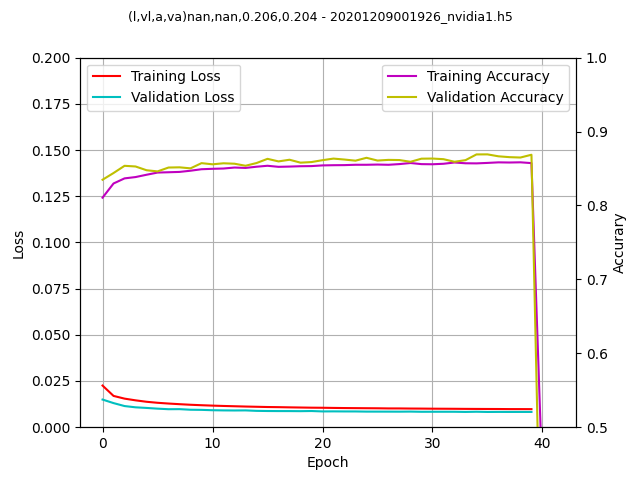
\includegraphics[width=\textwidth]{Figures/20201209001926_nvidia1_accuracy.png}
 \caption{nvidia1 trained on genRoad data for 100 epochs - stopped at 42 (best model saved)}
 \label{fig:20201209001926_nvidia1_accuracy} 
\end{figure}


%%% RUN 93 NVIDIA1 GEN ROAD 5 EPOCHS - STOPPED HERE - DOCUMENT
\begin{verbatim}
Epoch 4/5
3232/3232 [==============================] - 560s 173ms/step - loss: 0.0142 - acc: 0.8396 - val_loss: 0.0106 - val_acc: 0.8559
Epoch 5/5
3232/3232 [==============================] - 560s 173ms/step - loss: 0.0136 - acc: 0.8422 - val_loss: 0.0101 - val_acc: 0.8494
    
\end{verbatim}








%From Andrey

Hello Daniel.

The working version of the source code is submitted in an additional archive file. It should be ready for inspection and building.

The original fragments of the source code should be compiled int a single text document and submitted for the originality check as an appendix for the report.

You can make the old versions of the code available for audit from the cloud storage.

 

Keep safe.

Regards.

Andrey.


\end{appendices}

\end{document}  
